\chapter{Configurations avancées de ToM+}

\section{La page des paramètres Wi-Fi}
\label{sec:wifi_settings}

Depuis la deuxième version du firmware, votre ToM+ peut désormais se connecter à Internet grâce à un module Wi-Fi intégré. Cela vous permettra de consulter les données en temps réel de votre Twizy si vous le combinez avec le protocole MQTT, qui sera traité dans la Section~\ref{sec:MQTT}.\\

\begin{figure}[H]
    \centering
    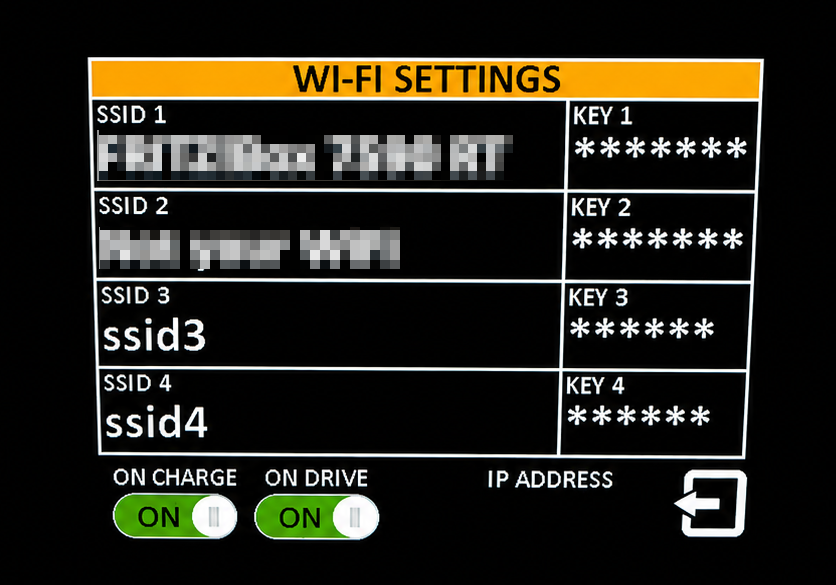
\includegraphics[width=0.8\textwidth]{figures/wifi_settings_3d.png}
    \caption{La page des paramètres Wi-Fi.}
\end{figure}

La page enregistrera jusqu'à quatre profils de connexion afin d'être connecté à Internet lorsque vous êtes à la maison, au travail ou dans un lieu public disposant d'un Wi-Fi gratuit.
\\De plus, ToM+ dispose d'une interface web dans laquelle vous pouvez surveiller les données en temps réel ou personnaliser vos paramètres beaucoup plus facilement. Voyons maintenant pourquoi vous devriez faire cela…

\subsection{Avantages du Wi-Fi ToM+}

Depuis la deuxième version du firmware, votre ToM+ peut désormais se connecter à Internet grâce à un module Wi-Fi intégré, ce qui vous permettra de débloquer beaucoup plus de fonctionnalités qu'auparavant.
Vous pouvez désormais accéder aux données de votre Twizy à distance sur votre smartphone !\\

Vous n'aurez plus besoin de vérifier manuellement l'état de charge de votre Twizy, car cette nouvelle fonctionnalité publiera les données de l'état de charge directement sur votre smartphone, de manière sécurisée et privée. Il suffira d'une simple configuration MQTT.\\

\begin{itemize}
    \item Fini la galère de devoir vérifier constamment l'état de charge de votre Twizy manuellement !
    \item De nombreuses possibilités d'intégrer votre Twizy dans un système IoT reposant sur MQTT
    \item Le Wi-Fi n'impacte presque pas la consommation électrique ni les performances de ToM
    \item Débloquez une nouvelle page web avec les données Twizy en temps réel et des paramètres ToM conviviaux
\end{itemize}

\subsection{Ajouter un profil de connexion Wi-Fi}
\label{sec:add_wifi_profile}

Dans cette nouvelle page de paramètres, vous disposez d'un petit tableau avec quatre lignes et deux colonnes.
La première colonne contient le \textbf{SSID} (c'est-à-dire le nom) du réseau auquel vous essayez de vous connecter. 
Pour être clair, c'est celui que vous voyez sur votre téléphone ou votre ordinateur portable. Il peut être alphanumérique et sensible à la casse (les majuscules comptent, assurez-vous donc de l'orthographier correctement !).
La deuxième colonne, sous l'en-tête \textbf{« KEY »}, est destinée au mot de passe Wi-Fi.\\

Lorsque vous appuyez sur une cellule du tableau, qu'il s'agisse du SSID ou de la clé, ToM+ ouvre une page de clavier sur laquelle vous pouvez saisir vos données. Appuyer sur OK confirmera la chaîne saisie et vous ramènera à la page des paramètres Wi-Fi. Nous aborderons la page du clavier dans la Section~\ref{sec:keyboard_page}.\\

Vous êtes désormais en mesure de configurer \textbf{quatre profils de connexion différents} avec quatre paires de SSID et de mots de passe. Si vous ne configurez aucun profil mais que les curseurs Wi-Fi sont activés, ToM+ effectuera tout de même une recherche Wi-Fi toutes les deux minutes pour essayer de trouver des connexions publiques sans protection par mot de passe, puis tentera de s'y connecter. Appuyez sur le bouton \textbf{flèche en bas à droite pour enregistrer}.\\

Le quatrième profil de connexion Wi-Fi est spécial, car le champ \textbf{« KEY 4 »} sert à la fois de champ de mot de passe standard pour le dernier SSID et à modifier le mot de passe par défaut du serveur web, comme cela sera abordé dans la Section~\ref{sec:web_change_password}.

De plus, vous pouvez saisir certains codes spéciaux dans ce champ pour effectuer des configurations secrètes. Ces codes sont sensibles à la casse et n'affecteront pas votre champ \textbf{« KEY 4 »} s'ils sont écrits correctement, car ToM+ les utilise uniquement comme des commandes. Vous pouvez saisir \textbf{GIVE\textunderscore ME\textunderscore DF!} (exactement comme écrit ici, avec les tirets bas et le point d'exclamation) pour \textit{afficher la numérotation et la description des erreurs DF} sur l'écran et sur l'interface webUI.\\

\textbf{RAPPEL !} Les commandes ne sont exécutées par ToM+ que si elles sont saisies depuis cette page de paramètres Wi-Fi, et non depuis l'interface webUI abordée plus tard. De plus, l'origine du numéro DF n'étant pas claire, l'activation de cette fonction est à votre discrétion et sous votre responsabilité.

\clearpage

\subsection{Vérifier la connexion Wi-Fi}
\label{sec:check_wifi_connection}

Pour vérifier si votre ToM+ est connecté à Internet via Wi-Fi, la procédure est très simple. Sur toutes les pages se trouve l'icône Wi-Fi (traitée dans la Section~\ref{sec:status_icon_bar}) qui indique son statut.

\iconbox{icons/Tray_WiFiOff.png}
{Wi-Fi désactivé}
{ToM+ n'est pas connecté et ne publiera aucune donnée.}

\iconbox{icons/Tray_WiFi.png}
{Wi-Fi activé}
{ToM+ est connecté et publiera des données si le protocole MQTT est connecté.}

\iconbox{icons/Tray_WiFi.png}
{Recherche Wi-Fi en cours}
{Si l'icône clignote, ToM+ recherche actuellement les réseaux Wi-Fi disponibles.}

Si vous souhaitez obtenir des informations plus spécifiques pour savoir si votre ToM+ est connecté à un réseau, vous pouvez consulter des champs supplémentaires dans la page des paramètres Wi-Fi, dans le coin inférieur droit, comme illustré dans l'image ci-dessous.

\begin{figure}[H]
    \centering
    
\includegraphics[width=0.7\textwidth]{figures/wifi_bottom_line.png}
    \caption{Informations de la grille inférieure Wi-Fi.}
    \label{fig:wifi_bottom_line}
\end{figure}

Comme nous pouvons le voir, lorsque le ToM+ est connecté à un réseau, une adresse IP s'affiche (ici c'est \textbf{10.24.126.204}). Il s'agit de l'adresse prise par ToM+ pour se connecter à Internet. Si ce champ contient une séquence de quatre nombres (de 0 à 255) séparés par des points, le Wi-Fi est connecté ; sinon, il sera vide.

Appuyez dessus pour afficher l'adresse MAC de ToM+ et appuyez à nouveau pour voir à quel SSID (nom de réseau) ToM+ est connecté. Nous verrons d'autres fonctionnalités intéressantes impliquant l'adresse IP de ToM+ plus tard dans la Section~\ref{sec:web_server_access}.

\subsection{Activer/Désactiver les fonctionnalités Wi-Fi}
\label{sec:enable_disable_wifi}

Dans le pied de page de la page des paramètres Wi-Fi, se trouvent deux boutons coulissants. Pour passer de l'état ON à OFF, il suffit de tapoter ou de faire glisser le bouton. Voyons ce que font ces deux curseurs.\\

Le premier d'entre eux permet de désactiver le \textbf{Wi-Fi pendant la charge}. Cela rendra votre ToM+ complètement hors ligne, et vous ne pourrez plus surveiller les données de votre Twizy à distance tant que vous ne l'aurez pas réactivé. Dans cet état, l'icône de statut Wi-Fi sera toujours grisée, comme montré dans la Section~\ref{sec:check_wifi_connection}.\\

Le deuxième bouton coulissant permet d'activer le \textbf{Wi-Fi pendant la conduite}. Cela permettra à votre ToM+ de rester connecté à Internet même lorsque vous conduisez votre Twizy. C'est utile si vous souhaitez publier des données en temps réel sur votre smartphone via MQTT. Cela permet également d'accéder à l'interface web tout en conduisant, et votre ToM+ recherchera aussi les réseaux Wi-Fi disponibles.\\

Comme déjà mentionné, pour \textit{enregistrer vos modifications}, vous devez appuyer sur le bouton fléché en bas à droite. Si vous ne le faites pas, vos modifications seront perdues lorsque vous quitterez la page.

\clearpage

\section{La page des paramètres MQTT}
\label{sec:MQTT}

Si vous avez déjà jeté un œil à la Section~\ref{sec:wifi_settings} sur le Wi-Fi, vous savez probablement déjà que le MQTT est nécessaire pour accéder à vos données à distance. Cette section vous montrera comment le configurer correctement et comment l'interface ToM+ gère ce protocole.

\begin{figure}[H]
    \centering
    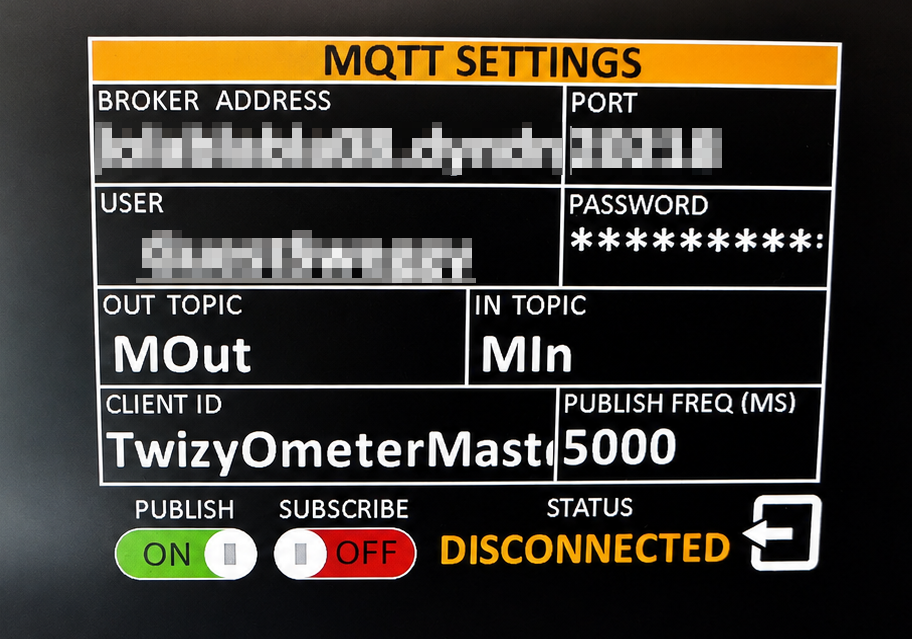
\includegraphics[width=0.8\textwidth]{figures/mqtt_settings_page.png}
    \caption{La page des paramètres MQTT.}
\end{figure}

Lorsque ToM+ est connecté à Internet via le Wi-Fi, le MQTT peut être activé pour vous permettre de consulter les données en temps réel de votre Twizy directement sur vos appareils. La page n'autorise qu'une seule configuration de serveur MQTT, afin de garantir la \textbf{sécurité et la confidentialité des données}. Vous pouvez configurer ces paramètres sur ToM+ ainsi que sur la page de son serveur web (Section~\ref{sec:web_network_settings}).
Présentons maintenant ce qu'est le MQTT et certains de ses principaux avantages…

\subsection{Brève explication du protocole MQTT}
\label{sec:brief_mqtt}

Le MQTT est l'un des protocoles les plus simples utilisés en informatique pour communiquer de petits volumes de données en utilisant une \textbf{architecture client/serveur}. Cette méthode nécessite un ou plusieurs clients qui collectent généralement des données, souhaitent les stocker de manière permanente et/ou effectuer des calculs.

Le processus nécessite donc un serveur qui traite les données de tous les clients exécutant des tâches. Ce serveur est appelé \textbf{broker MQTT} ou couramment broker, et il est essentiel dans ce type d'architecture. Mais comment les clients et le serveur communiquent-ils entre eux ?\\

Le processus de communication repose sur une structure de type publication/abonnement (publish/subscribe). Certains clients collectent et publient des données : ils sont appelés \textbf{éditeurs (publishers)}. Pendant ce temps, d'autres attendent que ces données soient envoyées : on les appelle les \textbf{abonnés (subscribers)}. Le serveur broker se situe au milieu et constitue le dispositif intermédiaire sur lequel toutes les données des éditeurs sont stockées et envoyées aux abonnés. Présentons maintenant les topics…\\

Un \textbf{topic} est une séquence de caractères alphanumériques généralement liée à un sujet spécifique. Il est utilisé pour stocker (comme un conteneur) toutes les données relatives à ce sujet. Les topics sont utiles pour conserver et organiser une grande quantité de données collectées auprès de différents éditeurs afin de ne pas confondre ces informations. Alors, comment ToM+ utilise-t-il le MQTT ?

\subsection{Communications ToM+ et MQTT}

Maintenant que nous savons ce qu'est le MQTT, voyons comment fonctionnent concrètement le système ToM+ et le MQTT.
ToM+ est considéré comme un éditeur (publisher), car il collecte et publie les données mises à jour de la Twizy. L'application mobile, quant à elle, sera l'abonné (subscriber) puisqu'elle attend de recevoir les données que la Twizy vient de publier. Mais qui est au milieu ? Le serveur broker.\\

À moins que vous ne disposiez d'un serveur broker auto-hébergé (comme c'est mon cas) ou que vous en connaissiez déjà un à utiliser, je vais vous expliquer comment configurer votre serveur broker externe gratuit dans la Section~\ref{sec:free_broker}.

Ainsi, combiner ToM+ avec le protocole MQTT peut s'avérer très puissant et, si vous aimez la domotique et les systèmes IoT, cela peut également débloquer des possibilités infinies. Par exemple, vous pouvez créer votre propre abonné qui réalisera des actions sur les données publiées par ToM+.\\

\subsection{Configuration d'un broker gratuit MQTT}
\label{sec:free_broker}

\textit{Avertissement} : Prenez votre temps lors de cette procédure, car pour les utilisateurs non expérimentés, cela peut prendre quelques minutes supplémentaires. Assurez-vous de bien \textbf{noter vos paramètres de configuration}.\\

Tout d'abord, choisissez votre fournisseur de broker MQTT. Je recommande personnellement Maqiatto, car il est gratuit, intuitif et facile à utiliser. Visitons donc la page de tutoriel de leur site officiel :
\url{https://www.maqiatto.com/examples}. Nous devrions maintenant voir une page semblable à celle présentée ici :

\begin{figure}[H]
    \centering
    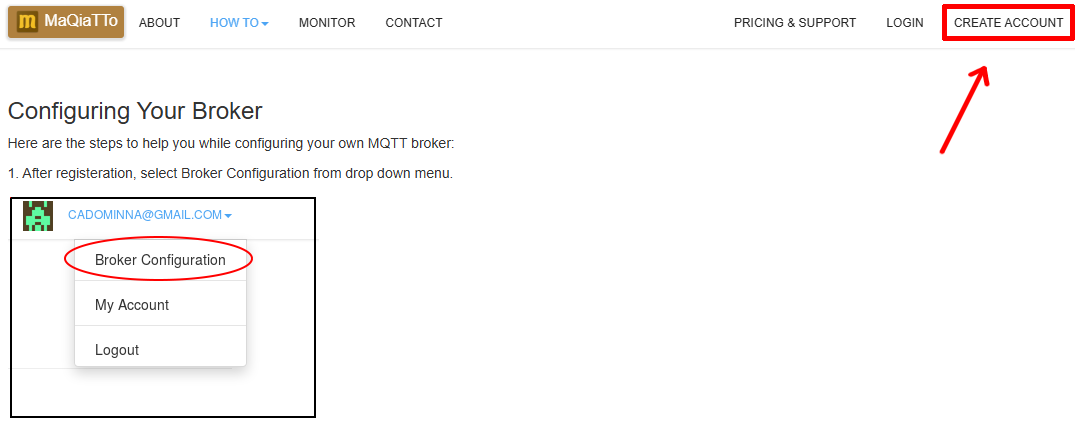
\includegraphics[width=1\textwidth]{figures/mqtt_step1.png}
    \caption{Étape 1 : Appuyez sur le bouton « CREATE ACCOUNT ».}
\end{figure}

Comme l'indique le guide officiel, vous devez disposer d'un compte afin de créer votre broker MQTT. Appuyons donc sur le bouton entouré en haut à droite \textbf{« Create Account »} pour en créer un.
Vous serez réorienté vers cette page (\url{https://www.maqiatto.com/signup}) où vous devrez remplir vos données personnelles.

\begin{figure}[H]
    \centering
    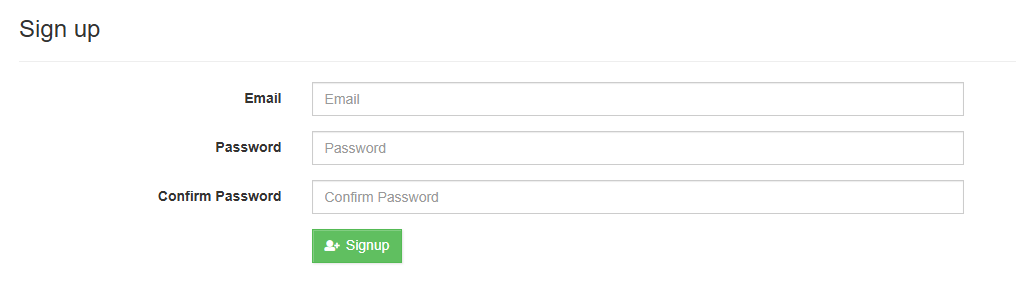
\includegraphics[width=1\textwidth]{figures/mqtt_step2.png}
    \caption{Étape 2 : Remplissez vos données personnelles.}
\end{figure}

Après avoir rempli tous les champs du formulaire, appuyez sur le bouton vert \textbf{« Signup »} et attendez d'obtenir cette page (\url{https://www.maqiatto.com/configure}) affichant un message de confirmation d'inscription, comme le montre l'image ci-dessous :

\begin{figure}[H]
    \centering
    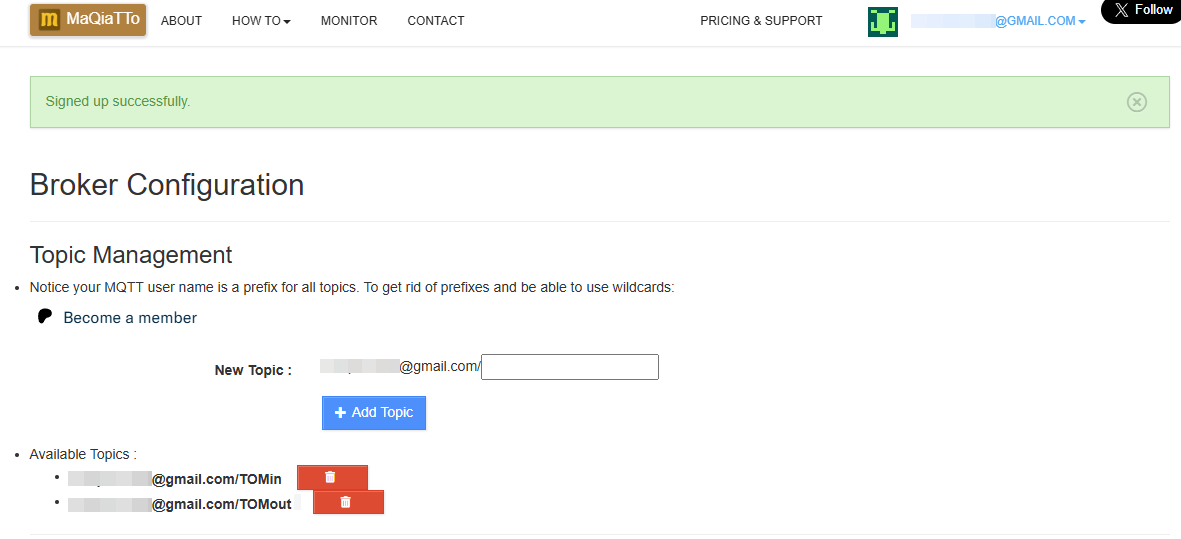
\includegraphics[width=1\textwidth]{figures/mqtt_step3.png}
    \caption{Étape 3 : Ajoutez les topics IN/OUT.}\label{sec:free_broker_add_topics}
\end{figure}

Depuis cette page, vous pouvez gérer vos topics disponibles (consultez la Section~\ref{sec:brief_mqtt}) et en créer de nouveaux. Créons donc nos topics IN et OUT pour envoyer et recevoir des données ToM. Comme nous pouvons le voir, il y a un préfixe fixe (votre adresse e-mail) car les utilisateurs gratuits ont cette limitation, mais ce n'est pas du tout un problème.\\

Dans la zone de texte vide après le symbole « / », nous devons saisir le nom que nous souhaitons donner à nos topics. Choisissez-le soigneusement et assurez-vous qu'il soit clair et facile à retenir pour vous. Par exemple, j'appellerai le topic d'entrée \textbf{TOMin} et le topic de sortie \textbf{TOMout}, mais vous pouvez choisir le nom que vous préférez.\\

Pour le premier topic, tapez \textbf{TOMin} et appuyez sur le bouton bleu \textbf{« + Add Topic »} comme je l'ai fait ci-dessus. Si l'opération réussit, un message vert s'affichera indiquant \textbf{« Topic was added for this user »} et un nouvel enregistrement apparaîtra dans la liste des \textit{« Available Topics »} qui était vide auparavant. Répétez maintenant le processus pour le topic \textbf{TOMout} et vérifiez à nouveau s'il a bien été créé. Avant cette procédure, la liste des \textit{« Available Topics »} était vide, mais nous pouvons désormais voir nos deux topics dans la liste et les supprimer si nécessaire.

\begin{figure}[H]
    \centering
    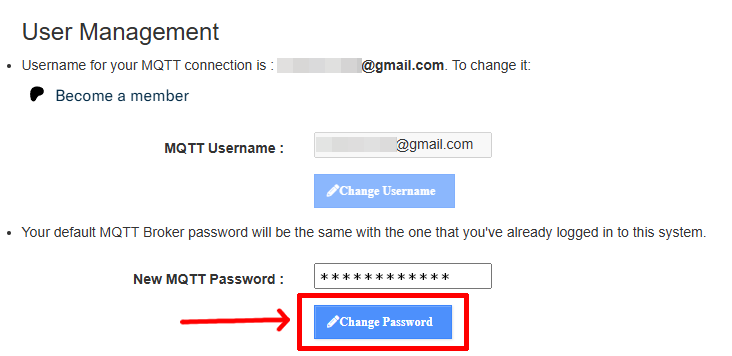
\includegraphics[width=0.8\textwidth]{figures/mqtt_step4.png}
    \caption{Étape 4 : Modifiez le mot de passe de votre broker.}
\end{figure}

\textit{Cette étape est suggérée mais facultative}. À ce stade, le mot de passe du broker est le même que celui de votre compte Maqiatto et n'est pas du tout sécurisé. Mais si vous ne souhaitez pas le modifier ou si cela ne vous importe pas, vous pouvez ignorer cette étape et passer à la suivante.\\

Prerenons donc le temps de sécuriser le broker afin de le protéger contre tout accès non autorisé. La seconde partie de cette page (\url{https://www.maqiatto.com/configure}) vous permet de modifier le mot de passe de votre broker.
Saisissez simplement le nouveau mot de passe dans le champ texte \textbf{« New MQTT Password »}, puis appuyez sur le bouton bleu \textbf{« Change Password »}.

Si tout se passe bien, un message vert apparaîtra indiquant \textbf{« Broker user password was updated »}. Le bouton de modification du nom d'utilisateur est grisé car vous ne pouvez pas modifier votre nom d'utilisateur à moins d'être un utilisateur premium.

\begin{figure}[H]
    \centering
    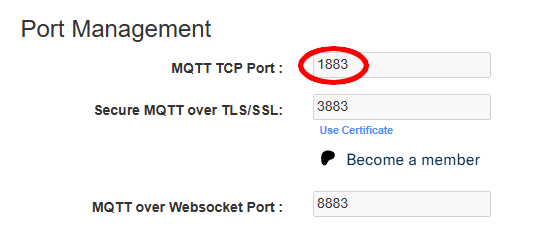
\includegraphics[width=0.7\textwidth]{figures/mqtt_step5.png}
    \caption{Étape 5 : Notez le numéro de port.}
\end{figure}

Dans la dernière section de la page de configuration (\url{https://www.maqiatto.com/configure}), se trouvent les paramètres de \textbf{« Port Management »}. Notez le port TCP MQTT qui est généralement défini sur \textbf{1883} (juste pour être sûr), car il s'agit du numéro de port standard bien connu sur Internet pour le protocole MQTT. Le broker MQTT est désormais prêt à être utilisé et nous pouvons passer à l'étape suivante, qui consiste à configurer ToM+ avec les paramètres du broker.

\clearpage

\subsection{Connecter ToM+ au broker MQTT}
\label{sec:mqtt_connection}

Maintenant que ce qu'est le MQTT est clair (Section~\ref{sec:brief_mqtt}) et que nous avons configuré notre broker personnel (Section~\ref{sec:free_broker}), voyons où sur l'écran nous pouvons connecter ToM+ avec notre broker fraîchement créé.

\begin{figure}[H]
    \centering
    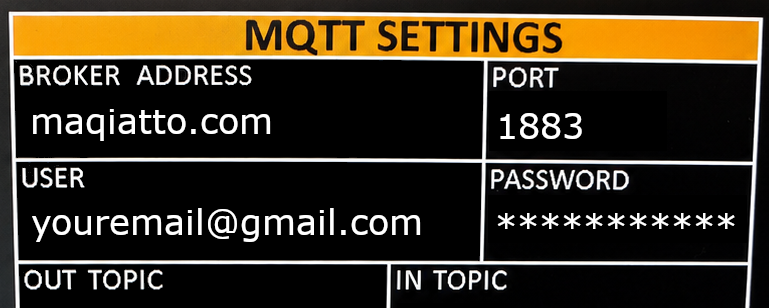
\includegraphics[width=0.8\textwidth]{figures/mqtt_connect1.png}
    \caption{Paramètres de connexion au broker MQTT.}
\end{figure}

Lorsque vous appuyez sur le champ correspondant du tableau, ToM+ ouvre une page de clavier sur laquelle vous pouvez saisir vos données, comme dans les paramètres Wi-Fi.
Pour insérer les symboles ou les chiffres, appuyez sur le bouton \textbf{« 1/3 »} du clavier pour changer de jeu de caractères.
En appuyant sur \textbf{OK}, vous confirmerez la chaîne saisie et cela vous ramènera à la page des paramètres MQTT. Pour en savoir plus sur la page du clavier, consultez la Section~\ref{sec:keyboard_page}.
Si la valeur est trop longue pour le champ, le texte défilera automatiquement.\\

La première chose à spécifier est l'adresse de votre \textbf{broker}. Dans l'exemple présenté, elle est définie sur \textit{« maqiatto.com »}. Il s'agit de l'adresse du serveur broker que nous venons de créer dans la Section~\ref{sec:free_broker}.

Il faut ensuite spécifier le \textbf{numéro de port} sur lequel le service MQTT s'exécute. À moins que vous ne l'ayez modifié manuellement, le port MQTT sera toujours le \textit{1883}.

Ensuite se trouve le champ \textbf{user}, qui correspond au nom d'utilisateur que ToM+ utilisera pour s'authentifier lors de la connexion au broker. La paire nom d'utilisateur et mot de passe étant unique pour vous, cela empêchera tout utilisateur indésirable d'accéder à votre broker privé. Dans votre cas, l'utilisateur est l'adresse e-mail de votre compte Maqiatto, écrite sous la forme \textit{votreemail@example.com}.

Ensuite, nous devons spécifier le \textbf{mot de passe du broker}, qui peut être différent de celui de votre compte Maqiatto si vous avez choisi de le modifier lorsqu'il a été suggéré dans la Section~\ref{sec:free_broker}.

\begin{figure}[H]
    \centering
    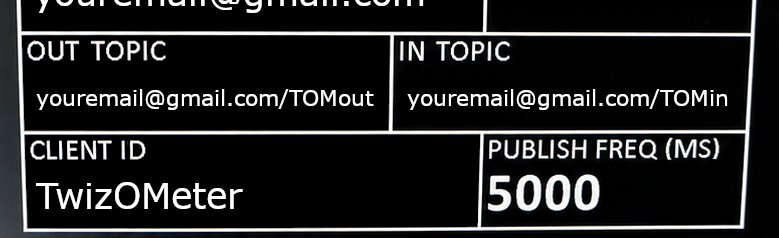
\includegraphics[width=0.8\textwidth]{figures/mqtt_connect2.png}
    \caption{Paramètres de publication MQTT de ToM+.}
\end{figure}

Configurons maintenant notre \textbf{topic OUT}, sur lequel ToM+ publiera les données de la Twizy. Dans la Section~\ref{sec:free_broker}, nous avons créé un topic de sortie appelé TOMout, mais le nom complet du topic doit également inclure \textbf{votre e-mail comme préfixe} suivi d'un symbole « / » et du nom du topic « TOMout ». Dans l'exemple, il est défini sur \textit{« votreemail@gmail.com/TOMout »}.

C'est maintenant au tour du \textbf{topic IN}, sur lequel ToM+ recevra les commandes MQTT.
Comme pour le topic OUT, nous avons créé un topic d'entrée appelé TOMin, mais le nom complet du topic doit également inclure \textbf{votre e-mail comme préfixe} suivi d'un symbole « / » et du nom du topic « TOMin ». Dans l'exemple, il est défini sur \textit{« votreemail@gmail.com/TOMin »}.

Lorsqu'un éditeur MQTT envoie un message au broker, sa connexion est authentifiée par nom d'utilisateur et mot de passe, mais il publie en utilisant un alias que \textit{vous pouvez choisir arbitrairement}. Il est important de ne pas inclure d'espaces dans le \textbf{Client ID} : seuls les caractères alphanumériques et les symboles sont autorisés. N'oubliez pas qu'il est conseillé de le rendre simple et clair comme dans l'exemple : \textit{« TwizOMeter »}.

Le dernier paramètre est la \textbf{fréquence de publication (publish frequency)}, qui représente l'intervalle de temps entre chaque publication de ToM+. Elle est exprimée en millisecondes \textit{(ms)} et peut être définie sur une valeur arbitraire supérieure à 1000ms (une seconde). La valeur par défaut est de \textit{5000 ms} (cinq secondes), ce qui constitue un bon compromis entre la fraîcheur des données et l'utilisation du réseau.\\

Pour \textbf{enregistrer vos modifications}, vous devez appuyer sur le bouton fléché en bas à droite. Si vous ne le faites pas, vos modifications seront perdues lorsque vous quitterez la page. ToM+ est désormais prêt à publier et recevoir des données via le protocole MQTT.\\

\subsection{Activer/Désactiver les fonctionnalités MQTT}
\label{sec:enable_disable_mqtt}

Si vous souhaitez désactiver temporairement ou définitivement la publication de données avec le protocole MQTT, appuyez ou faites glisser le curseur de gauche appelé \textbf{« PUBLISH »} dans l'image ci-dessous. Dès lors, ToM+ ne publiera plus les données de la Twizy via MQTT tant que vous ne l'aurez pas réactivé.

\begin{figure}[H]
    \centering
    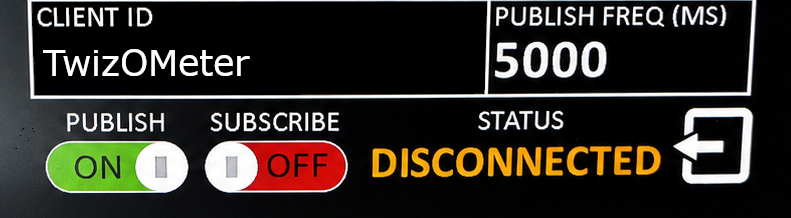
\includegraphics[width=0.8\textwidth]{figures/mqtt_connect3.png}
    \caption{Curseurs inférieurs MQTT.}
\end{figure}

Le bouton coulissant de droite sous \textbf{« SUBSCRIBE »} permet à ToM+ de recevoir des commandes provenant de périphériques externes publiées sur le topic IN spécifié. Cela est utile si vous souhaitez contrôler via MQTT un appareil connecté au port d'extension de ToM+ (par exemple, une prise connectée pour démarrer/arrêter la charge à distance). Vous pouvez choisir d'activer ou de désactiver cette fonctionnalité à tout moment en appuyant ou en faisant glisser le bouton.\\

\subsection{Vérifier la connexion MQTT de ToM+}

Près des deux boutons coulissants se trouve une petite étiquette \textbf{« STATUS »} qui indique si la connexion MQTT fonctionne ou non. Lorsque ToM+ est connecté au broker MQTT spécifié, le texte \textit{« CONNECTED »} s'affiche. En cas de problème de connexion au broker ou si le Wi-Fi est désactivé, comme nous l'avons vu dans la Section~\ref{sec:enable_disable_wifi}, le protocole MQTT ne fonctionnera pas correctement et un message \textit{« DISCONNECTED »} apparaîtra, comme sur l'image ci-dessous.

\begin{figure}[H]
    \centering
    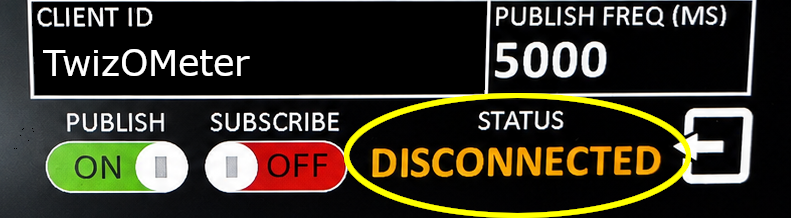
\includegraphics[width=0.8\textwidth]{figures/mqtt_status.png}
    \caption{Champ de statut MQTT.}
\end{figure}

Par ailleurs, vous pouvez également vérifier le statut de la connexion MQTT en regardant la barre d'icônes de statut (Section~\ref{sec:status_icon_bar}) où l'icône MQTT sera violette si la connexion est établie, sinon elle sera grisée.

Pour \textbf{enregistrer vos modifications}, vous devez appuyer sur le bouton fléché en bas à droite. Si vous ne le faites pas, vos modifications seront perdues lorsque vous quitterez la page.\\


\section{La page Clavier}
\label{sec:keyboard_page}

Lorsque vous appuyez sur une cellule de tableau dans la page des paramètres Wi-Fi ou MQTT, ToM+ ouvre une page de clavier sur laquelle vous pouvez saisir vos données. La page de clavier est très intuitive et facile à utiliser. Vous pouvez basculer entre trois jeux de caractères différents en appuyant sur le bouton \textbf{« 1/3 »} dans le coin inférieur gauche du clavier.

\begin{figure}[ht]
    \centering

    \begin{subfigure}[t]{0.48\textwidth}
        \centering
        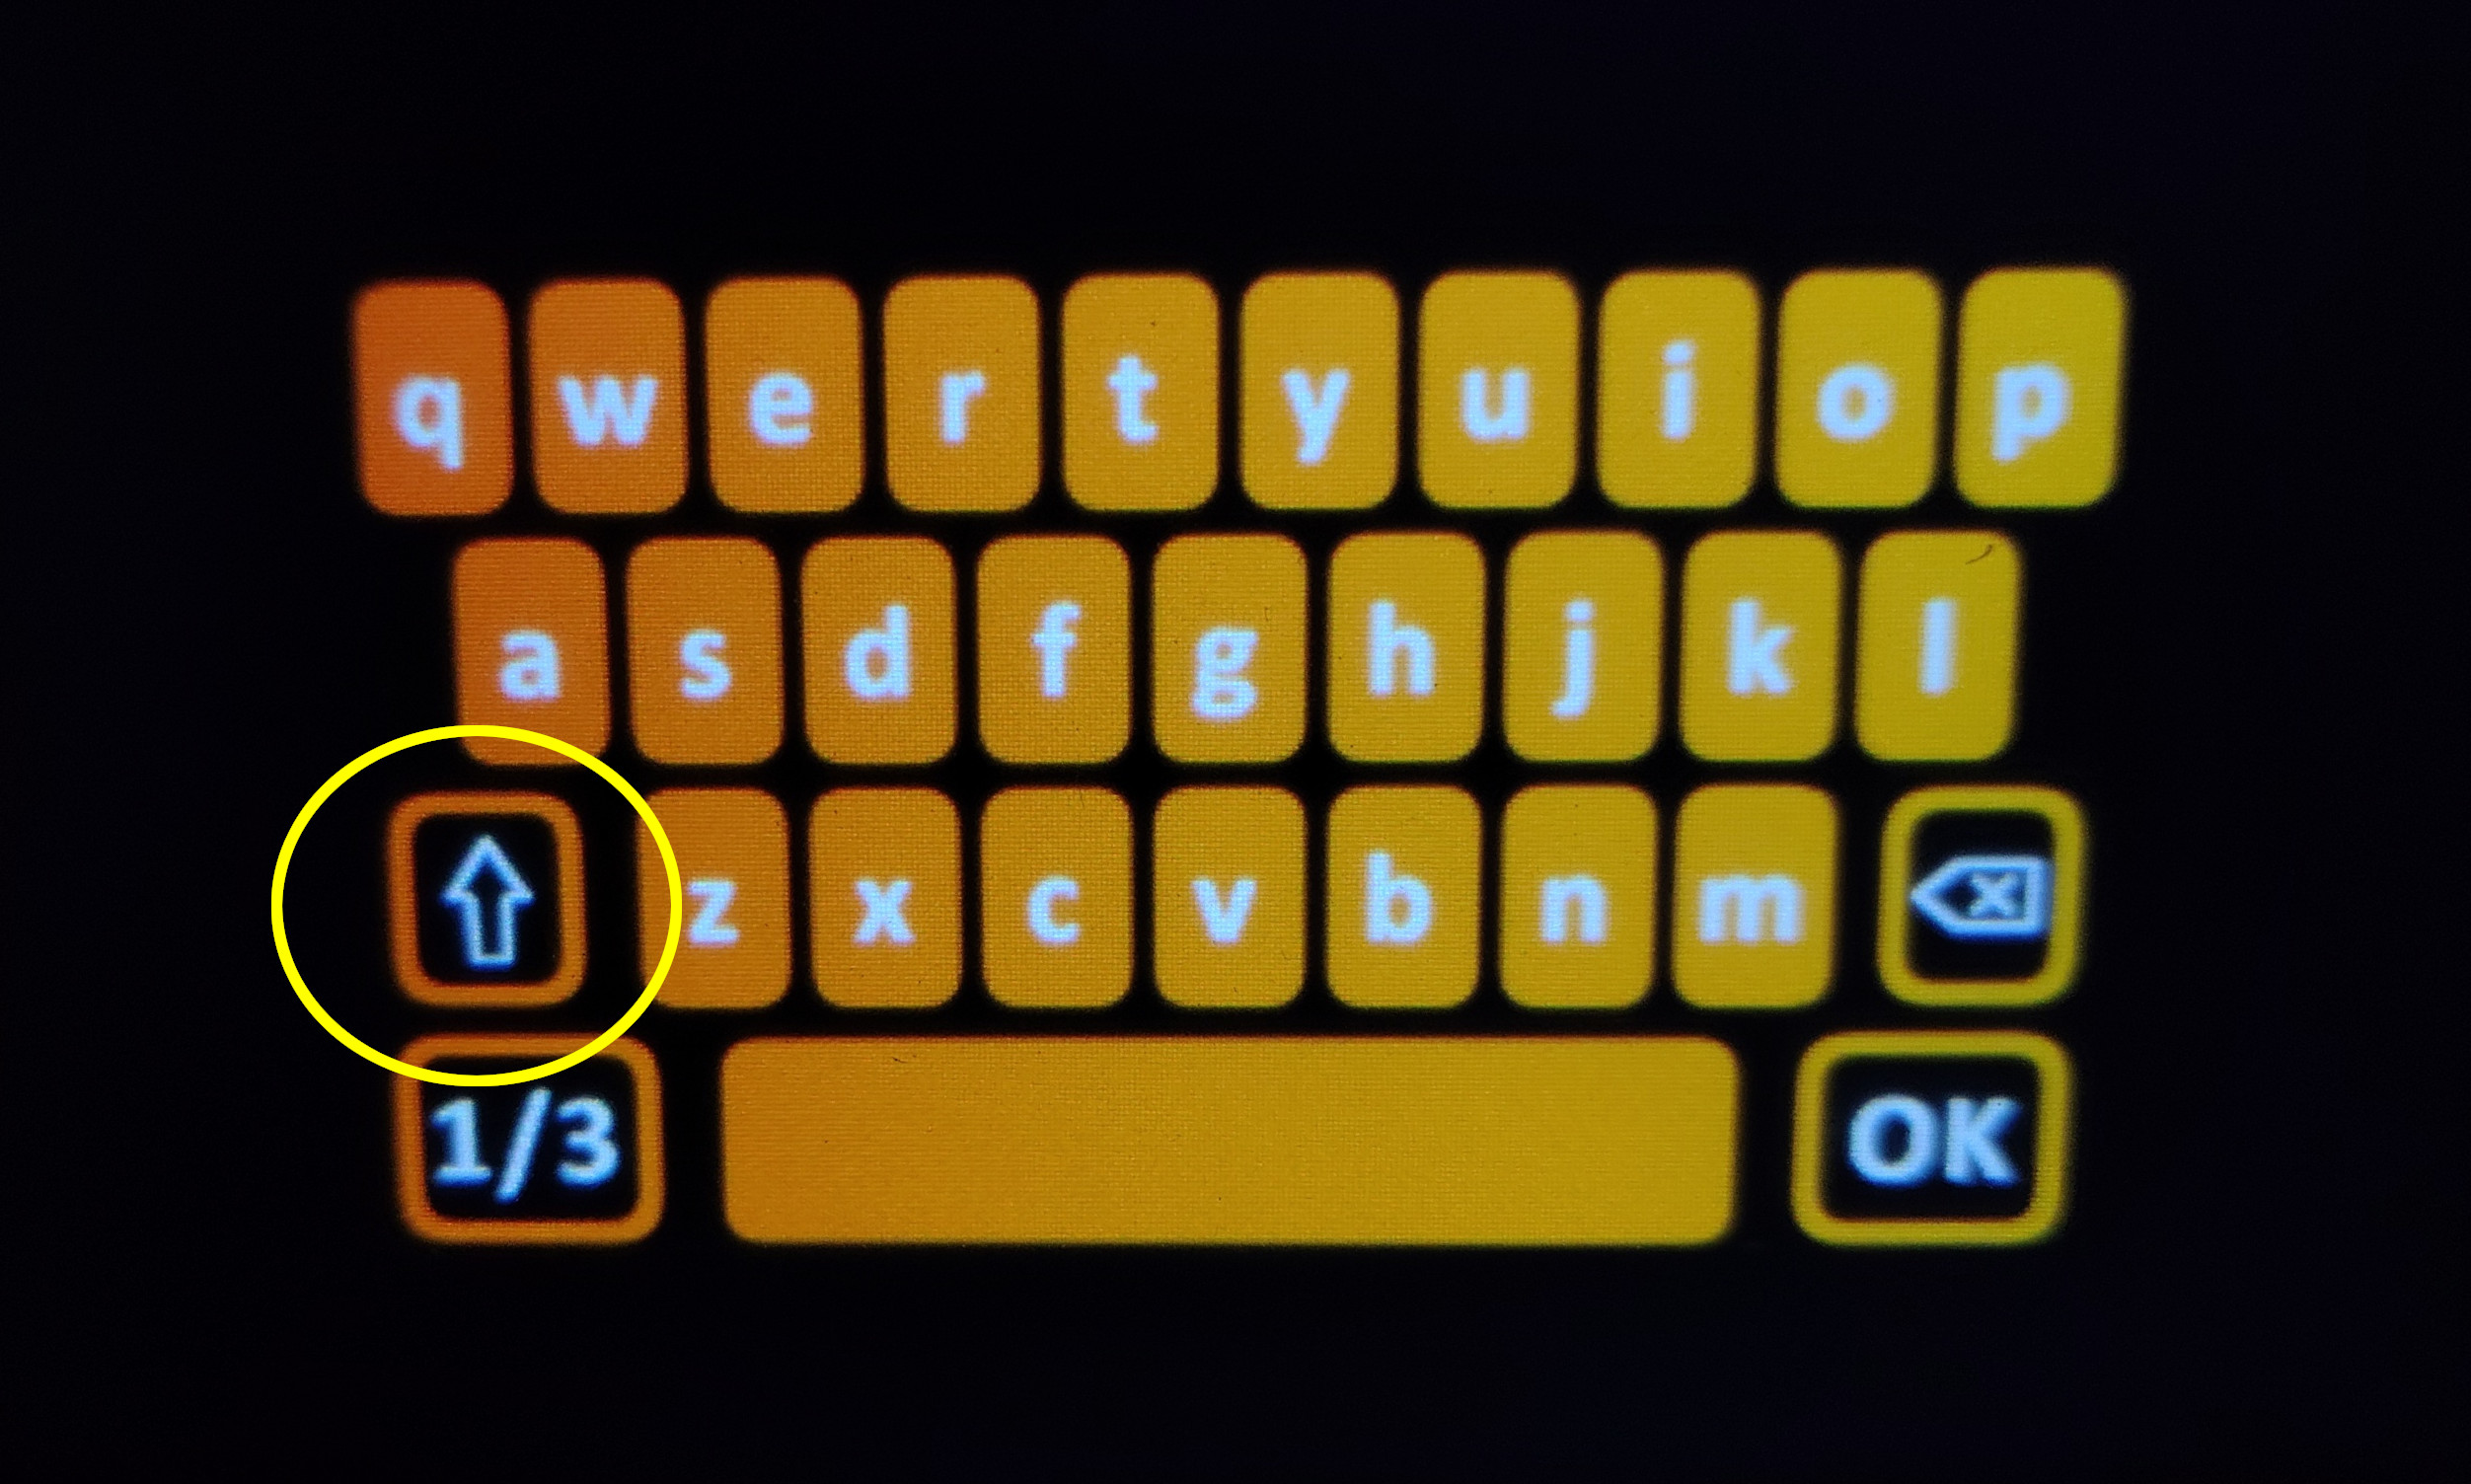
\includegraphics[width=\linewidth]{figures/keyboard_page1.jpg}
        \caption{Premier jeu de caractères : Lettres.}
    \end{subfigure}
    \hfill
    \begin{subfigure}[t]{0.48\textwidth}
        \centering
        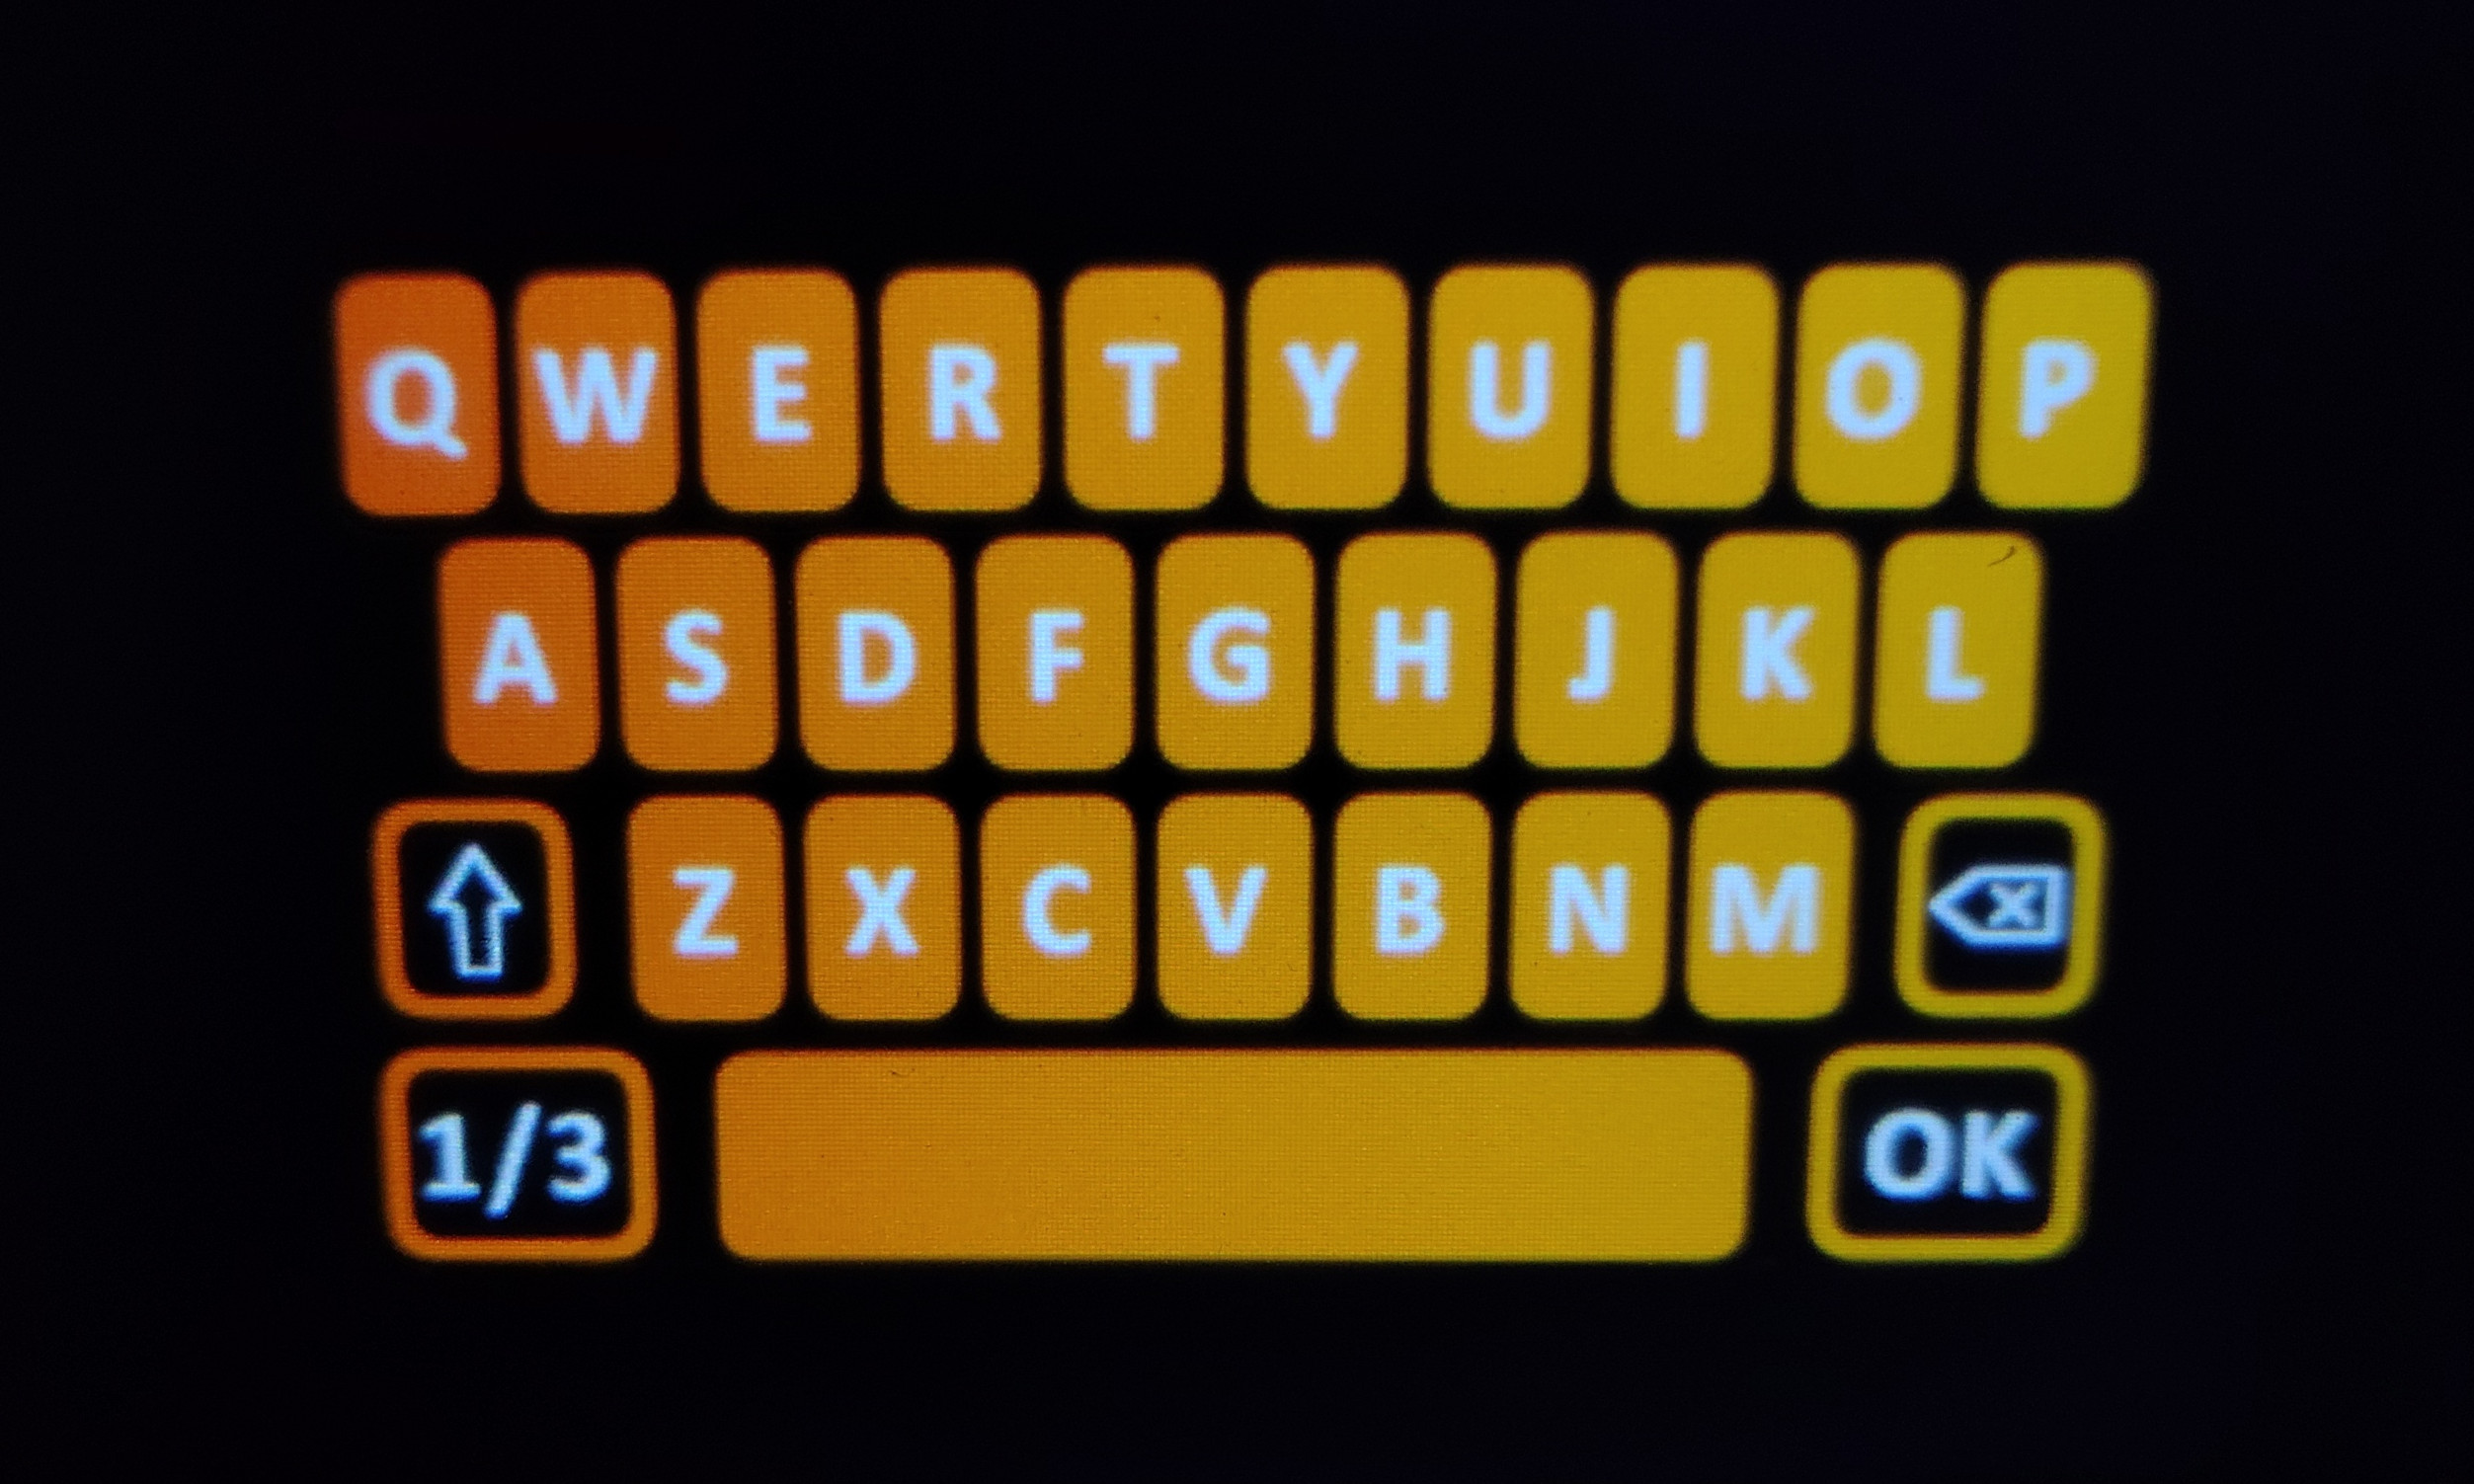
\includegraphics[width=\linewidth]{figures/keyboard_page1_caps.jpg}
        \caption{Premier jeu de caractères : Majuscules.}
    \end{subfigure}
\end{figure}

Dans le \textbf{premier jeu de caractères}, vous pouvez saisir des lettres en minuscules ou en majuscules en appuyant sur le bouton majuscule entouré en jaune dans la première image.
Lorsque vous saisissez quelque chose, cela apparaît dans le champ texte en haut du clavier. 
Si vous souhaitez supprimer un caractère, appuyez simplement sur la touche retour arrière.

\clearpage

\begin{figure}[ht]
    \centering

    \begin{subfigure}[t]{0.48\textwidth}
        \centering
        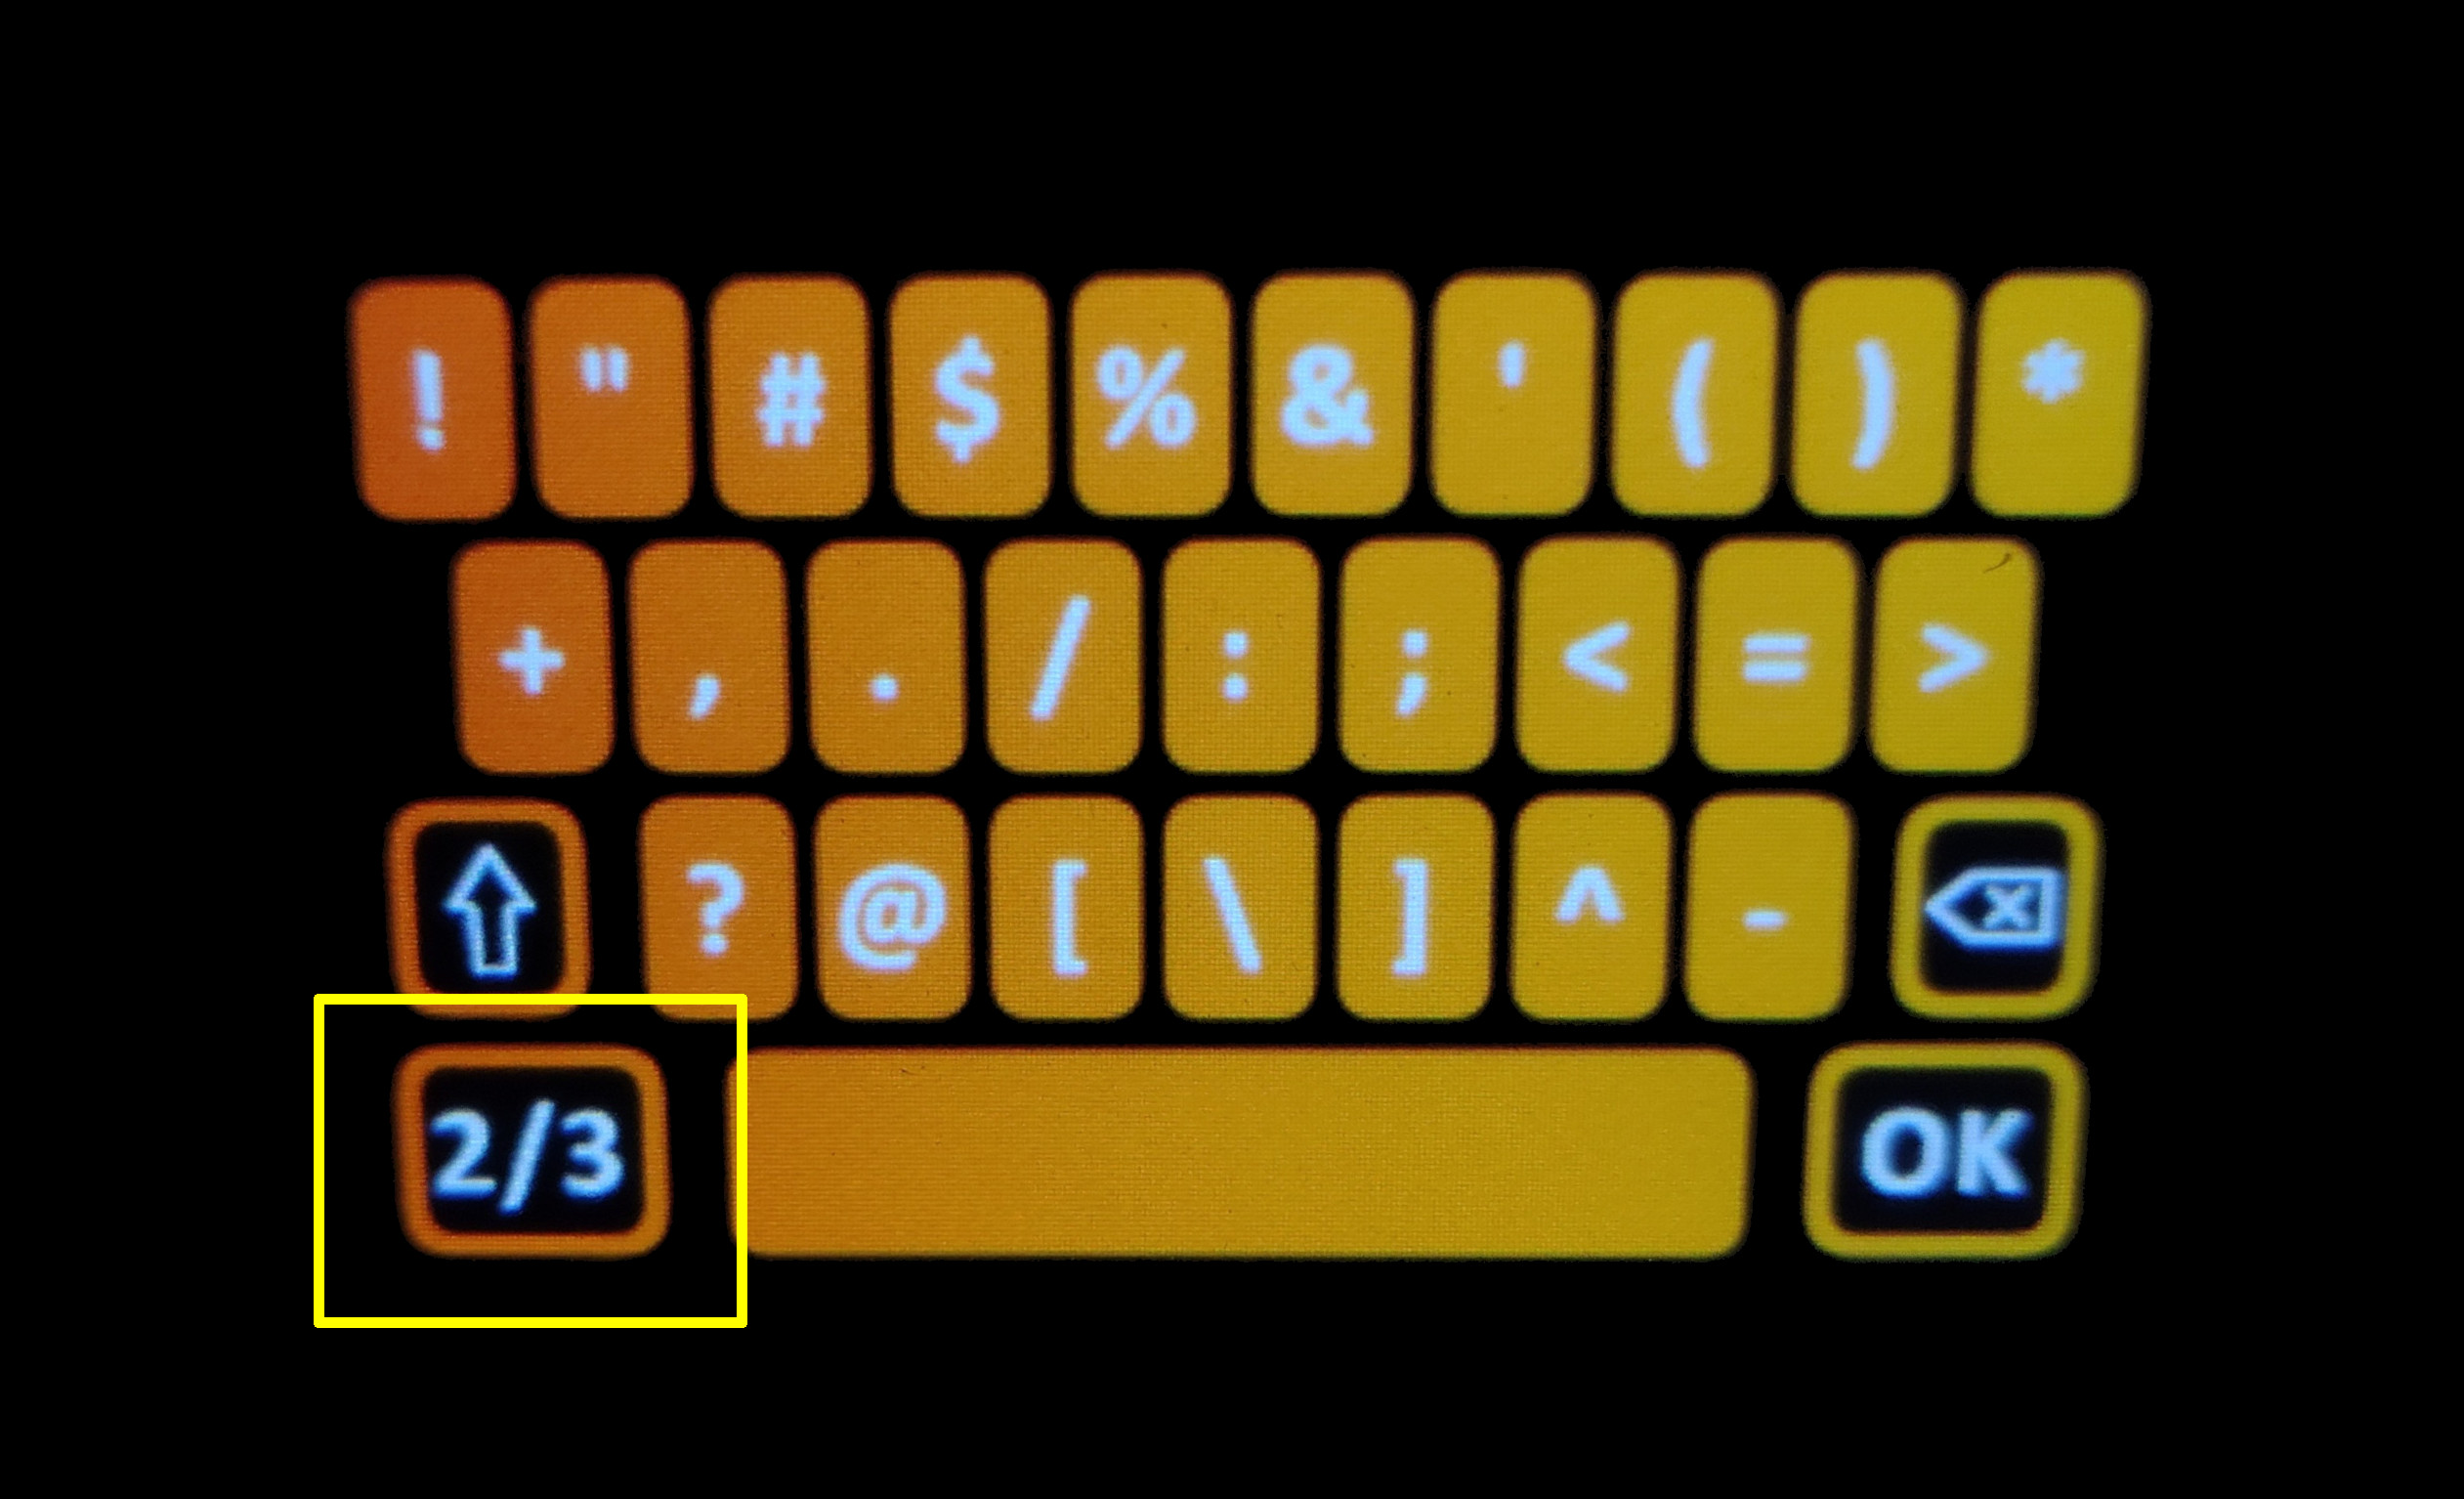
\includegraphics[width=\linewidth]{figures/keyboard_page2.jpg}
        \caption{Deuxième jeu de caractères : Symboles.}
    \end{subfigure}
    \hfill
    \begin{subfigure}[t]{0.48\textwidth}
        \centering
        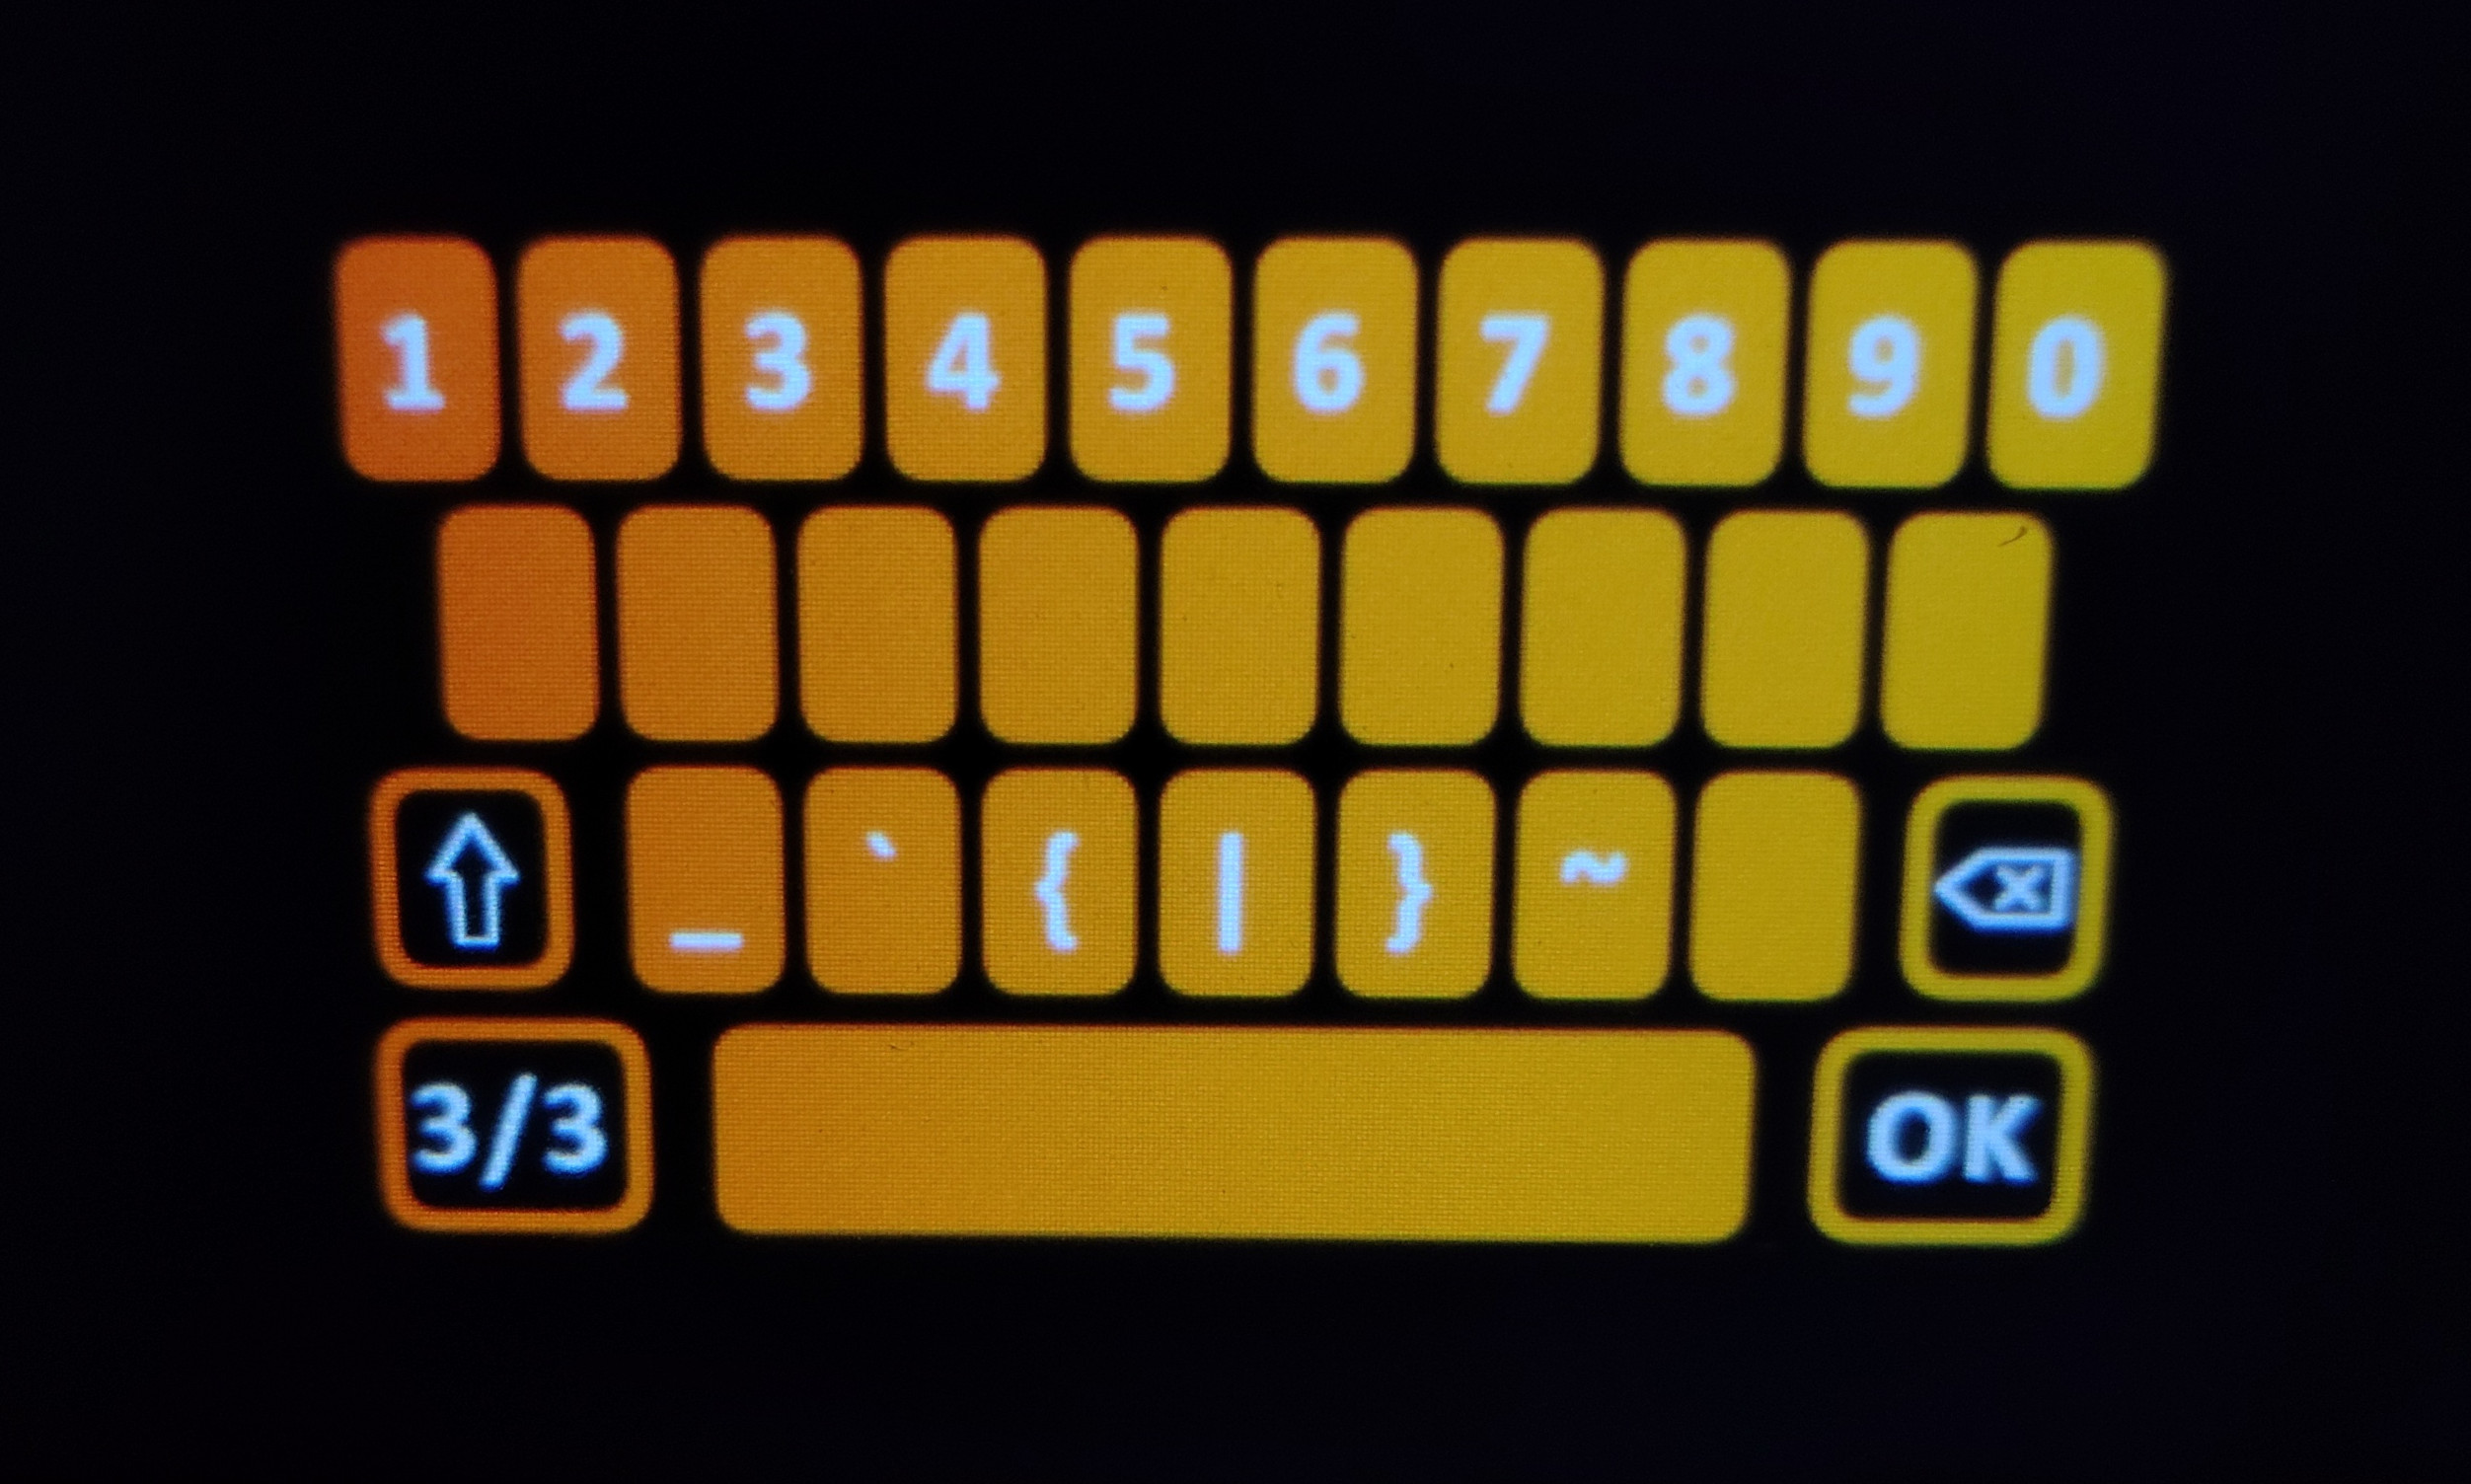
\includegraphics[width=\linewidth]{figures/keyboard_page3.jpg}
        \caption{Troisième jeu de caractères : Chiffres et plus.}
    \end{subfigure}
\end{figure}

Le \textbf{deuxième jeu de caractères} est destiné aux symboles et le \textbf{troisième} aux chiffres et autres caractères spéciaux.
Pour passer au troisième jeu de caractères, appuyez simplement sur le bouton \textbf{« 2/3 »} dans le coin inférieur gauche du clavier.
Une fois sur le troisième jeu de caractères, vous pouvez revenir au premier en appuyant sur le bouton \textbf{« 3/3 »}.
Sur ces deux pages, la touche majuscule ne fera rien car elle n'est pas nécessaire.\\

Lorsque vous avez terminé la saisie, appuyez sur le bouton \textbf{OK} pour confirmer votre saisie et revenir à la page de paramètres MQTT ou Wi-Fi précédente, où le champ modifié sera mis à jour.

\subsection{Le clavier numérique uniquement}

Dans certains champs, tels que la fréquence de publication MQTT, seuls les chiffres sont autorisés.
Dans ce cas, ToM+ ouvrira une page de clavier numérique uniquement, comme montré dans l'image ci-dessous.

\begin{figure}[H]
    \centering
    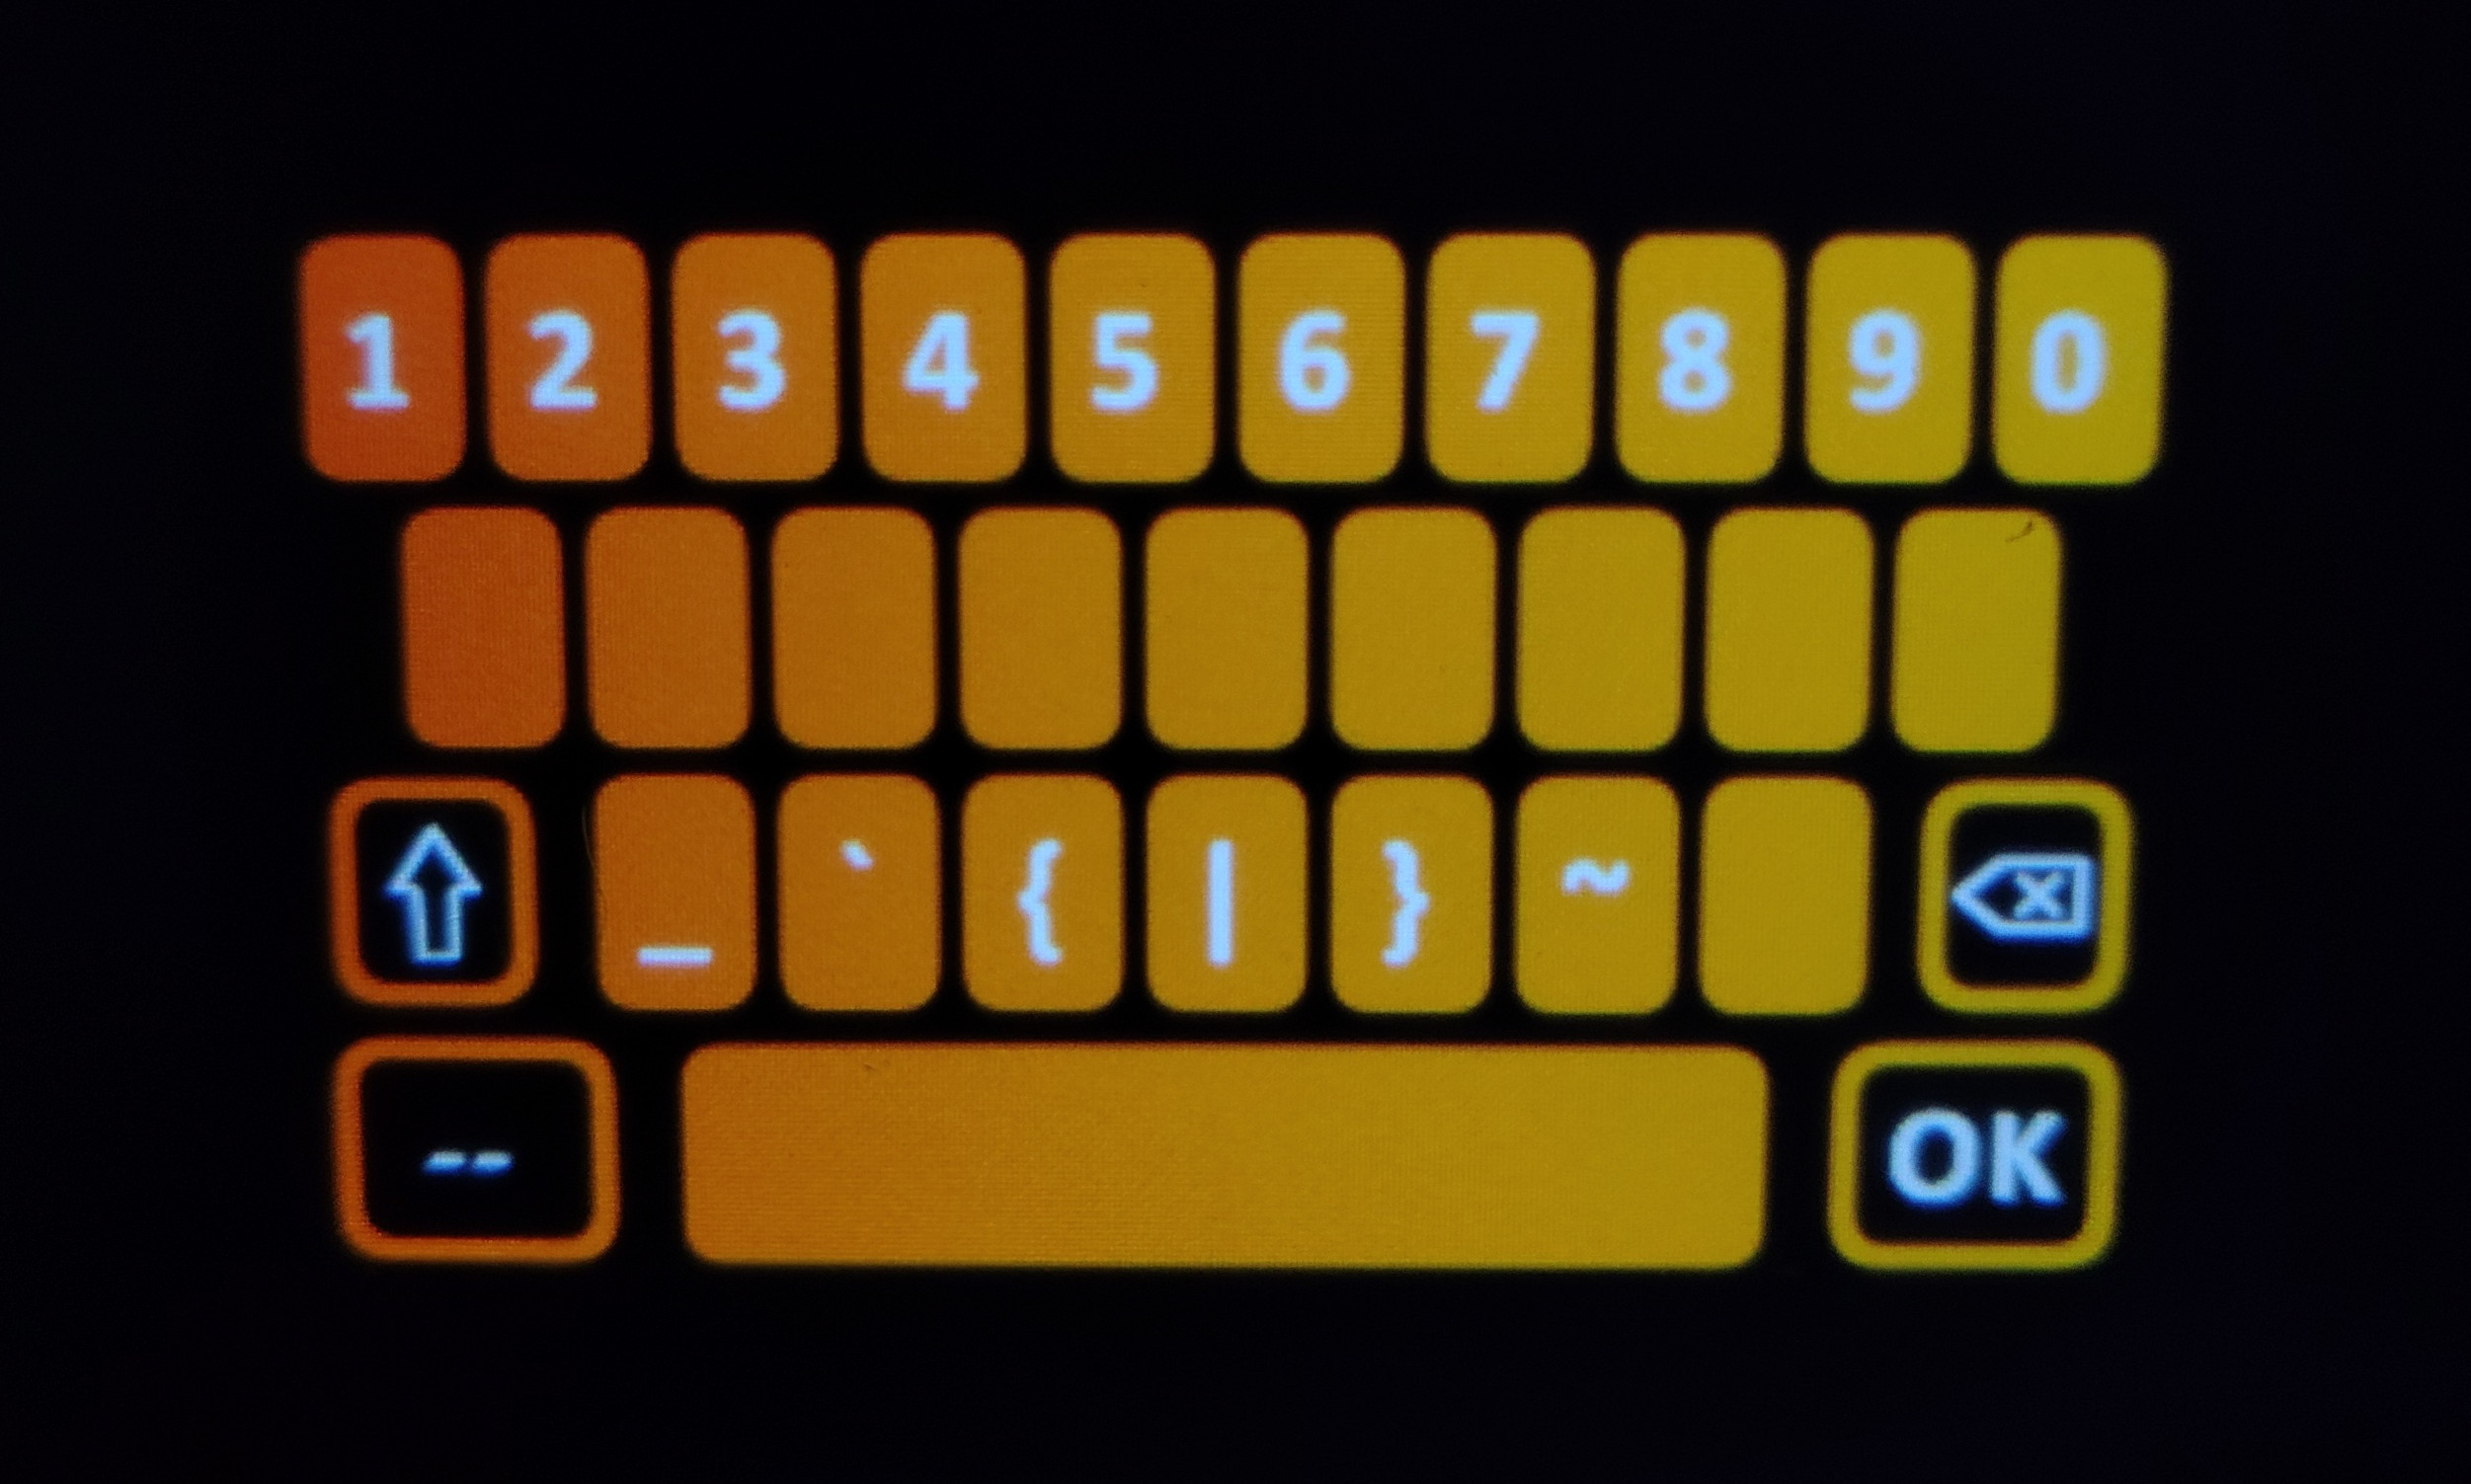
\includegraphics[width=0.8\textwidth]{figures/keyboard_num_only.jpg}
    \caption{Clavier numérique uniquement.}
\end{figure}

Comme vous pouvez le constater, la disposition est la même que celle du troisième jeu de caractères du clavier complet, mais elle est limitée aux chiffres et à quelques caractères spéciaux.
Vous pouvez également remarquer que le bouton de changement de jeu de caractères est indisponible, car il n'est pas nécessaire dans ce cas.
La touche retour arrière reste disponible pour supprimer des caractères, et le bouton \textbf{OK} confirme votre saisie puis retourne à la page précédente.



\section{Le serveur web}
\label{sec:web_server}

Le serveur web est une nouvelle fonctionnalité introduite avec la deuxième version du firmware. 
Il vous permet d'accéder aux paramètres et aux données de votre ToM+ à distance depuis n'importe quel appareil doté d'un navigateur web, comme votre smartphone, votre tablette ou votre PC. C'est particulièrement utile pour gérer les configurations standard et \textbf{avancées} qui ne sont pas disponibles sur l'écran du ToM+.

De plus, vous pouvez également utiliser le serveur web pour configurer le \textbf{Wi-Fi et le MQTT} bien plus facilement qu'en utilisant uniquement l'écran du ToM+ avec la page clavier (Section~\ref{sec:keyboard_page}).\\

\begin{figure}[H]
    \centering
    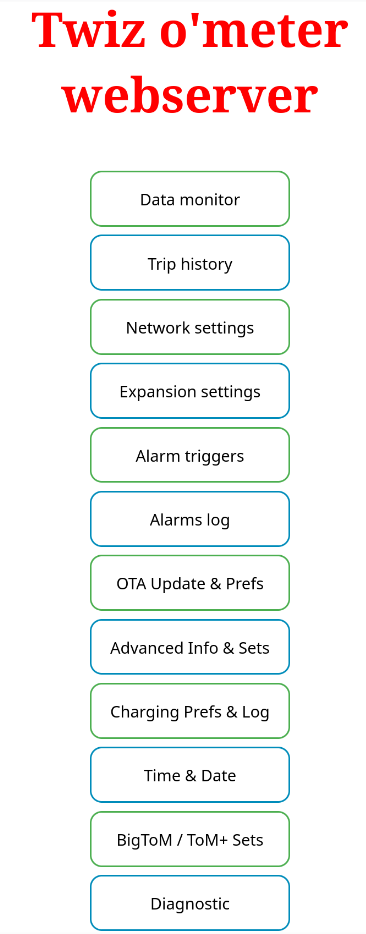
\includegraphics[width=0.46\textwidth]{figures/landing_page.png}
    \caption{Page d'accueil du serveur web.}
\end{figure}


\subsection{La page d'accueil}

Sur la page d'accueil illustrée ci-dessus, vous verrez douze boutons qui vous donnent accès aux différentes pages du serveur web.
Je vais donner ici un rapide aperçu des fonctions disponibles sur chaque page, puis elles seront toutes approfondies dans les paragraphes suivants. Dans cette section, les icônes ne servent qu'à titre d'aide visuelle :\\

\iconbox{icons/BatteryInfo2.png}
{Moniteur de données}{Vous pouvez surveiller ici les données de votre Twizy en temps réel, organisées sous forme de tableaux tout comme sur les pages d'affichage du ToM+ (Section~\ref{sec:web_data_monitor}).}

\iconbox{icons/Street0Ok_v2.png}
{Historique des trajets}{Vous pouvez consulter ici les données de chaque trajet enregistré (1 à 5) ainsi que les vingt derniers trajets, de la même façon que sur l'écran du ToM+ (Section~\ref{sec:web_trip_history}).}

\iconbox{icons/Tray_WiFiOff.png}
{Paramètres réseau}{Vous pouvez configurer ici vos profils de connexion Wi-Fi et les paramètres du broker MQTT, comme sur l'écran du ToM+ (Section~\ref{sec:web_network_settings}).}

\iconbox{icons/Pin1.png}
{Paramètres d'extension}{Vous pouvez configurer ici les broches du connecteur d'extension et choisir le comportement du bouton du commodo d'essuie-glace droit (Section~\ref{sec:web_expansion_settings}).}

\iconbox{icons/Alarm.PNG}
{Déclencheurs d'alarme}{Vous pouvez afficher ou configurer ici des alarmes basées sur les données de ToM+ et choisir l'action à exécuter lorsqu'une alarme se déclenche (Section~\ref{sec:web_alarm_triggers}).}

\iconbox{icons/Alarm.PNG}
{Journal des alarmes}{Vous pouvez consulter et effacer ici l'historique des 21 derniers déclenchements d'alarmes et leurs détails, tels que la date et l'heure (Section~\ref{sec:web_alarms_log}).}

\iconbox{icons/Swap.png}
{Mise à jour OTA \& Préf.}{Vous pouvez mettre à jour ici le firmware du ToM+ via la méthode OTA et sauvegarder/restaurer vos préférences ToM+ (Section~\ref{sec:web_ota_update}).}

\iconbox{icons/Swap.png}
{Infos avancées \& Régalges}{Vous pouvez consulter ici des informations avancées sur la batterie de votre Twizy et configurer divers paramètres (Section~\ref{sec:web_advanced_info}).}

\iconbox{icons/CEta.png}
{Préf. de charge \& Journal}{Vous pouvez configurer ici les préférences de charge, interrompre la charge à la volée, et consulter ou effacer les 15 derniers journaux de charge (Section~\ref{sec:web_charging_prefs}).}

\iconbox{icons/Timer.PNG}
{Heure \& Date}{Vous pouvez régler ici l'heure et la date de votre ToM+ et choisir le fuseau horaire à l'aide de chaînes POSIX TZ ou vous synchroniser avec le Wi-Fi (Section~\ref{sec:web_time_date}).}

\iconbox{icons/Kmh.png}
{Réglages BigToM / ToM+}{Vous pouvez configurer ici certains paramètres du tableau de bord, comme l'échelle de la barre de puissance ou définir une limite de vitesse (Section~\ref{sec:web_btom_tom_sets}).}

\iconbox{icons/Error.png}
{Diagnostic}{Vous pouvez consulter ici les numéros DTC/DF ainsi que les descriptions des erreurs de votre Twizy et effacer les journaux si nécessaire (Section~\ref{sec:web_diagnostic}).}


\subsection{Accéder au serveur web}
\label{sec:web_server_access}

ToM+ vous permet de vous connecter à la page de son serveur web de deux manières, toutes deux utiles dans différentes situations. Avant de commencer, gardez à l'esprit qu'une \textbf{adresse IP} est fondamentalement le nom numérique de votre appareil sur un réseau (par ex. \textit{192.168.1.100}).

\textbf{\textit{Pour les deux méthodes, vous devez connecter le ToM+ à un réseau.}}
Assurez-vous donc de vérifier si votre ToM+ dispose d'un profil Wi-Fi configuré comme expliqué dans la Section~\ref{sec:add_wifi_profile} ou s'il est connecté à un réseau Wi-Fi sans mot de passe.
Pour vérifier si votre ToM+ est connecté, veuillez vous référer à la Section~\ref{sec:check_wifi_connection}.\\

\textbf{La première méthode, la plus simple,} consiste à utiliser le point d'accès (hotspot) de votre téléphone sans mot de passe, afin que ToM+ se connecte sans avoir à configurer de profil Wi-Fi. Ensuite, toujours avec votre téléphone, ouvrez Chrome ou Safari (ou n'importe quel navigateur web) et saisissez l'adresse IP de ToM+ (telle qu'illustrée sur la Figure~\ref{fig:wifi_bottom_line}).\\

\textbf{La seconde méthode} ne fonctionne que si vous êtes assez proche de la Twizy, à portée du Wi-Fi.
Vous pouvez utiliser votre téléphone ou votre ordinateur portable pour effectuer une recherche Wi-Fi, puis chercher le réseau \textit{« ToM+ AP »}, \textit{« Twiz o'Meter AP »} ou \textit{« BigToM AP »}, selon votre modèle. 
Ensuite, connectez-vous à ce réseau avec le \textbf{bon mot de passe}. Il est initialement défini sur le mot « pass » suivi du numéro de série de votre appareil (par ex. \textit{pass129777}).
Le numéro de série se trouve sur la page des paramètres, comme expliqué dans la Figure~\ref{fig:settings_page}. 
Vous pourrez ensuite le modifier si vous le souhaitez, mais il n'existe pas de système de récupération de mot de passe (voir Section~\ref{sec:web_change_password}).
Une fois connecté au point d'accès de ToM+, saisissez son adresse IP statique sur n'importe quel navigateur, c'est-à-dire \textbf{192.188.1.188}.


\subsection{Changer le mot de passe du serveur web}
\label{sec:web_change_password}

Pour modifier le mot de passe du serveur web, allez sur la page des paramètres Wi-Fi de l'écran (Section~\ref{sec:wifi_settings}) et appuyez sur le champ \textbf{« KEY 4 »}. Cela ouvrira la page du clavier (Section~\ref{sec:keyboard_page}) où vous pourrez saisir votre nouveau mot de passe.
Ce mot de passe sera ainsi utilisé à la fois comme mot de passe du point d'accès et pour le quatrième profil de connexion Wi-Fi.


\subsection{Page du moniteur de données}
\label{sec:web_data_monitor}

Comme indiqué dans l'introduction, cette page répertorie toutes les données ToM+ disponibles, organisées en sept tableaux différents dont chacun ne contient que les données spécifiées dans son en-tête. La répartition des données est la même que celle utilisée dans la Section~\ref{sec:icon_list} et ne peut pas être modifiée.

Ces valeurs sont \textbf{mises à jour toutes les 10 secondes} et sont associées à leur unité de mesure. Ne vous inquiétez pas pour votre confidentialité car vos données voyagent encapsulées dans une structure de paquet particulière, difficile à intercepter ou à pirater. De plus, le serveur web n'utilise aucun service externe ni le protocole MQTT pour le contrôle, de sorte que vos données restent privées et sécurisées. La page est entièrement générée directement par le boîtier noir et ne subit aucun traitement ultérieur.

\begin{figure}[H]
    \centering
    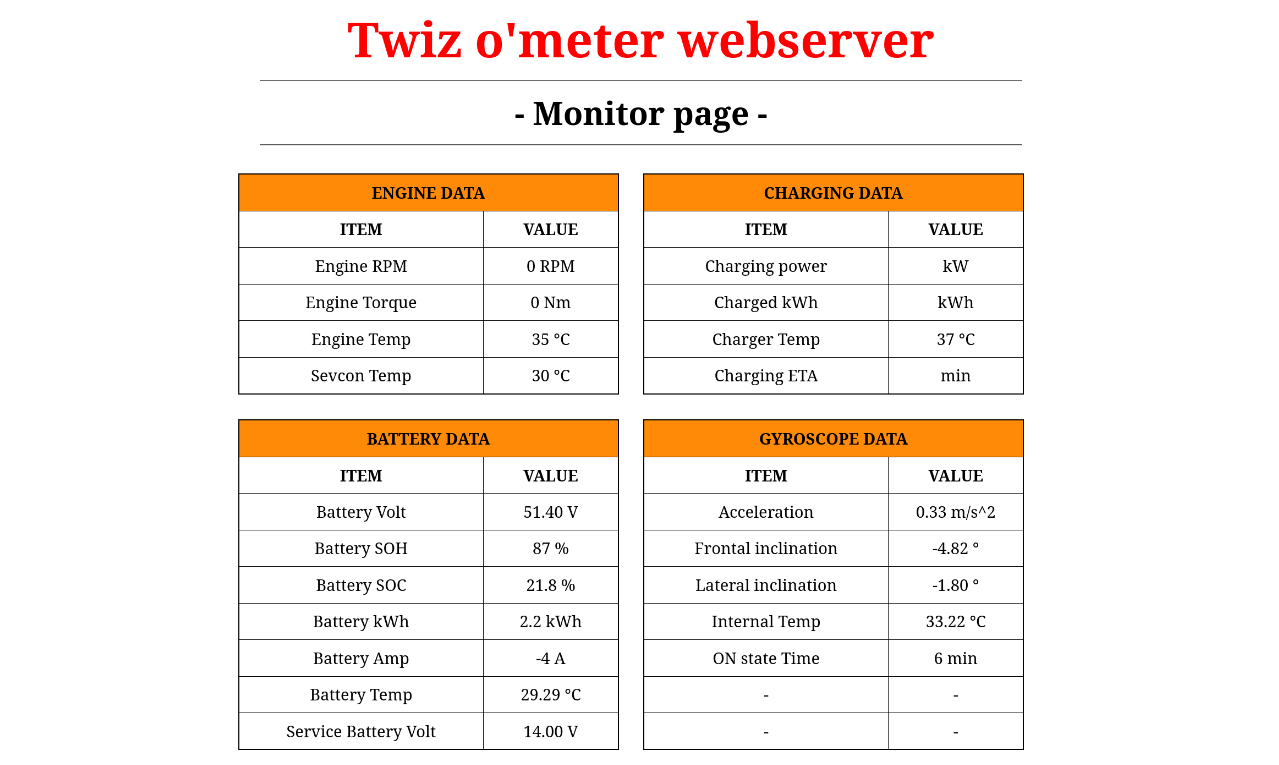
\includegraphics[width=1\textwidth]{figures/monitor_page1.png}
    \caption{Page du moniteur de données --- tableaux supérieurs.}
\end{figure}

Dans la deuxième partie de la page se trouvent les trois derniers tableaux contenant les données du tableau de bord, les données du port d'extension et le dernier réunit toutes les tensions et températures d'information de la batterie.
Appuyez sur le bouton vert \textbf{« HOME »} pointé par la flèche rouge pour revenir à la page d'accueil.

\begin{figure}[H]
    \centering
    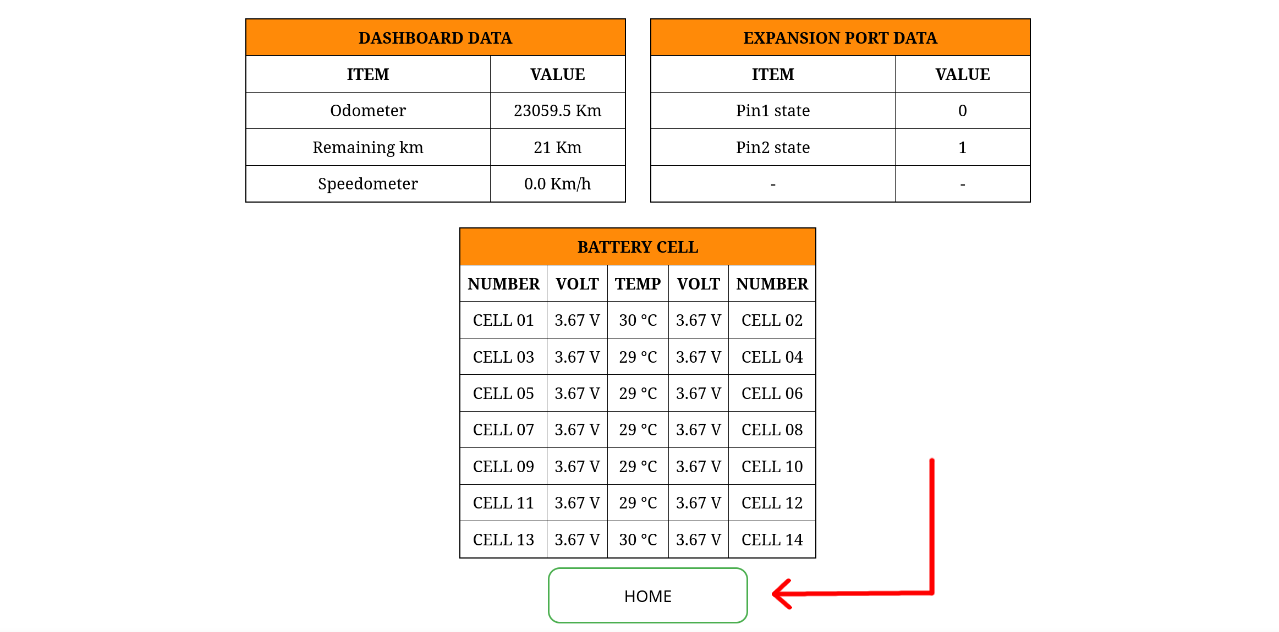
\includegraphics[width=1\textwidth]{figures/monitor_page2.png}
    \caption{Page du moniteur de données --- tableaux inférieurs.}
\end{figure}

\clearpage

\subsection{Page de l'historique des trajets}
\label{sec:web_trip_history}

Cette page contient les valeurs de la page des trajets précédemment abordée dans la Section~\ref{sec:trip_page}.
Elle peut stocker jusqu'à 5 ensembles de données différents et, même si les données affichées à l'écran sont limitées, la page du serveur web les montrera toutes. Le premier tableau présente les trajets, chacun organisé en cinq lignes, et les en-têtes de chaque enregistrement sont répertoriés dans la Section~\ref{sec:icon_list}.

\begin{figure}[H]
    \centering
    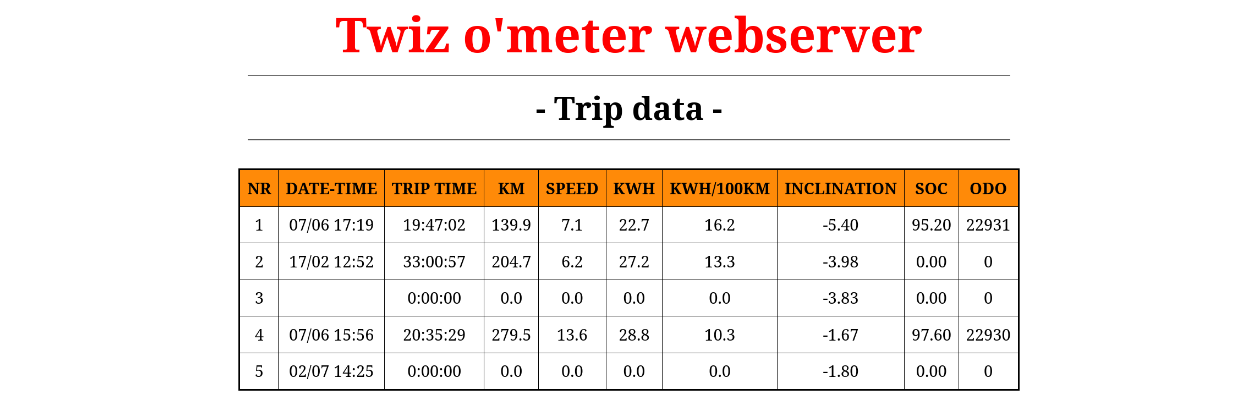
\includegraphics[width=1\textwidth]{figures/trip_page1.png}
    \caption{Page de l'historique des trajets --- Données de trajet.}
\end{figure}

Le deuxième tableau présente les vingt derniers trajets (du plus récent au plus ancien), avec les mêmes en-têtes que le premier tableau.
Vous pouvez revenir à la page de démarrage en appuyant sur le bouton vert \textbf{« HOME »} situé juste sous le deuxième tableau.

\begin{figure}[H]
    \centering
    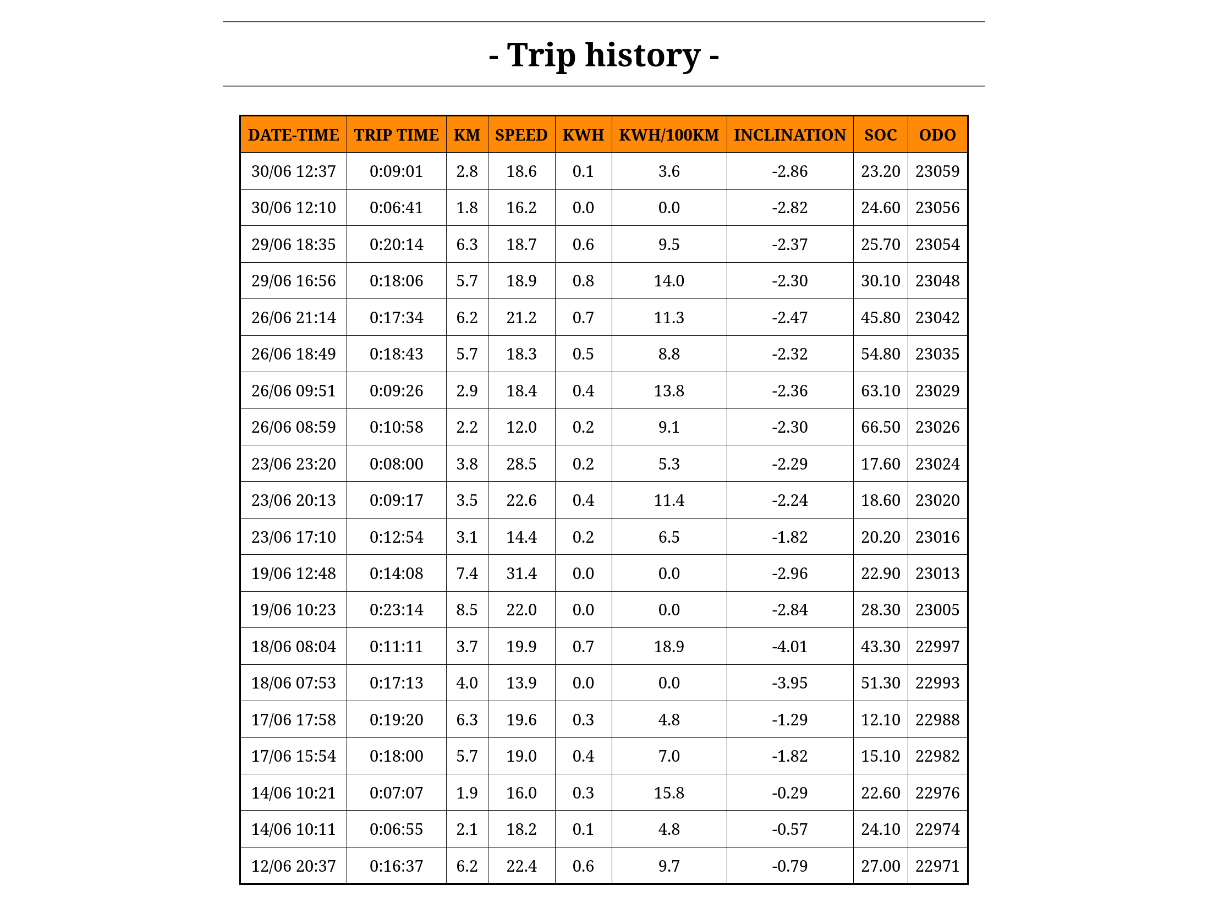
\includegraphics[width=1\textwidth]{figures/trip_page2.png}
    \caption{Page de l'historique des trajets --- Historique des trajets.}
\end{figure}


\subsection{Page des paramètres réseau}
\label{sec:web_network_settings}

Cette page vous permet de configurer les profils Wi-Fi et le broker MQTT sans avoir à utiliser le clavier de l'écran du ToM+. La page est divisée en deux tableaux principaux, l'un pour le Wi-Fi (Section~\ref{sec:wifi_settings}) et l'autre pour les paramètres MQTT (Section~\ref{sec:MQTT}).\\

Comme vous pouvez le voir sur l'image, le premier contient les quatre profils précédemment configurés sur ToM+, ou à défaut, leurs valeurs par défaut. Il en va de même pour les mots de passe, qui ne sont pas visibles jusqu'à ce que vous appuyiez sur le bouton « O » situé à côté de celui que vous souhaitez afficher. Appuyer à nouveau dessus masquera le mot de passe. 
Vous pouvez également modifier ici le mot de passe Wi-Fi du point d'accès (Section~\ref{sec:web_change_password}).

\begin{figure}[H]
    \centering
    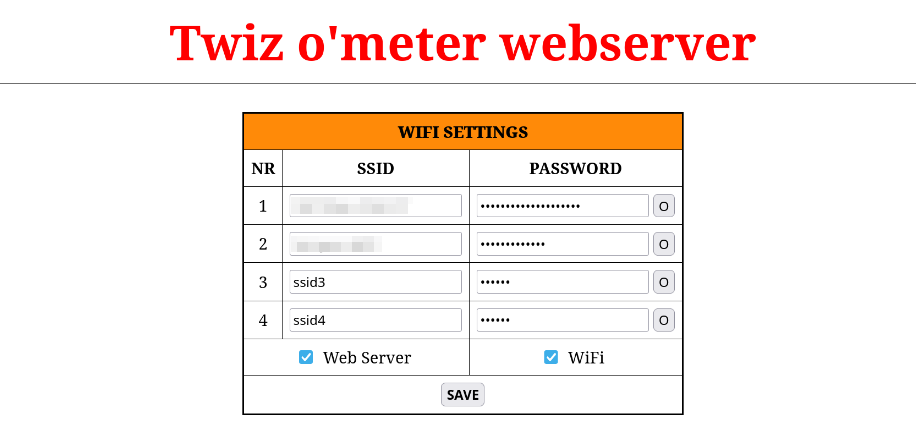
\includegraphics[width=1\textwidth]{figures/wifi_page1.png}
    \caption{Page des paramètres réseau --- Tableau Wi-Fi.}
\end{figure}

Les deux cases à cocher remplissent les mêmes fonctions que les deux curseurs de la page des paramètres Wi-Fi du ToM+. Pour savoir à quoi ils servent, reportez-vous à la Section~\ref{sec:enable_disable_wifi}.
Après toute modification, appuyez sur le bouton \textbf{« SAVE »} pour enregistrer vos changements, sinon ils seront perdus lorsque vous quitterez la page.

\begin{figure}[H]
    \centering
    
\includegraphics[width=1\textwidth]{figures/wifi_page3.png}
    \caption{Page des paramètres réseau --- Tableau du statut Wi-Fi.}
\end{figure}

Si votre ToM+ est connecté à un réseau, un petit tableau apparaîtra sous celui qui vient d'être décrit. Ses lignes contiennent trois informations principales : le SSID, l'adresse IP de ToM+ et l'adresse MAC. Ces données se trouvent également sur l'écran du ToM+, dans la page des paramètres Wi-Fi, comme montré précédemment sur la Figure~\ref{fig:wifi_bottom_line}.\\

Le second tableau principal contient les paramètres du broker MQTT tels qu'ils ont été précédemment configurés sur l'écran du ToM+, ou à défaut leurs valeurs par défaut (\textit{par ex. « broker.address »}).
Vous pouvez facilement les modifier manuellement à partir de cette page du serveur web, ce qui est beaucoup plus confortable que d'utiliser le clavier de l'écran ToM+. Découvrez ci-dessous sur l'image à quoi ce tableau peut ressembler une fois configuré.

\begin{figure}[H]
    \centering
    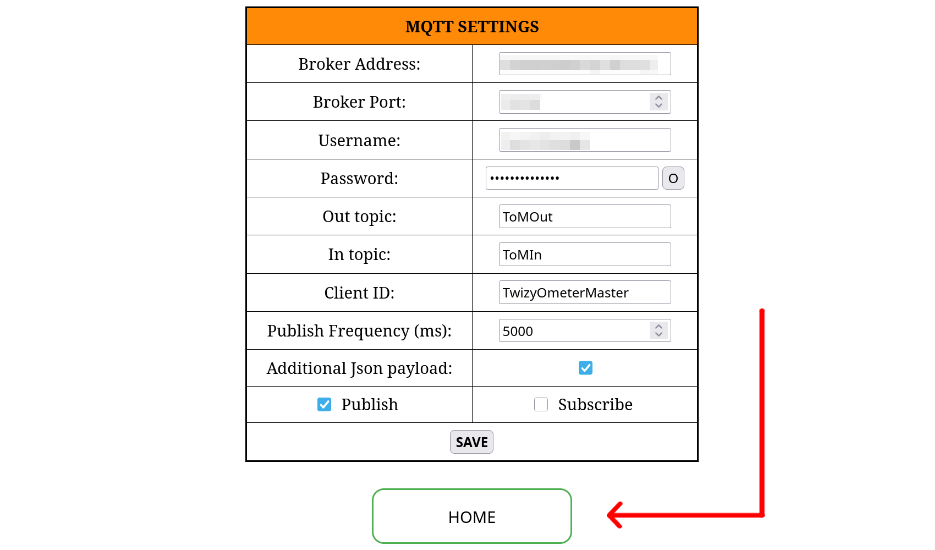
\includegraphics[width=1\textwidth]{figures/wifi_page2.png}
    \caption{Page des paramètres réseau --- Tableau MQTT.}
\end{figure}

Les deux cases à cocher remplissent les mêmes fonctions que les deux curseurs de la page des paramètres MQTT du ToM+. Pour savoir à quoi ils servent, reportez-vous à la Section~\ref{sec:enable_disable_mqtt}.
Si votre ToM+ est connecté au broker MQTT, l'en-tête du tableau affichera le texte \textbf{« (CONNECTED!) »}.\\

Après toute modification, appuyez sur le bouton \textbf{« SAVE »} pour enregistrer vos changements, sinon ils seront perdus lorsque vous quitterez la page.
Au bas de cette page, indiqué par une flèche rouge sur l'image, se trouve le bouton vert \textbf{« HOME »} pour revenir à la page d'accueil.


\subsection{Page des paramètres d'extension}
\label{sec:web_expansion_settings}

Cette page contient la configuration des broches PIN1 et PIN2 du connecteur d'extension, ainsi que la configuration du bouton du commodo d'essuie-glace droit.
Elle peut être très utile si vous aimez personnaliser des éléments et apporter votre touche personnelle à votre ToM+.
Brochage du connecteur d'extension illustré sur la Figure~\ref{fig:expansion_pinout}. 
Puisqu'il s'agit de broches d'entrée/sortie générales, vous pouvez choisir le mode de chacune selon vos besoins.\\

Si vous choisissez le mode \textbf{« INPUT »}, cette ligne écoutera le signal spécifié dans le champ suivant. Cela peut s'avérer très utile lors de la définition d'une alarme très spécifique, mais nous y reviendrons plus tard. D'autre part, si vous sélectionnez le mode \textbf{« OUTPUT »}, ToM+ transmettra le signal spécifié dans le champ suivant, qui peut être HIGH (5V) ou LOW (0V), lorsqu'une alarme se déclenche. Mais comme dit précédemment, ce point sera approfondi dans la Section~\ref{sec:web_alarm_triggers}.\\

Depuis les versions de firmware les plus récentes, de nouveaux modes autres que INPUT et OUTPUT ont été ajoutés aux broches d'extension. Découvrons-les :\\

\begin{itemize}
    \item \textbf{IR CONTROLLER} : Ce mode permet de contrôler ToM+ par une télécommande infrarouge.
    \item \textbf{KEY+ CONTROLLER} : Ce mode vous permet de contrôler votre ToM+ via une télécommande rotative à infrarouge. Pour ces deux premiers modes, un tableau de configuration supplémentaire apparaîtra.
    \item \textbf{SERIAL TX} : Permet de configurer une ligne série TX (pas encore implémentée).
    \item \textbf{SERIAL RX} : Permet de configurer une ligne série RX (pas encore implémentée).
    \item \textbf{CTRL BUTTON} : Ce mode vous permet d'utiliser le bouton du commodo d'essuie-glace droit comme bouton de commande pour les gestes de votre ToM+.
\end{itemize}

\subsubsection{Mode OUTPUT standard}

Tant en mode \textbf{« OUTPUT »} qu'en mode \textbf{« INPUT »}, vous devrez tout d'abord choisir entre \textit{« Active High »} et \textit{« Active Low »}. Lorsqu'une alarme se déclenche, un signal LOW/HIGH est envoyé à la broche choisie comme sortie d'alarme (PIN1 ou PIN2).

Si vous sélectionnez \textit{« Active High »}, le signal envoyé est HIGH (5V) et est normalement maintenu à LOW (0V).

Si vous sélectionnez \textit{« Active Low »}, le signal envoyé est LOW (0V) et est normalement maintenu à HIGH (5V).

\begin{figure}[H]
    \centering
    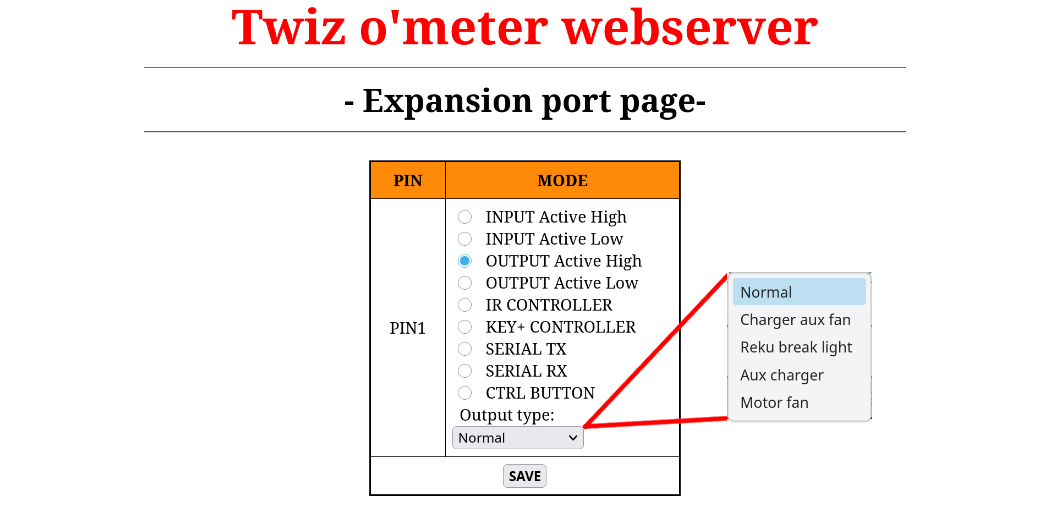
\includegraphics[width=1\textwidth]{figures/expansion_page1.png}
    \caption{Page des paramètres d'extension --- Tableau PIN1.}
\end{figure}

Comme vous pouvez le voir sur l'image ci-dessous, en sélectionnant le mode \textbf{« OUTPUT »}, vous pouvez également choisir le type de sortie \textit{« Output Type »}. C'est utile si vous avez un périphérique de sortie très spécifique nécessitant une gestion supplémentaire qui ne se limite pas au signal standard HIGH/LOW. Pour cela, vous pouvez choisir parmi une liste de périphériques de sortie déjà gérés, mis en évidence sur l'image ci-dessus.\\

Après toute modification, appuyez sur le bouton \textbf{« SAVE »} pour enregistrer vos changements, sinon ils seront perdus lorsque vous quitterez la page.
Si vous avez une idée de nouveau périphérique de sortie pouvant être utile à la communauté, n'hésitez pas à me contacter.\\

\begin{itemize}
    \item \textit{« Normal »} : C'est le mode OUTPUT standard, limité aux signaux HIGH/LOW.
    \item \textit{« Charger auxilliary fan »} : Permet de contrôler un ventilateur auxiliaire. 
    Vous devrez régler une alarme sur la température du chargeur avec un seuil. Ainsi, lors de la charge, si l'alarme se déclenche, le ventilateur commencera à refroidir le chargeur et ne s'arrêtera que lorsque la température repassera sous le seuil sélectionné avec une hystérésis fixe (même une fois la charge terminée si nécessaire).
    \item \textit{« Reku break light »} : Permet de connecter une carte relais qui contrôle les feux stop afin de les allumer en mode régénération. C'est particulièrement utile si votre Twizy est préparée pour augmenter la puissance de régénération.
    \item \textit{« Auxilliary charger »} : Permet de contrôler un chargeur auxiliaire avec une alarme sur le SOC ou la tension de batterie. Permet de connecter une carte relais qui active ou désactive un chargeur auxiliaire en cas de besoin. Il ne s'allume qu'en mode charge, avec un court délai fixe.
    \item \textit{« Motor fan »} : Permet de contrôler un ventilateur moteur avec une alarme sur la température du moteur.
    Il fonctionne de la même manière que le ventilateur du chargeur, à la différence que celui-ci ne fonctionne que pendant la conduite.
\end{itemize}

\subsubsection{Mode INPUT standard}

Comme vous pouvez le voir sur l'image ci-dessous, lors de la sélection du mode \textbf{« INPUT »}, aucun tableau supplémentaire n'apparaît.
Ce mode repose fortement sur la configuration et les déclencheurs d'alarme, veuillez donc vous référer à la Section~\ref{sec:web_alarm_triggers}.
Nous avons choisi le mode \textbf{« INPUT »} dans le second tableau, qui fonctionne de la même manière mais est destiné à la broche PIN2 du connecteur d'extension.

Après toute modification, appuyez sur le bouton \textbf{« SAVE »} pour enregistrer vos changements, sinon ils seront perdus lorsque vous quitterez la page.

\begin{figure}[H]
    \centering
    
\includegraphics[width=1\textwidth]{figures/expansion_page3.png}
    \caption{Page des paramètres d'extension --- Tableau PIN2.}
\end{figure}

\subsubsection{Mode IR CONTROLLER}

Tout d'abord, vous aurez besoin d'un récepteur IR (soit un capteur, soit un module comme celui de la première image) à brancher sur l'une des broches de la carte d'extension.
Ce mode est destiné à être utilisé avec une télécommande IR générique, mais celle que je suggère personnellement est celle montrée sur la deuxième image ci-dessous, spécialement conçue pour être installée sur le volant.

\begin{figure}[ht]
    \centering

    \begin{subfigure}[t]{0.48\textwidth}
        \centering
        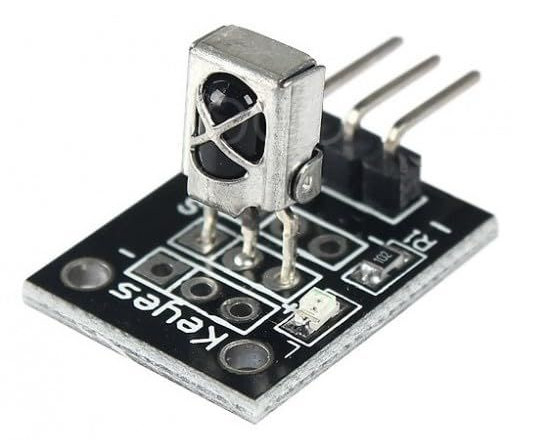
\includegraphics[width=\linewidth]{figures/ir_receiver.jpg}
        \caption{Module récepteur IR.}
    \end{subfigure}
    \hfill
    \begin{subfigure}[t]{0.48\textwidth}
        \centering
        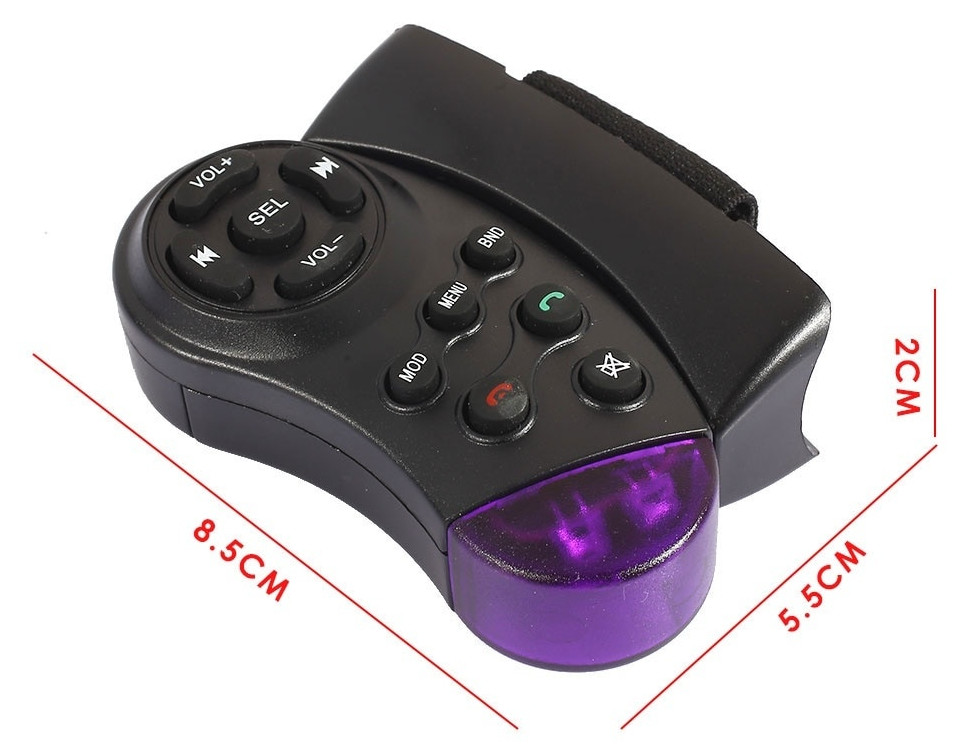
\includegraphics[width=\linewidth]{figures/ir_controller_photo.jpg}
        \caption{Télécommande IR de volant.}
    \end{subfigure}
\end{figure}

Lorsque vous sélectionnez le mode \textbf{« IR CONTROLLER »} pour le tableau de la broche PIN1 ou PIN2, n'oubliez pas d'appuyer sur le bouton \textbf{« SAVE »} pour enregistrer vos modifications. Une fois enregistré, la page se rechargera et un tableau supplémentaire apparaîtra en dessous, visible sur l'image ci-dessous.

\begin{figure}[H]
    \centering
    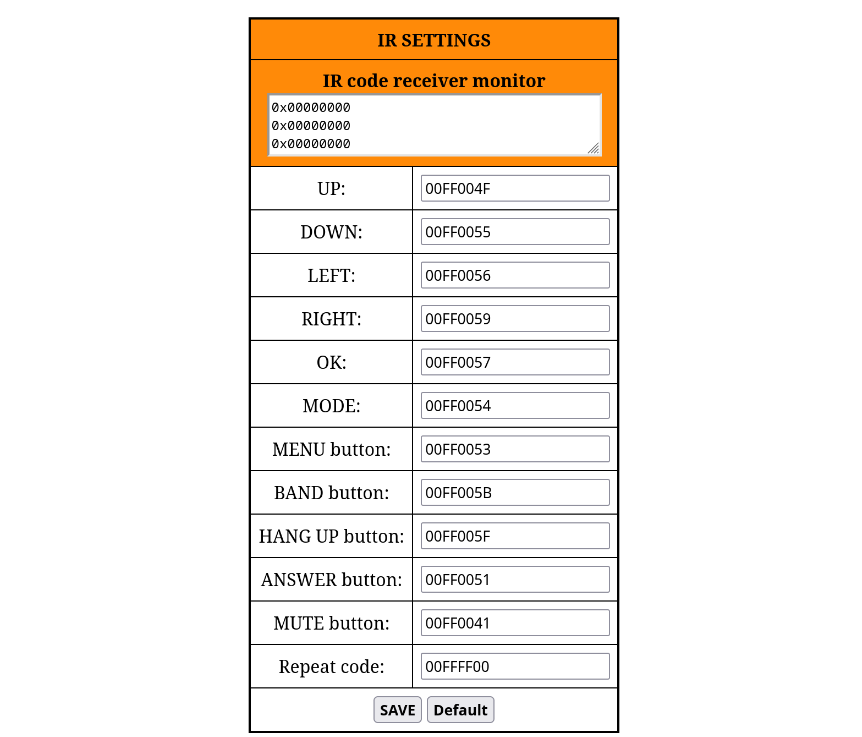
\includegraphics[width=0.8\textwidth]{figures/ir_settings.png}
    \caption{Page des paramètres d'extension --- Tableau des réglages IR.}
\end{figure}

Ce tableau vous aidera à associer chaque bouton de la télécommande IR avec le code IR correspondant.
Dans la partie supérieure du tableau, il y a une zone de texte que vous pouvez utiliser comme \textbf{moniteur de récepteur de code IR} pour tester en temps réel les codes IR de votre télécommande après avoir branché le récepteur IR.\\

Grâce à cela, vous pouvez remplir les autres champs en conséquence. Le dernier est particulièrement important : c'est le code que la télécommande envoie lorsque vous maintenez un bouton enfoncé.
Ensuite, n'oubliez pas d'appuyer sur le bouton \textbf{« SAVE »} pour enregistrer vos modifications, sinon elles seront perdues en quittant la page.
Enfin, un bouton pratique \textbf{« Default »} est situé à côté pour rétablir facilement vos modifications si nécessaire.

\subsubsection{Mode KEY+ CONTROLLER}

Ce mode est très similaire à celui qu'on vient de décrire, mais il est destiné à être utilisé avec un autre type de commande (celui présenté sur la photo ci-dessous). Il s'agit d'une commande rotative sans fil Bluetooth pour systèmes audio embarqués, qui effectue différentes actions en fonction de la vitesse à laquelle vous tournez la bague externe. Et bien sûr, elle possède aussi d'autres boutons sur la partie interne.\\

\begin{figure}[H]
    \centering
    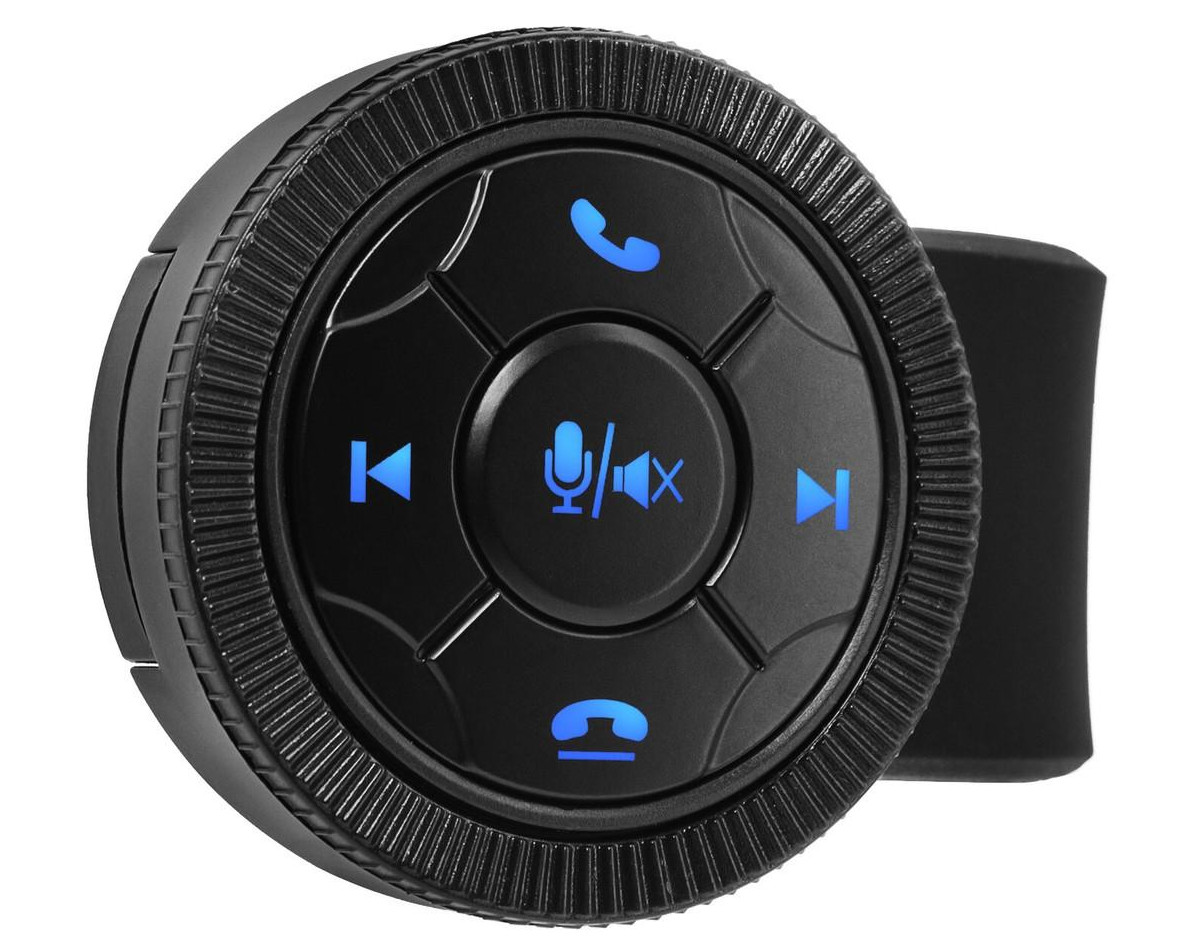
\includegraphics[width=0.4\textwidth]{figures/keyp_controller.jpg}
    \caption{Commande rotative sans fil Bluetooth.}
\end{figure}

Lorsque vous sélectionnez le mode \textbf{« KEY+ CONTROLLER »} pour le tableau PIN1 ou PIN2, pensez à appuyer sur le bouton \textbf{« SAVE »} pour enregistrer vos modifications. Une fois enregistré, la page se rechargera et un tableau supplémentaire apparaîtra ci-dessous, vous pouvez le voir sur l'image ci-dessous.

\begin{figure}[H]
    \centering
    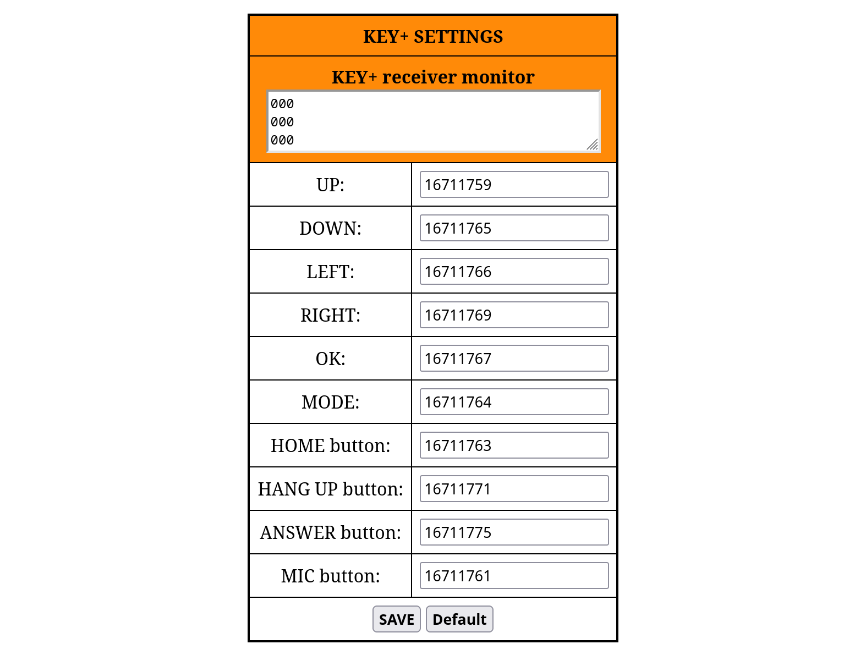
\includegraphics[width=0.8\textwidth]{figures/keyp_settings.png}
    \caption{Page des paramètres d'extension --- Tableau des réglages KEY+.}
\end{figure}

Cela fonctionne de la même manière que le tableau des paramètres IR. La différence majeure réside dans ce que ToM+ lit depuis le port d'extension : il ne s'agit plus d'un code IR, mais d'une tension.

Dans l'image ci-dessus sont affichées les valeurs par défaut, allant de \textit{0} à \textit{3.3V} écrites sans la virgule décimale. Par exemple, \textit{018} signifie \textit{0.18V} et \textit{157} signifie \textit{1.57V}, et ainsi de suite.
ToM+ a une tolérance de \textit{0.05V} sur les valeurs d'entrée afin d'éviter les rebonds de tension.\\

Après cela, n'oubliez pas d'appuyer sur le bouton \textbf{« SAVE »} pour enregistrer vos modifications, sinon elles seront perdues quand vous quittiez la page. Enfin, un bouton utile \textbf{« Default »} est situé juste à côté pour annuler facilement vos changements au besoin.

\subsubsection{Mode CTRL BUTTON}
\label{sec:web_wiper_stalk}

Ce dernier tableau contient la configuration nécessaire pour faire fonctionner le \textbf{bouton du commodo d'essuie-glace droit} fourni (Figure~\ref{fig:wiper_stalk_button}).
Vous pouvez utiliser ce bouton pour naviguer dans toute l'interface ToM+ sans utiliser l'écran tactile, grâce à ces trois \textbf{actions} principales : \textit{« Browse items »} (Parcourir les éléments), \textit{« Change page »} (Changer de page), \textit{« Select-deselect »} (Sélectionner-désélectionner).
Pour ce faire, il existe trois types d'\textbf{appuis sur le bouton} : \textit{« Short »} (Court), \textit{« Medium »} (Moyen), \textit{« Long »} (Long).\\

\begin{figure}[H]
    \centering
    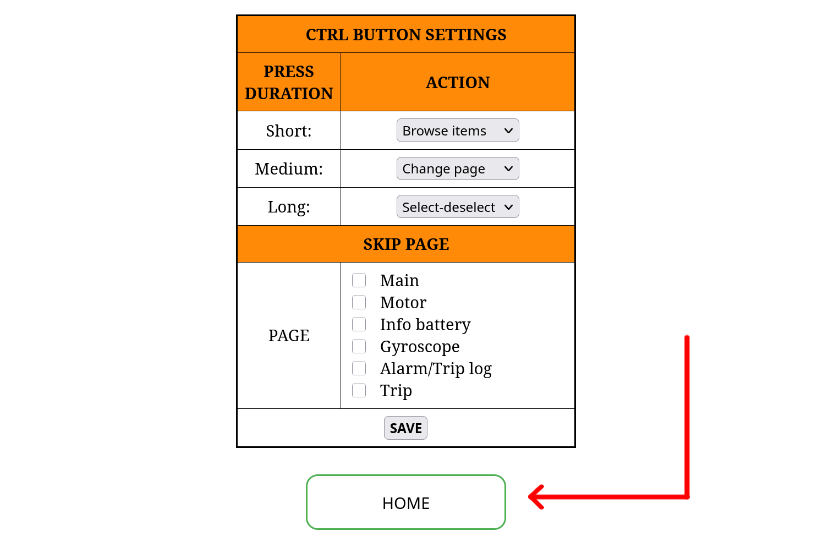
\includegraphics[width=1\textwidth]{figures/expansion_page2.png}
    \caption{Page des paramètres d'extension --- Tableau du bouton d'essuie-glace.}
\end{figure}

Ainsi, dans la première partie de ce tableau, vous pouvez réorganiser ces actions avec les gestes de votre choix.\\

\begin{itemize}
    \item \textit{« Browse items »} : Déplace un petit marqueur blanc à côté de la donnée actuellement sélectionnée.
    \item \textit{« Change page »} : Permet de faire défiler les pages présentes dans la boucle.
    \item \textit{« Select-deselect »} : Simule un appui sur la donnée sélectionnée (ex. passe de l'arrière-plan au premier plan).\\
\end{itemize}

Dans la deuxième partie du tableau, vous pouvez sélectionner les \textbf{pages que vous souhaitez ignorer} lors du défilement des pages disponibles en répétant le geste \textit{« Change page »}. Par exemple, si je ne souhaite pas surveiller la page d'info batterie lors du défilement avec le bouton, il me suffit de la décocher pour qu'elle soit retirée de la boucle.\\

Après toute modification, appuyez sur le bouton \textbf{« SAVE »} pour enregistrer vos changements, sinon ils seront perdus lorsque vous quitterez la page.
Au bas de cette page, indiqué par une flèche rouge sur l'image, se trouve le bouton vert \textbf{« HOME »} pour revenir à la page d'accueil.

\clearpage

\subsection{Page des déclencheurs d'alarme}
\label{sec:web_alarm_triggers}

Lorsque quelque chose se produit sur ToM+ et que vous souhaitez en être notifié, vous pouvez choisir comment être averti et quand dans cette page. Vous pouvez avoir jusqu'à \textbf{dix alarmes} fonctionnant simultanément et ToM+ vérifie en permanence l'état de chaque condition.
L'image montre le premier tableau, où vous pouvez voir les alarmes actuellement actives.

\begin{figure}[H]
    \centering
    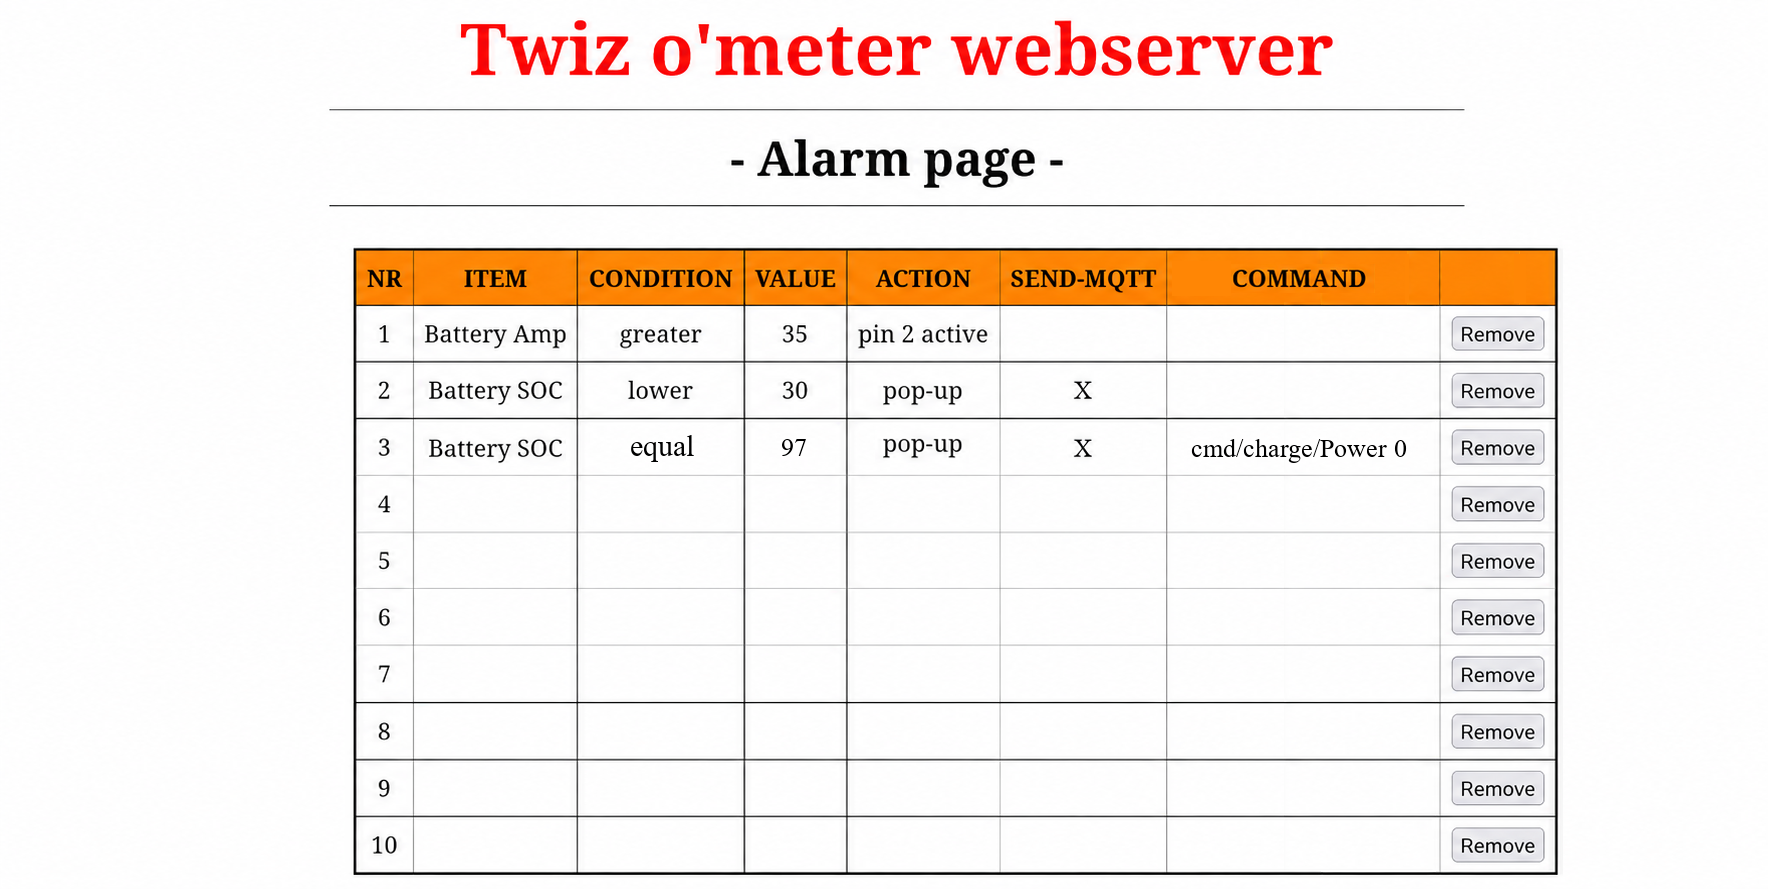
\includegraphics[width=1\textwidth]{figures/alarm_page1.png}
    \caption{Page d'alarme --- Tableau de la liste des alarmes existantes.}
\end{figure}

Les en-têtes des tableaux sont concrètement les éléments de la condition écoutés par ToM+.\\

\begin{itemize}
    \item \textbf{ITEM} : C'est la donnée à vérifier, choisie dans la liste de la Section~\ref{sec:icon_list}.
    \item \textbf{CONDITION} : C'est le signe opérateur utilisé lors de la comparaison des valeurs.
    \item \textbf{VALUE} : C'est une valeur entière signée utilisée comme second terme de la comparaison.
    \item \textbf{ACTION} : C'est l'action exécutée lorsque l'alarme se déclenche. Voir le tableau suivant.
    \item \textbf{SEND-MQTT} : C me champ binaire et, s'il est coché, publie un message sur le topic MQTT.
    \item \textbf{COMMAND} : C'est une chaîne de caractères facultative à envoyer en tant que commande supplémentaire.
\end{itemize}
\  \\
Le premier déclencheur d'alarme vérifie la consommation de la batterie et active la broche PIN2 de la carte d'extension si elle est supérieure à 35A. Dans cet exemple spécifique, il sert à allumer le feu stop arrière lorsque la régénération est suffisante pour faire ralentir la Twizy.\\

Le deuxième déclencheur d'alarme vérifie le SOC de la batterie et affiche sur l'écran une simple fenêtre contextuelle notifiant que le niveau de batterie est inférieur à 30 \%. En cochant le champ \textit{« Change page »}, j'ai ajouté une option supplémentaire qui demandera à ToM+ d'envoyer un message MQTT lorsque cette alarme se déclenche.\\

Le troisième déclencheur d'alarme vérifie le SOC de la batterie et une fois la charge terminée (par exemple égale à 97 \%), il fait la même chose qu'auparavant mais exécute une commande supplémentaire. La commande \textit{cmd/charge/Power 0} désactive un interrupteur Wi-Fi Tasmota qui relie la prise de la Twizy à la prise murale.

La fonction de la colonne \textbf{« COMMAND »} est donc très utile et vous permet d'intégrer votre ToM+ dans votre maison connectée. Consultez l'Annexe~\ref{apx:tasmota} pour des configurations détaillées.\\

Lorsque vous souhaitez supprimer une alarme spécifique, il vous suffit d'appuyer sur le bouton \textbf{« Remove »} dans sa dernière colonne.\\


\begin{figure}[H]
    \centering
    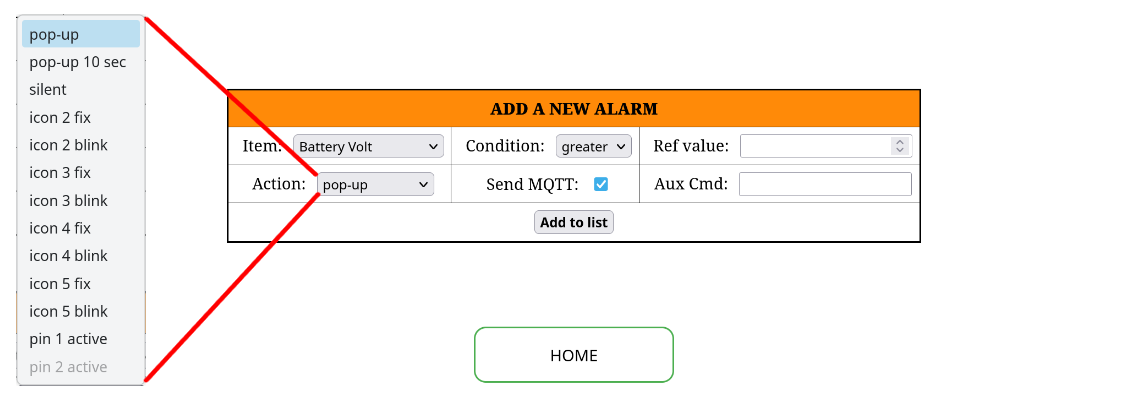
\includegraphics[width=1\textwidth]{figures/alarm_page2.png}
    \caption{Page d'alarme --- Tableau d'ajout d'une nouvelle alarme.}
\end{figure}

Dans le deuxième tableau, vous pouvez ajouter une nouvelle alarme à la liste qu'on vient d'évoquer.
Tout d'abord, vous devez choisir l'\textbf{ITEM}, parmi toutes les données disponibles listées dans la Section~\ref{sec:icon_list}.
Dans cette zone de choix, les éléments sont organisés comme dans la liste citée.
Sélectionnez ensuite la \textbf{CONDITION}, c'est-à-dire l'opérateur de la comparaison, entre \textit{« lower »} (inférieur), \textit{« greater »} (supérieur) ou \textit{« equal »} (égal).
Vient ensuite le moment de saisir la valeur de référence \textbf{VALUE}, un nombre entier signé qui constitue le terme de droite de la comparaison.\\

Prenons le temps d'expliquer toutes les \textbf{ACTION}s possibles.\\

\begin{itemize}
    \item \textit{pop-up} : une fenêtre contextuelle jaune notifiant la valeur de l'élément apparaît au centre de l'écran. Pour la masquer, appuyez dessus une fois. Vous pouvez voir un exemple de pop-up sur la première image ci-dessous.
    \item \textit{pop-up 10 sec} : une fenêtre pop-up jaune notifiant la valeur de l'élément reste à l'écran pendant dix secondes.
    \item \textit{silent} : aucune action visible n'a lieu : c'est généralement utilisé uniquement pour publier des messages MQTT.
    \item \textit{icon x fix} : l'icône x (\textit{où x peut être 2, 3, 4 ou 5}) s'allume. Voir la Figure~\ref{fig:alarm_icons2} pour les icônes d'alarme.
    \item \textit{icon x blink} : l'icône x (\textit{où x peut être 2, 3, 4 ou 5}) commence à clignoter.
    \item \textit{pin1 active} : la broche PIN1 de la carte d'extension s'active (LOW ou HIGH selon le niveau sélectionné sur la page des paramètres d'extension dans la Section~\ref{sec:web_alarm_triggers}).
    \item \textit{pin2 active} : la broche PIN2 de la carte d'extension s'active. Dans cet exemple, PIN2 a été configurée en mode INPUT, elle est donc grisée car elle ne peut pas représenter une action OUTPUT.
\end{itemize}
\  \\
\begin{figure}[ht]
    \centering

    \begin{subfigure}[t]{0.48\textwidth}
        \centering
        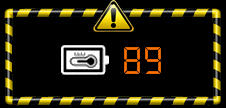
\includegraphics[width=\linewidth]{figures/pop-up.PNG}
        \caption{Pop-up : Température batterie > 89°C.}
    \end{subfigure}
    \hfill
    \begin{subfigure}[t]{0.48\textwidth}
        \centering
        
\includegraphics[width=\linewidth]{figures/alarm_icons.png}
        \caption{Icônes d'alarme (2, 3, 4 et 5).}\label{fig:alarm_icons2}
    \end{subfigure}
\end{figure}

Le champ suivant est le drapeau binaire \textbf{SEND MQTT} : s'il est activé, ToM+ publie un message MQTT sur le topic OUT MQTT configuré (ex. TOMout, voir Section~\ref{sec:mqtt_connection}) lorsque l'alarme se déclenche en guise de notification supplémentaire. Enfin, le champ texte \textbf{AUX CMD} contient une commande supplémentaire à envoyer via MQTT à d'autres appareils IoT.
Voir l'Annexe~\ref{apx:tasmota} pour les configurations détaillées d'un interrupteur Tasmota à titre d'exemple.\\

Enfin, vous pouvez ajouter votre alarme en appuyant sur le bouton \textbf{« Add to list »}. La page se recharge automatiquement et le déclencheur d'alarme est ajouté à la liste du premier tableau.

Appuyez sur le bouton vert \textbf{« HOME »} en bas de la page pour revenir à la page d'accueil.


\subsection{Page du journal des alarmes}
\label{sec:web_alarms_log}

Cette page enregistre les 21 derniers déclenchements d'alarme et remplit la même fonction que la page de journal de ToM, comme présenté dans la Section~\ref{sec:alarm_log}. Vous pouvez également consulter et supprimer tout enregistrement indésirable en appuyant sur le bouton \textbf{« Remove »} situé près de celui que vous souhaitez supprimer définitivement (sur l'écran ToM+ également).\\

\begin{figure}[H]
    \centering
    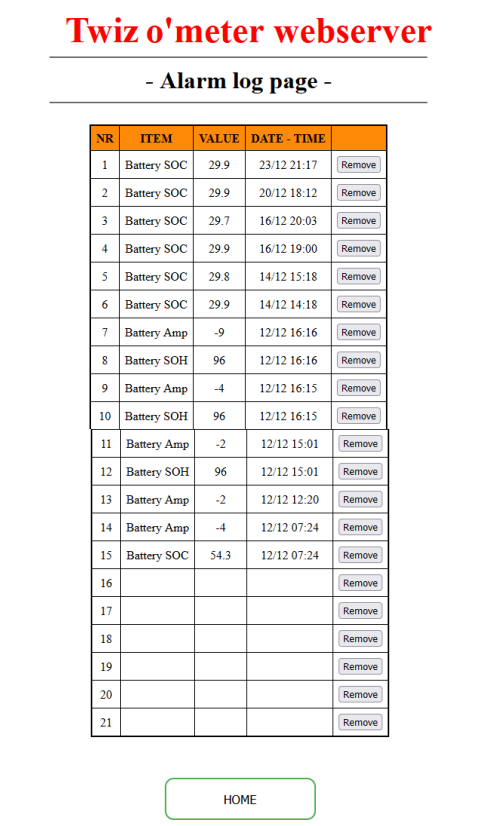
\includegraphics[width=0.6\textwidth]{figures/alarm_log1.png}
    \caption{Tableau de la page du journal des alarmes.}
\end{figure}

Évidemment, le tableau contient l'\textbf{ITEM} et la valeur \textbf{VALUE} qui ont déclenché l'alarme.
Des champs supplémentaires indiquent également la date et l'heure auxquelles le déclenchement s'est produit.
Ensuite, comme d'habitude, appuyez sur le bouton vert \textbf{« HOME »} en bas de page pour revenir à la page d'accueil.


\subsection{Page des mises à jour OTA \& Préférences}
\label{sec:web_ota_update}

Dans cette page, vous pouvez \textbf{mettre à jour le firmware} à la volée depuis l'interface web, sans avoir à vous battre avec l'outil de flashage comme sur les anciennes versions. Cette nouvelle fonctionnalité fait gagner du temps et s'avère bien plus conviviale : veillez donc à toujours avoir la dernière version du firmware installée pour accéder aux fonctionnalités et améliorations les plus récentes !

\subsubsection{Mise à jour OTA}

Le premier tableau vous donne des informations sur le firmware du boîtier noir (blackbox) : analysons ces valeurs. Le \textbf{ESP fw} est probablement l'élément le plus important de la grille car il vous indique la version actuellement installée et chargée sur la carte mère ESP.

Un autre champ utile est le \textbf{S/N} qui signifie numéro de série (Serial Number), que vous pouvez également trouver sur ToM+ comme vu sur la Figure~\ref{fig:settings_page}. La ligne suivante est un peu plus technique et est directement liée au mécanisme de mise à jour OTA (Over-The-Air).
\textbf{Current ptn} et \textbf{Next ptn} font référence aux adresses de partition où le firmware est actuellement stocké et où il sera stocké pendant que la mise à jour est en cours.\\

Parfois, des correctifs de firmware (comme des corrections de bugs ou des ajustements mineurs) peuvent être publiés sans changer le numéro de version (ex. 2.4). Dans ces cas-là, il peut être utile de connaître le fichier binaire spécifique installé, c'est pourquoi les deux champs suivants contiennent son nom complet.
Comme vous pouvez le constater, il existe deux partitions principales de firmware, \textbf{Ota0} et \textbf{Ota1}, afin que vous puissiez avoir deux versions différentes installées et passer de l'une à l'autre au besoin.
Ici, le nom complet est \textit{ESP32\_Fw24\_70\_4error12} pour les deux.

Le dernier champ correspond au nom complet du firmware de la \textbf{Special partition}, qui est un stockage supplémentaire utilisé pour accueillir des logiciels tiers (ex. le logiciel de réglage Twizy-cfg).
Pour plus d'informations sur la modification de votre Twizy avec Twizy-cfg sur ToM+, reportez-vous à l'Annexe~\ref{apx:tuning}.

\begin{figure}[H]
    \centering
    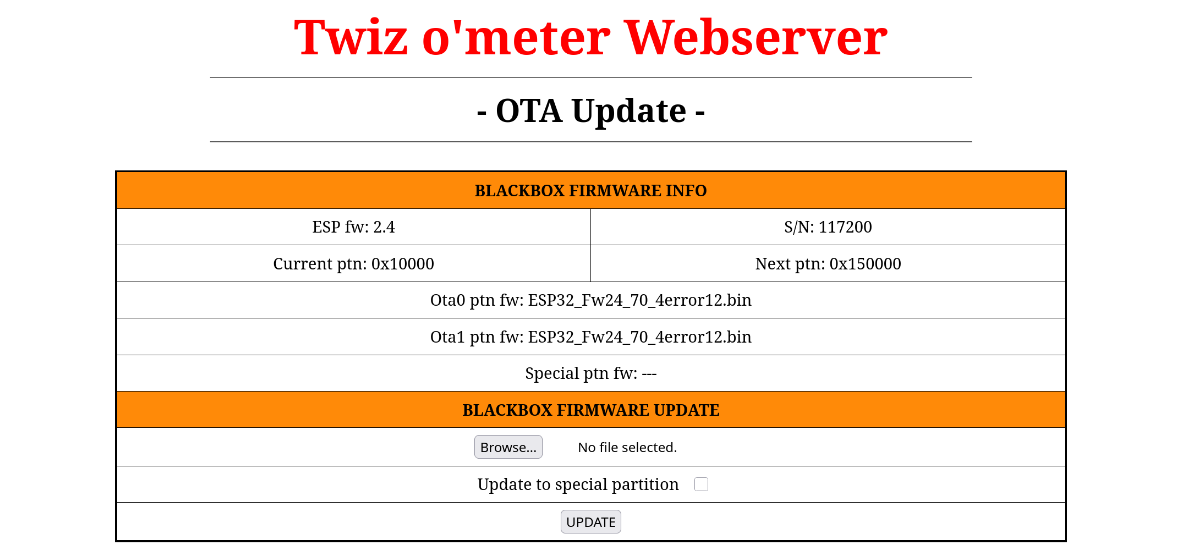
\includegraphics[width=1\textwidth]{figures/ota_page3.png}
    \caption{Page de mise à jour OTA --- Tableau de mise à jour et d'informations.}
\end{figure}

La deuxième partie de ce tableau vous permet de mettre à jour le firmware ou de charger un logiciel tiers. Tout d'abord, téléchargez le fichier binaire (avec l'extension .bin) que vous souhaitez installer sur ToM+. Appuyez ensuite sur le bouton \textbf{« Browse\ldots »} et parcourez les dossiers de votre appareil jusqu'à trouver le fichier désiré.

S'il s'agit d'une \textit{mise à jour ToM+ standard}, appuyez directement sur le bouton \textbf{« UPDATE »}. Pour suivre l'avancement de la mise à jour, une barre de progression orange apparaît en bas du tableau avec son pourcentage. Lorsqu'elle atteint 100 \%, ToM+ redémarrera pour appliquer les modifications.

S'il s'agit d'un \textit{logiciel tiers}, veillez à cocher l'option \textit{« Update to special partition »} et, seulement après cela, appuyez sur le bouton \textbf{« UPDATE »}. Dès que la mise à jour est terminée, ToM+ redémarre et charge le firmware de la partition spéciale.\\

Dans le tableau \textbf{« BOOT OPTIONS »}, une fois les firmwares souhaités chargés, vous pouvez basculer de l'un à l'autre en cas de besoin. Admettons que j'exécute le firmware ToM+ 2.4 et que je souhaite faire des réglages avec le logiciel tiers Twizy-cfg ; j'ai déjà chargé les deux dans les partitions appropriées. Pour ce faire, appuyez sur le bouton \textit{« Reboot from special partition »} et attendez que ToM+ redémarre, puis suivez l'Annexe~\ref{apx:tuning} pour la suite.\\

Les boutons \textit{« Reboot from Ota0 partition »} et \textit{« Reboot from Ota1 partition »} permettent de basculer entre les versions du firmware ToM+. Supposons que j'utilise le firmware ToM+ 2.4 mais que, pour une raison quelconque, je souhaite revenir à la version 2.3 que j'avais auparavant. Pour cela, appuyez sur le bouton correspondant pour redémarrer depuis Ota1 ou Ota0. ToM+ redémarrera immédiatement et vous serez déconnecté de l'interface web.

\begin{figure}[H]
    \centering
    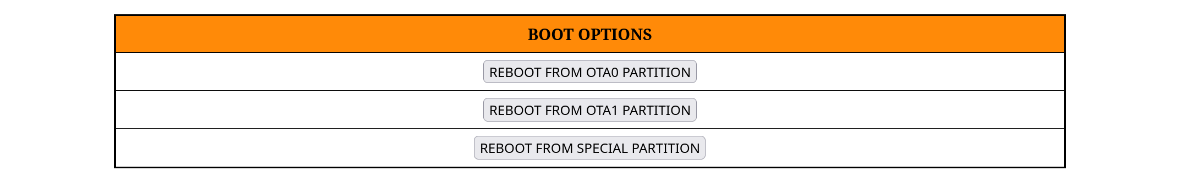
\includegraphics[width=1\textwidth]{figures/ota_boot.png}
    \caption{Page de mise à jour OTA --- Tableau des options de démarrage.}
\end{figure}

En passant au tableau suivant, nous avons le tableau \textbf{« LCD FIRMWARE UPDATE »}, qui permet également d'effectuer des mises à jour OTA pour l'écran LCD. Cela signifie qu'il n'y a plus besoin de s'embêter avec la carte microSD et le petit trou sur l'écran.\\

\textbf{AVERTISSEMENT :} Comme indiqué dans le tableau, vous \textbf{NE DEVEZ PAS} fermer cette page web pendant la mise à jour : il est conseillé de désactiver votre écran de veille pour éviter tout échec de la mise à jour. Le processus peut prendre quelques minutes, selon la version du firmware, jusqu'à 10 minutes.\\

La procédure est similaire à la mise à jour OTA du boîtier noir. Tout d'abord, téléchargez le fichier (avec l'extension .tft) que vous souhaitez installer sur ToM+. Appuyez ensuite sur le bouton \textbf{« Browse\ldots »} et parcourez les dossiers de votre appareil pour trouver le fichier souhaité.

Si vous \textit{mettez à jour l'écran principal}, appuyez sur le bouton \textbf{« UPDATE LCD »}.
Pour suivre l'état de la mise à jour, la barre de progression bleue sous l'encadré d'avertissement affichera les blocs copiés vers l'écran LCD. Lorsqu'elle sera terminée, l'écran redémarrera (et non le boîtier noir).

Si vous \textit{mettez à jour l'écran secondaire (twin display)}, veillez à cocher l'option \textit{« Update AUX LCD »} et, seulement après, appuyez sur le bouton \textbf{« UPDATE LCD »}. Dès que la mise à jour est terminée, l'écran LCD redémarre et charge le firmware souhaité.

\begin{figure}[H]
    \centering
    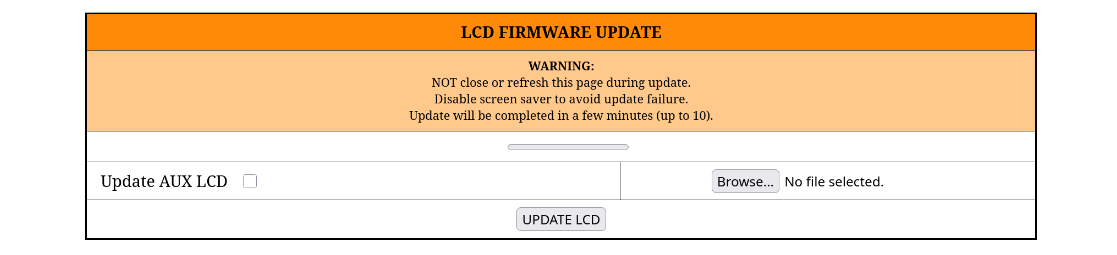
\includegraphics[width=1\textwidth]{figures/ota_lcd.png}
    \caption{Page de mise à jour OTA --- Tableau de mise à jour du firmware LCD.}
\end{figure}


\subsubsection{Préférences et mise à niveau matérielle}

Dans la section suivante de la page web, nous pouvons gérer les préférences, ce qui inclut les configurations Wi-Fi et MQTT, l'organisation des icônes de pages ToM+, et bien plus encore. Il est donc toujours conseillé d'effectuer une \textbf{sauvegarde avant de mettre à jour}, afin d'éviter de devoir ressaisir vos mots de passe si une mise à jour se passe mal. Pour ce faire, appuyez sur le bouton \textbf{« BACKUP »} et un fichier nommé \textit{prefs.ToM} sera téléchargé sur votre appareil. Parfois, une fenêtre pop-up s'ouvre pour vous avertir que ce fichier a une extension inhabituelle : cliquez sur le bouton \textit{Conserver} et téléchargez-le quand même.\\

Le processus inverse est tout aussi simple. Appuyez sur le bouton \textbf{« Browse\ldots »} et parcourez les dossiers de votre appareil jusqu'à trouver le fichier de préférences \textit{prefs.ToM}. Pour appliquer les modifications, appuyez sur le bouton \textbf{« RESTORE »} et vous serez réorienté vers la page d'accueil pour confirmation.

\begin{figure}[H]
    \centering
    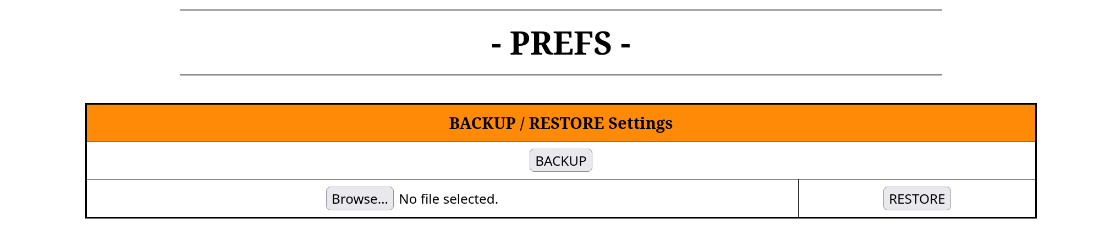
\includegraphics[width=1\textwidth]{figures/prefs_page.png}
    \caption{Page de mise à jour OTA --- Tableau de sauvegarde des préférences.}
\end{figure}

Ce tableau suivant est très spécifique aux utilisateurs des anciennes versions de ToM qui ont maintenant reçu le mot de passe pour mettre à niveau leur appareil vers ToM+ sans changer le boîtier noir. Si c'est votre cas, veuillez saisir le mot de passe dans le champ texte et appuyer sur le bouton \textbf{« UPGRADE »}.
Dès lors, votre ToM est enfin mis à niveau vers ToM+, profitez-en !

\begin{figure}[H]
    \centering
    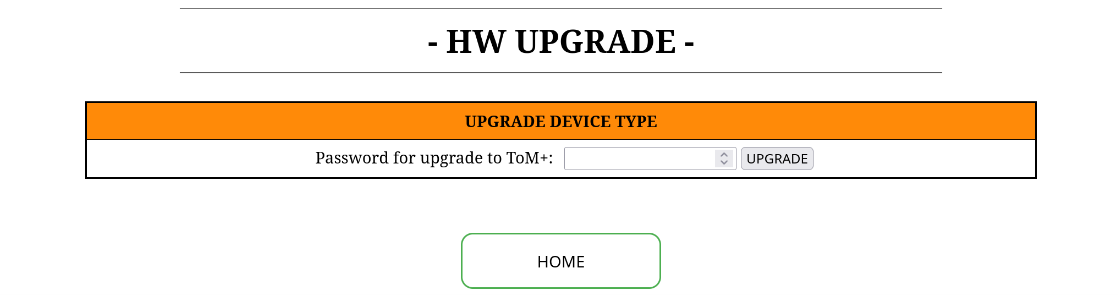
\includegraphics[width=1\textwidth]{figures/hw_upgrade.png}
    \caption{Page de mise à jour OTA --- Tableau de mise à niveau matérielle.}
\end{figure}

Appuyez sur le bouton vert \textbf{« HOME »} en bas du tableau pour revenir à la page d'accueil.

\clearpage

\subsection{Page des infos et réglages avancés}
\label{sec:web_advanced_info}

Cette page est destinée à divers réglages avancés qui ne sont pas disponibles dans les pages de paramètres d'affichage du ToM+ abordées dans la Section~\ref{sec:settings_page} pour des raisons d'espace.\\

La première case, \textbf{« Disable Auto-dimming »}, peut être cochée si vous ne souhaitez pas que l'écran LCD de ToM+ adapte sa luminosité lors de l'allumage des feux.
Sinon, vous pouvez régler la luminosité de variation \textbf{« Dimming brightness (\%) »} exprimée en pourcentage (jusqu'à 100 \%), et définir vous-même le facteur de réduction de luminosité lorsque les feux sont activés.

\begin{figure}[H]
    \centering
    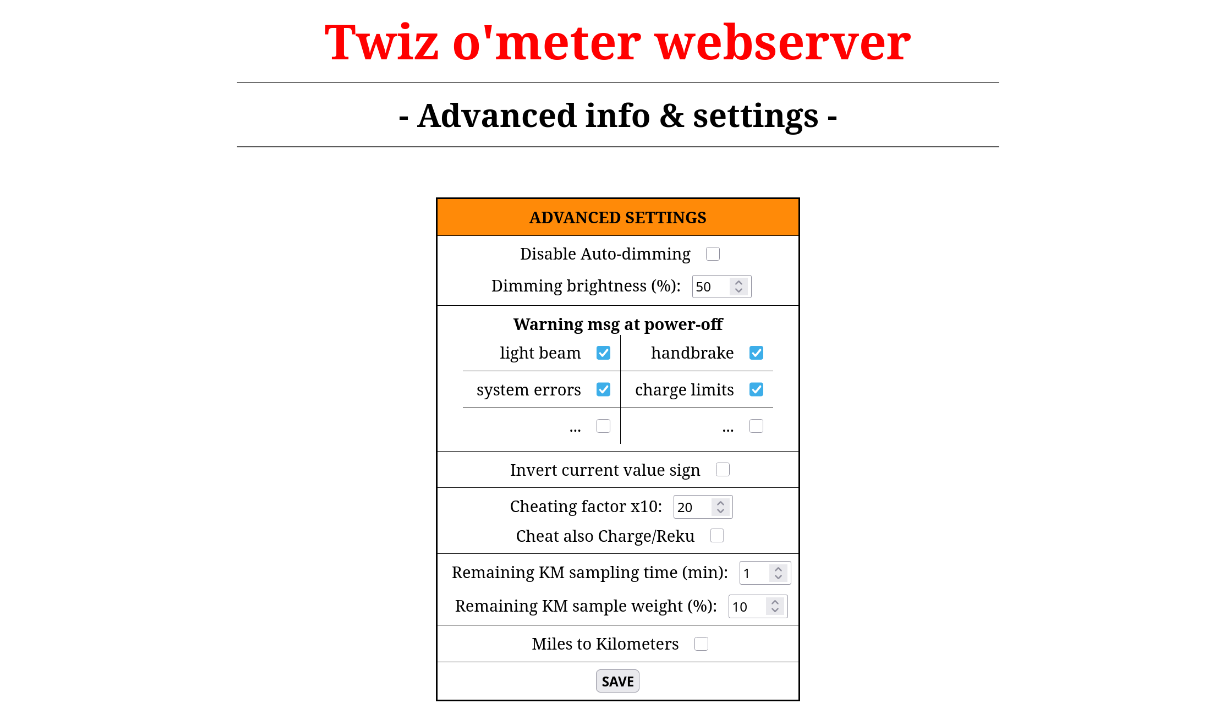
\includegraphics[width=1\textwidth]{figures/adv_sett_page1.png}
    \caption{Page des infos avancées --- Tableau des paramètres avancés.}
\end{figure}

Ensuite, nous trouvons la sous-section \textbf{Warning messages at power-off} (messages d'avertissement à l'extinction), où vous pouvez sélectionner les rappels (\textit{feux} et \textit{frein à main}) et informations (\textit{erreurs système} et \textit{limites de charge}) affichés sur la fenêtre pop-up d'extinction de ToM+. Cela ressemble à l'image ci-dessous, vous informant par exemple si vous avez oublié d'engager le frein à main.
Les deux dernières cases à cocher sont réservées à des usages futurs et ne sont pas encore implémentées.

\begin{figure}[H]
    \centering
    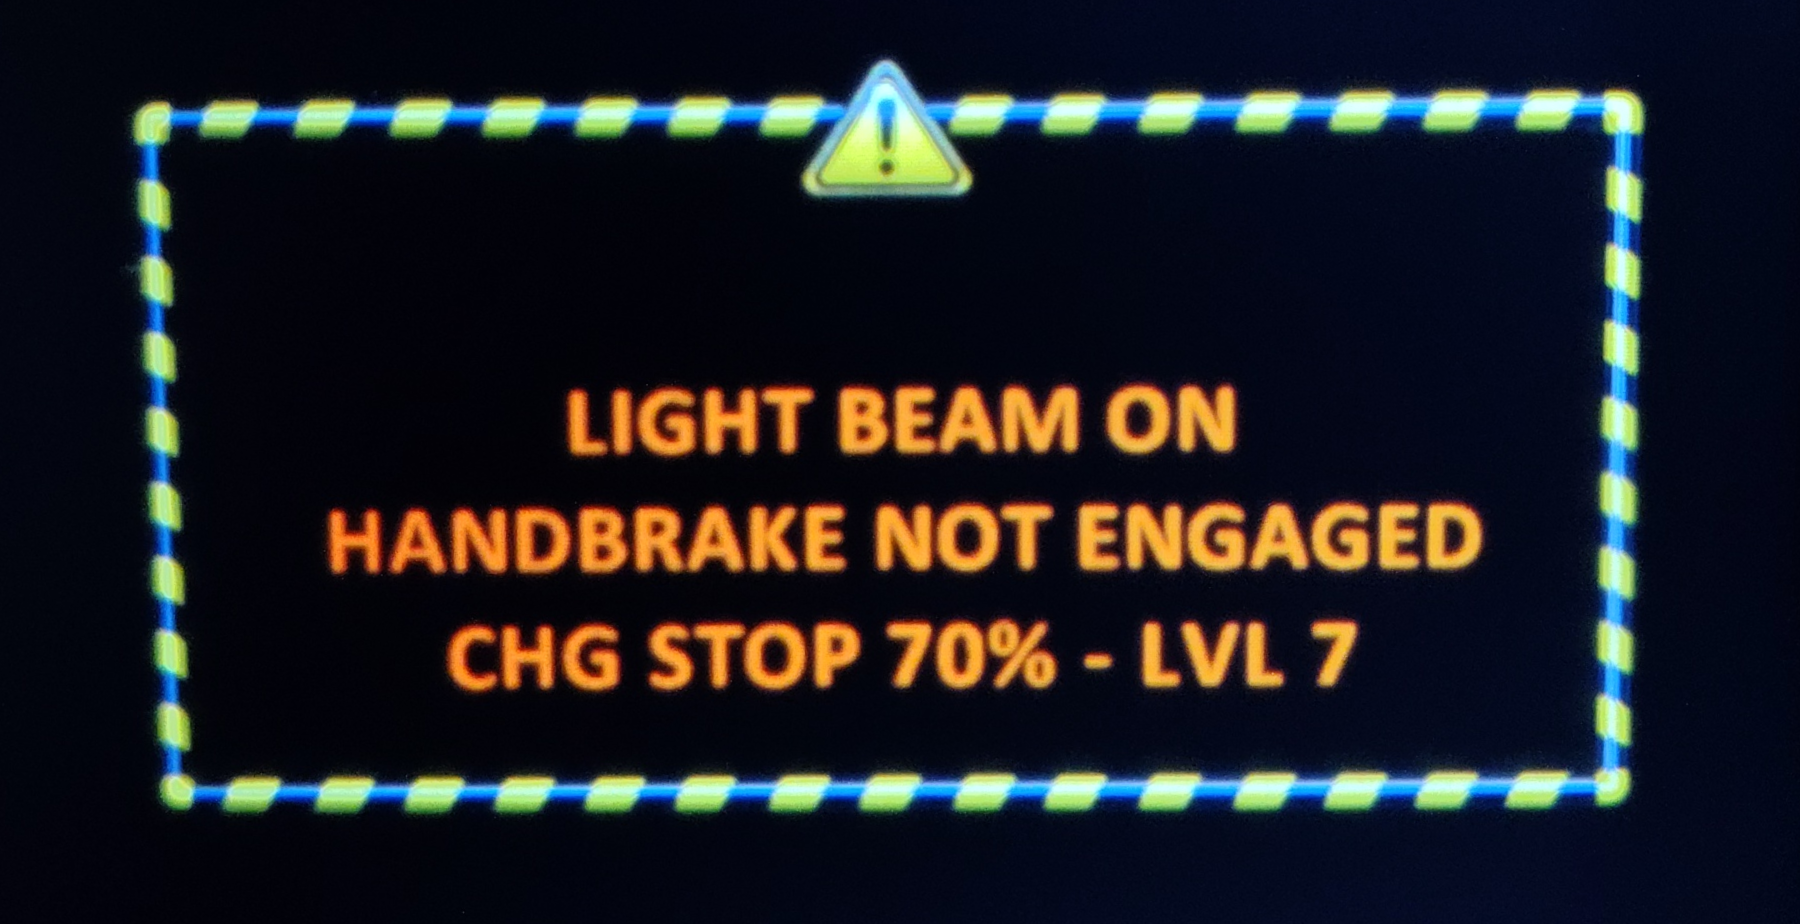
\includegraphics[width=0.5\textwidth]{figures/pop-up_finale.png}
    \caption{Message d'avertissement à l'extinction.}
\end{figure}

Puis, il y a le champ \textbf{« Secondary font colour »} avec un sélecteur de couleur, utilisé pour changer la couleur de la police secondaire sur l'écran du ToM+.

Une autre case disponible est \textbf{« Invert current value sign »}. Si elle est cochée, elle affiche un entier signé pour les valeurs de consommation de courant au lieu de leurs valeurs absolues.\\

Le petit sous-groupe ci-dessous est dédié à la compatibilité du \textbf{Cheatzy} avec ToM+.
Vous pouvez régler votre facteur de triche \textbf{« Cheating factor »} multiplié par 10 : par exemple, 2.0 devient 20.
Vous pouvez également sélectionner si le Cheatzy est activé pendant la charge ou lors du freinage régénératif à l'aide de la case \textbf{« Cheat also Charge/Reku »}. Ces réglages n'ont de sens que si le Cheatzy est connecté et allumé, sinon ils risquent d'altérer vos valeurs de courant de manière incorrecte.\\

Ensuite, se trouve une autre option : \textbf{« Increase thermal protection threshold »}, utilisée pour augmenter de 15°C le seuil de sécurité de surchauffe pour ToM+ durant les saisons les plus chaudes.

Les deux valeurs suivantes sont des configurations supplémentaires pour le calcul du kilométrage restant \textbf{Remaining KM} de ToM+, basé sur l'échantillonnage de la consommation récente. Ici, vous pouvez ajuster la fréquence de l'échantillonnage (par défaut : un par minute) dans \textbf{« Remaining KM sampling time (min) »} et la part du dernier échantillon dans le calcul total (par défaut : 10 \%) dans \textbf{« Remaining KM sample weight (\%) »}.\\

Enfin, nous avons la case \textbf{« Miles to Kilometers »}, qui aide lorsque votre BigToM est issu d'un tableau de bord en miles mais que vous souhaitez le km/h comme unité de mesure. Si elle est activée, ToM+ effectuera cette conversion pour vous.

Pensez à \textbf{enregistrer vos modifications} en appuyant sur le bouton \textbf{« SAVE »} au bas de ce tableau. Si vous ne le faites pas, vos modifications seront perdues lorsque vous quitterez la page.

\begin{figure}[H]
    \centering
    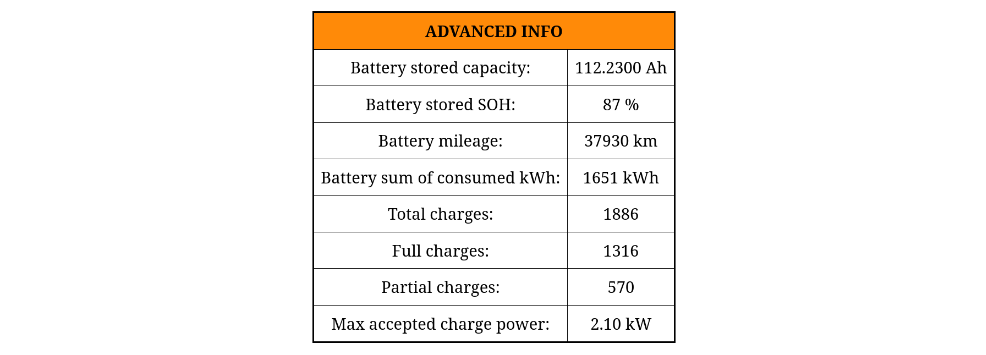
\includegraphics[width=0.9\textwidth]{figures/adv_info.png}
    \caption{Page des infos avancées --- Tableau des infos avancées.}
\end{figure}

Le tableau ci-dessus contient des données relatives à votre batterie, telles que la capacité stockée, la santé \textbf{SOH}, le \textbf{kilométrage de la batterie}, le total de kWh consommés, ainsi que sur les charges, comme le nombre de charges \textit{totales}, \textit{complètes} et \textit{partielles}, et la \textbf{puissance de charge maximale acceptée}.\\

\begin{figure}[H]
    \centering
    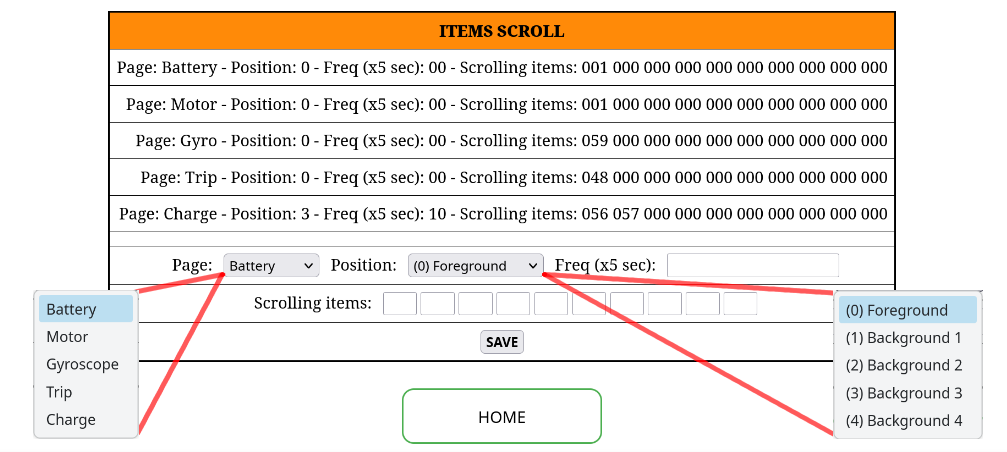
\includegraphics[width=1\textwidth]{figures/item_scroll.png}
    \caption{Page des infos avancées --- Tableau du défilement des éléments.}
\end{figure}

Ce dernier tableau est une fonctionnalité très particulière introduite il y a quelques mises à jour, qui vous permet d'avoir des éléments qui changent dynamiquement dans les pages de votre choix. Cela peut s'appliquer aux pages \textit{batterie}, \textit{moteur}, \textit{gyroscope}, \textit{trajet} et \textit{charge}, et vous pouvez choisir laquelle grâce au champ \textbf{« Page »}.

Ensuite, vous pouvez sélectionner l'emplacement où vous souhaitez faire défiler les éléments de données de votre choix. Pour cela, utilisez le champ \textbf{« Position »} et choisissez dans la liste celui que vous préférez, en vous référant à la Figure~\ref{fig:icon_arrangement} pour la disposition des éléments.\\

Le champ \textbf{« Freq »} correspond à la fréquence de défilement, c'est-à-dire le temps pendant lequel chaque donnée reste affichée à cet emplacement avant de passer à la suivante. Comme vous pouvez le remarquer, il est spécifié entre parenthèses que le champ sera multiplié par \textit{5 secondes}. Cela signifie que la saisie de la valeur \textit{1} entraînera une fréquence de \textit{5 secondes}, la valeur \textit{2} entraînera une fréquence de \textit{10 secondes}, et ainsi de suite.

La partie la plus importante consiste à choisir les éléments à faire défiler : vous pouvez sélectionner jusqu'à dix valeurs de données. Dans les zones de texte \textbf{« Scrolling items »}, insérez la liste des numéros d'éléments souhaités (par ex. 59 ou 48), un par zone, en vous référant aux numéros entre parenthèses dans la liste de la Section~\ref{sec:item_numbers}.\\

Pensez toujours à enregistrer vos modifications en appuyant sur le bouton \textbf{« SAVE »} en bas de ce tableau. Si vous ne le faites pas, vos modifications seront perdues quand vous quitterez la page.

Si vous souhaitez \textbf{désactiver} la fonction de défilement pour une page et une position spécifiques, sélectionnez ces champs puis saisissez \textit{0} dans la zone de texte \textbf{« Freq »}. Juste après, appuyez sur \textbf{« SAVE »} et le défilement se désactivera, revenant aux valeurs par défaut.

Appuyez sur le bouton vert \textbf{« HOME »} en bas du tableau pour revenir à la page d'accueil.



\subsection{Préférences de charge \& Journal}
\label{sec:web_charging_prefs}

Cette page se divise en deux tableaux principaux : le premier sert à contrôler le processus de charge, tandis que le second contient la liste des 15 dernières charges accompagnées de données supplémentaires.

\subsubsection{Préférences de charge}

En commençant par les plus utiles, nous avons le champ \textbf{« Charging status »} qui contient les informations sur le statut actuel de la voiture, y compris le \textit{secteur 220V} et le \textit{processus de charge} avec leurs drapeaux ON et OFF.

Juste en dessous se trouve la case \textbf{« Charge power limit »}, où vous pouvez choisir la puissance que votre Twizy peut utiliser pendant la charge, allant de $0,4 kW$ jusqu'à $2,3 kW$ avec 7 niveaux au choix (sélectionnez \textit{0 pour désactiver la limite de puissance}).

Dans le coin supérieur droit se trouve le bouton \textbf{« ABORT CHARGING »}, qui interrompt immédiatement et proprement le processus de charge, tout comme celui présent sur l'écran du ToM+ dans la page de réglages que nous avons abordée dans la Section~\ref{sec:settings_page}.

\begin{figure}[H]
    \centering
    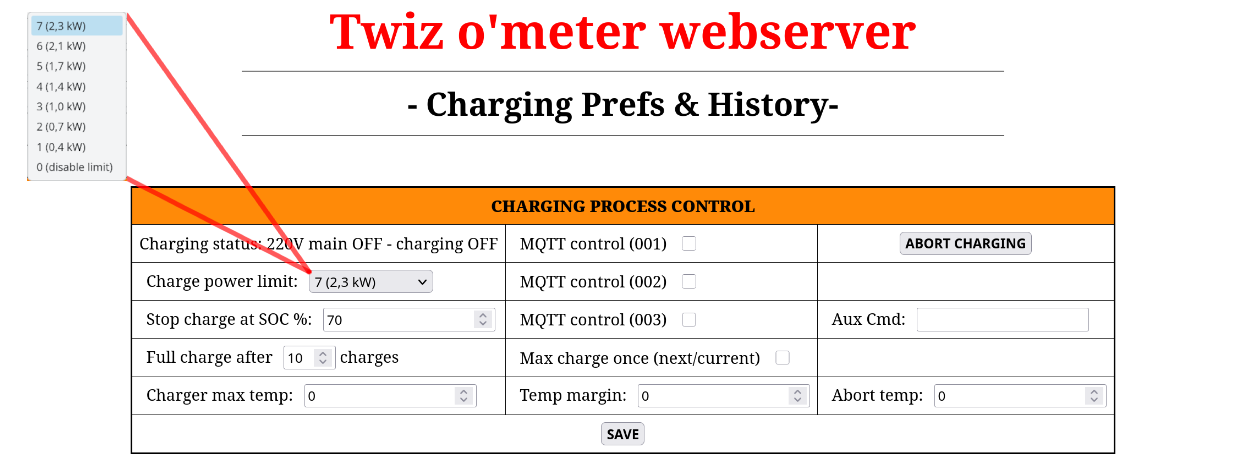
\includegraphics[width=1\textwidth]{figures/charging_process.png}
    \caption{Page des préférences de charge --- Tableau de contrôle du processus de charge.}
\end{figure}

Juste après se trouve le champ \textbf{« Stop charge at SOC \% »}, qui correspond au pourcentage de charge auquel ToM+ envoie automatiquement le signal d'interruption du processus de charge.
Pour votre information, limiter la plage de charge maximale (95 \% ou moins) ralentira la dégradation du SOH de la batterie.

En passant au champ suivant, nous avons le champ \textbf{« Full charge after »} qui est étroitement lié au précédent. En clair, cela n'arrêtera pas la charge au SOC sélectionné une fois toutes les \textit{X} charges (\textit{par exemple 10} comme sur l'image).
Gardez à l'esprit qu'une charge à 100 \% de temps en temps est utile pour rééquilibrer la tension des cellules de la batterie.

Un autre champ associé est l'option \textbf{« Max charge once (next/current) »}, qui fonctionne comme un bouton et ordonne à ToM+ d'effectuer une charge complète sans l'interruption au SOC choisi. Cela prévaut sur le champ précédent et s'appliquera, \textbf{après avoir appuyé sur « SAVE »}, au processus de charge en cours s'il a déjà commencé ou au suivant dans le cas contraire.\\


Nous avons ensuite un champ de sécurité, \textbf{« Charger max temperature »}, dans lequel vous pouvez définir un seuil (valeur entière exprimée en °C). Si ce seuil est dépassé avec une marge d'hystérésis définie par l'utilisateur, ToM+ réduit progressivement le niveau de limite de puissance que nous avons vu auparavant. Il continue de la réduire, de deux niveaux si nécessaire, jusqu'à ce que la température redevienne normale, entraînant le retour à la normale de la limite de puissance.

La marge susmentionnée est personnalisable dans le champ approprié \textbf{« Temp margin »}, où vous pouvez saisir une valeur entière (exprimée en °C), qui sera ajoutée à la température maximale du chargeur pour assouplir le seuil avant de réduire la puissance de charge.

Un autre champ associé est \textbf{« Abort temperature »}, qui contient le dernier seuil de sécurité pour la température du chargeur. S'il est dépassé, ToM+ interrompt immédiatement la charge.\\


Ensuite, nous avons trois champs de contrôle MQTT, distingués par leur numéro progressif.
Cocher l'un de ces drapeaux vous permet de configurer à distance le paramètre situé à sa gauche via le protocole MQTT. Pour ce faire, après avoir activé le champ approprié et \textbf{appuyé sur « SAVE »}, il vous suffira de publier un message MQTT sur le topic spécifié entre parenthèses (ex. \textit{001} ou \textit{002}) sur votre broker (configuré dans la Section~\ref{sec:mqtt_connection}).

Si vous activez le \textbf{MQTT control (001)}, vous pouvez démarrer et arrêter la charge en publiant soit \textit{0} soit \textit{1} sur le topic MQTT \textit{001}.
Il en va de même pour le \textbf{MQTT control (002)} en publiant sur \textit{002} une valeur comprise entre \textit{0} et \textit{7}, et le \textbf{MQTT control (003)} sur \textit{003} avec une valeur comprise entre \textit{0} et \textit{100}.\\

Enfin, nous trouvons le champ \textbf{« Aux Cmd »}, qui désigne la commande auxiliaire et se comporte comme celui que nous avons déjà abordé dans la page des déclencheurs d'alarme de la Section~\ref{sec:web_alarm_triggers}. Il est envoyé lorsque la charge est terminée ou lorsque la charge s'arrête au SOC spécifié.\\


Après toute modification, appuyez sur le bouton \textbf{« SAVE »} pour \textit{enregistrer vos changements}, sinon ils seront perdus lorsque vous quitterez la page.

\subsubsection{Historique de charge}

Le tableau de l'historique de charge conserve les quinze derniers processus de charge ainsi que des valeurs utiles pour les enrichir. Comme vous pouvez le constater, on y retrouve la date et l'heure, ainsi que la valeur des \textbf{kilomètres ODO} au début de la charge. À côté, nous avons la durée de la charge et la puissance moyenne \textbf{Average Power}, ainsi que les kWh rechargés \textbf{charged kWh}.
Enfin, nous avons le \textit{init SOC} et le \textit{end SOC}, qui correspondent aux pourcentages de début et de fin de charge.\\


La dernière colonne contient des \textbf{Notes} supplémentaires sur l'état de la charge, comme la façon dont elle s'est arrêtée (soit le SOC d'arrêt a été atteint, soit l'arrêt a été manuel) ou si elle est toujours en cours.

Si vous le souhaitez, vous pouvez également supprimer manuellement certains enregistrements en appuyant sur le bouton \textit{X} à la fin de l'enregistrement concerné. Il est possible de tous les supprimer d'un coup en appuyant sur le bouton \textbf{« CLEAR HISTORY »} situé dans la partie inférieure du tableau.


\begin{figure}[H]
    \centering
    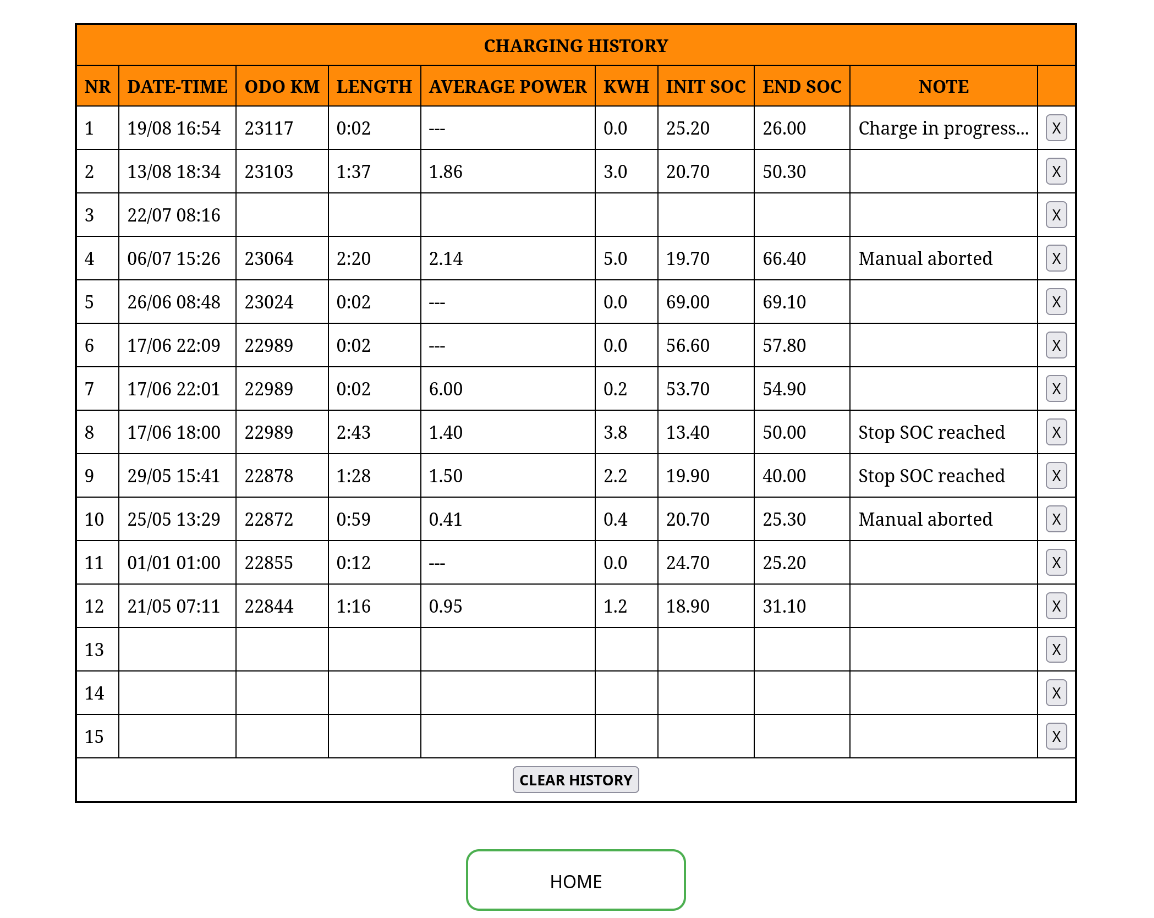
\includegraphics[width=0.95\textwidth]{figures/charging_history.png}
    \caption{Page des préférences de charge --- Tableau de l'historique de charge.}
\end{figure}

Appuyez sur le bouton vert \textbf{« HOME »} sous le dernier tableau pour revenir à la page d'accueil.

\clearpage

\subsection{Page Heure \& Date}
\label{sec:web_time_date}

Avec votre ToM+, vous pouvez consulter la date et l'heure actuelles, mais comment les régler ?
Cette page a été conçue exactement à cet effet et ne contient qu'un seul tableau présenté sur l'image ci-dessous.

\begin{figure}[H]
    \centering
    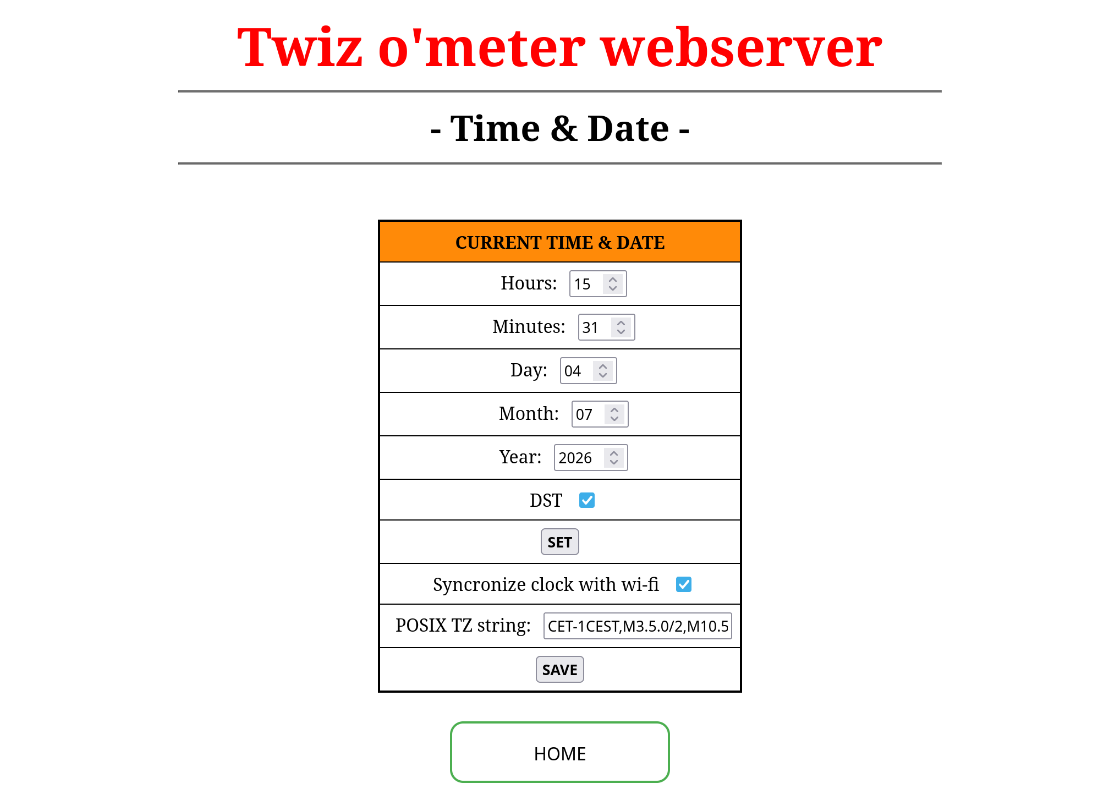
\includegraphics[width=1\textwidth]{figures/time_page.png}
    \caption{Tableau de l'Heure \& Date actuelles.}
\end{figure}

Les cinq premiers champs sont explicites et intuitifs, il suffit de régler la date et l'heure en fonction de votre fuseau horaire. La case à cocher \textbf{« DST »}, qui signifie Daylight Saving Time (Heure d'été), vous permet d'activer ou de désactiver le décalage d'une heure selon la saison.

Lorsque vous souhaitez confirmer vos modifications et les appliquer à ToM+, appuyez simplement sur le bouton \textbf{« SET »} et elles seront mises à jour.\\

Ensuite, nous avons un champ très utile, l'option \textbf{« Synchronize clock with WiFi »}, pratique lorsque vous avez déjà configuré une connexion Wi-Fi comme expliqué dans la Section~\ref{sec:add_wifi_profile}. Activez-la simplement et laissez ToM+ faire le travail.

Juste en dessous se trouve une valeur plus technique concernant la date et l'heure qui indique à ToM+ quel est votre fuseau horaire actuel (\textbf{TZ}) à l'aide d'une chaîne appelée \textbf{« POSIX »}. Cela inclut le moment où le décalage d'une heure de l'heure d'été est appliqué. Dans la plupart des pays d'Europe centrale, la chaîne est la suivante : \textit{CET-1CEST,M3.5.0/2,M10.5.0/3}. Recherchez sur Internet la chaîne POSIX TZ de votre pays en cas de doute.\\


Comme toujours, n'oubliez pas d'enregistrer vos modifications en appuyant sur le bouton \textbf{« SAVE »} au bas du tableau, sinon elles seront perdues quand vous quitterez la page.

Appuyez sur le bouton vert \textbf{« HOME »} sous le tableau pour revenir à la page d'accueil.

\clearpage

\subsection{Page des réglages BigToM / ToM+}
\label{sec:web_btom_tom_sets}

Sur cette page, vous pouvez personnaliser certains paramètres de votre BigToM ou ToM+, car cette page contient principalement des configurations pour la \textbf{page du tableau de bord}, disponible uniquement sur ces deux appareils.

\begin{figure}[H]
    \centering
    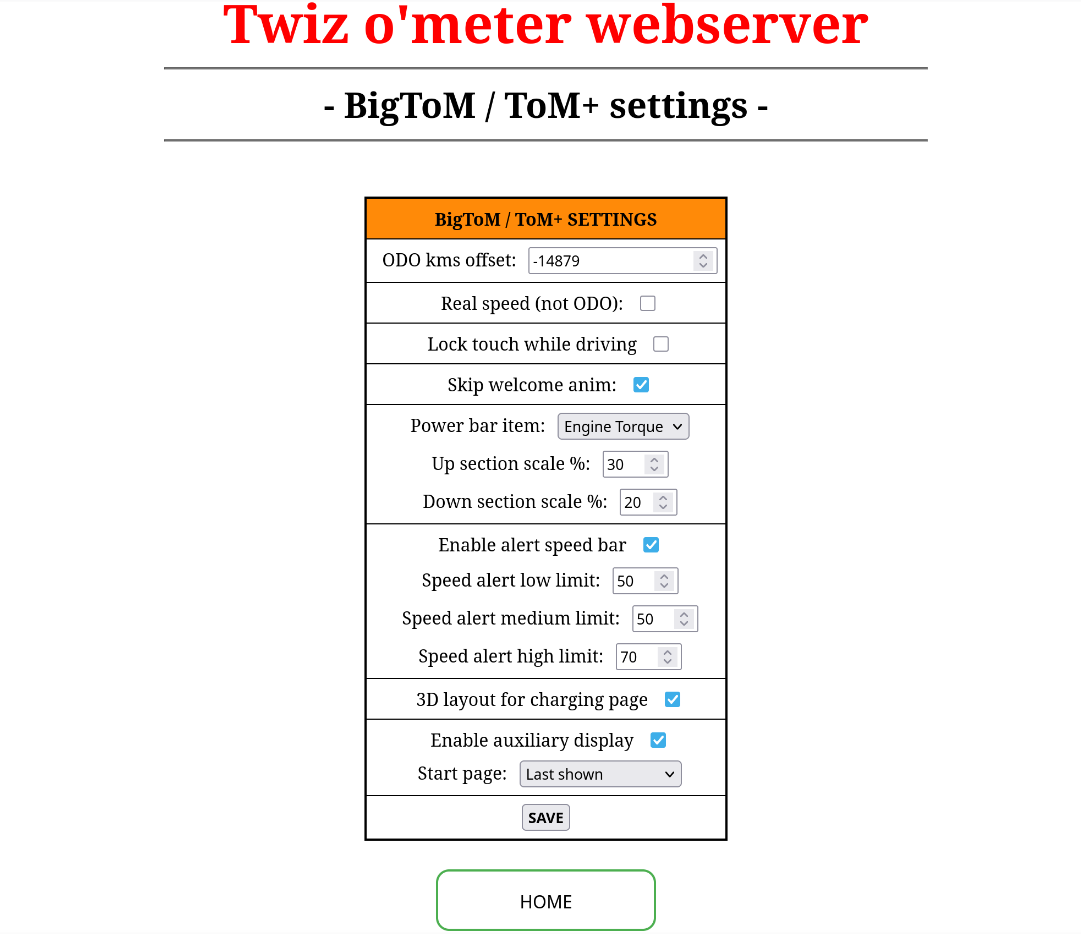
\includegraphics[width=1\textwidth]{figures/btom_page.png}
    \caption{Tableau des réglages BigToM \textbackslash ToM+.}
\end{figure}

Lors du remplacement de votre tableau de bord par un BigToM, vous devrez peut-être ajouter ou soustraire des kilomètres à l'ODO du nouveau tableau de bord pour retrouver votre kilométrage d'origine. En effet, ils sont stockés dans la carte mère du tableau de bord. Ainsi, le premier paramètre est le champ \textbf{« ODO kms offset »}, utilisé pour corriger cette différence de kilomètres.

Comme vous le savez peut-être, les indicateurs de vitesse du tableau de bord sont délibérément majorés de $3 km/h$ pour des raisons de sécurité. Si vous souhaitez voir votre vitesse réelle, activez simplement l'option \textbf{« Real speed (not ODO) »} dans la deuxième ligne du tableau.\\

Examinons maintenant l'option \textbf{« Lock touch while driving »}. Si elle est active, l'écran tactile sera désactivé pendant la conduite (c'est-à-dire vitesse $>0$) pour des raisons de sécurité.

Ensuite, nous avons l'option \textbf{Skip welcome animation}, qui peut être activée si vous êtes lassé de voir l'animation de bienvenue lors du passage du tableau de bord à une autre page.\\


Il y a ensuite une section dédiée à la barre de puissance montrée sur la Figure~\ref{fig:dashboard_layout} en haut de la disposition du tableau de bord. Vous pouvez choisir ici, en utilisant la zone de choix \textbf{« Power bar item »}, quelle valeur doit être affichée et utilisée pour remplir la barre de puissance. Il y a trois données disponibles : \textit{Engine Torque} (Couple moteur), \textit{Battery Ampere} (Ampérage batterie) ou \textit{Battery kW} (Kilowatts batterie).

Les deux champs \textbf{« Up/Down section scale \% »} ci-dessous servent à ajuster la plage de la barre de puissance et représentent le pourcentage de la valeur maximale/minimale de l'élément de donnée sélectionné.
Dans l'image d'exemple, pour la plage maximale, j'ai indiqué \textit{30\%}.\\


Dans la section suivante, nous pouvons activer une autre fonctionnalité intéressante, présentée également sur la Figure~\ref{fig:dashboard_layout}, juste en dessous de l'indicateur de vitesse. Cela s'effectue en activant la case \textbf{« Enable alert speed bar »}, qui comporte trois seuils personnalisables, chacun correspondant à une couleur allant du \textit{vert} au \textit{jaune} puis au \textit{rouge}.

Les trois champs suivants, \textbf{« Speed alert low/medium/high limit »}, sont destinés à être remplis avec les vitesses de seuil respectives en $km/h$ pour allumer la barre de vitesse avec la couleur appropriée. Dans l'exemple, la barre deviendra jaune en dépassant $50 km/h$ puis rouge en dépassant $70 km/h$. Comme vous pouvez le remarquer, je ne voulais pas que la barre verte s'affiche, j'ai donc réglé la valeur du seuil \textit{low} sur la même valeur que le seuil \textit{medium}.\\


L'avant-dernière fonction est l'option \textbf{« 3D layout for charging page »}, activée par défaut, qui affiche des détails en 3D au lieu de la page de charge ToM standard.

Et enfin, la fonctionnalité la plus récemment ajoutée s'appelle le \textbf{Twin ToM}, conçue pour les propriétaires du ToM d'origine avant la sortie du ToM+. Cela vous permet d'utiliser le plus petit écran en combinaison avec la nouvelle version à clipser, afin de surveiller deux pages simultanément. Mais pour que cela fonctionne, vous devez activer l'option de la dernière ligne, \textbf{« Enable auxiliary display »}.

Vous pouvez ensuite sélectionner, avec la zone de choix \textbf{« Start page »}, une page spécifique à afficher sur l'écran auxiliaire lors de l'allumage, ou simplement choisir \textit{Last shown} (Dernière affichée).\\


Comme toujours, n'oubliez pas d'enregistrer vos modifications en appuyant sur le bouton \textbf{« SAVE »} en bas du tableau, sinon elles seront perdues lorsque vous quitterez la page.

Appuyez sur le bouton vert \textbf{« HOME »} sous le tableau pour revenir à la page d'accueil.

\clearpage

\subsection{Page de diagnostic}
\label{sec:web_diagnostic}

Cette page se compose d'un seul tableau et vous permet de consulter plus d'informations sur les 10 dernières erreurs survenues sur votre Twizy, de manière similaire à la page d'affichage du ToM+ abordée dans la Section~\ref{sec:error_page}.

Les valeurs affichées sont le \textbf{« DTC Number »} et, si disponible, le \textbf{« DF Number »}, qui sont des identifiants uniques pour les erreurs de la Twizy, vous permettant de faire des recherches en ligne.
Ensuite, nous avons le statut de l'erreur \textbf{« Status »}, tel que \textit{SAVED} si elle s'est déjà produite ou \textit{PRESENT} si elle vient tout juste de se produire.

Pour \textit{activer les numéros DF}, veuillez vous référer à la Section~\ref{sec:add_wifi_profile}.

\begin{figure}[H]
    \centering
    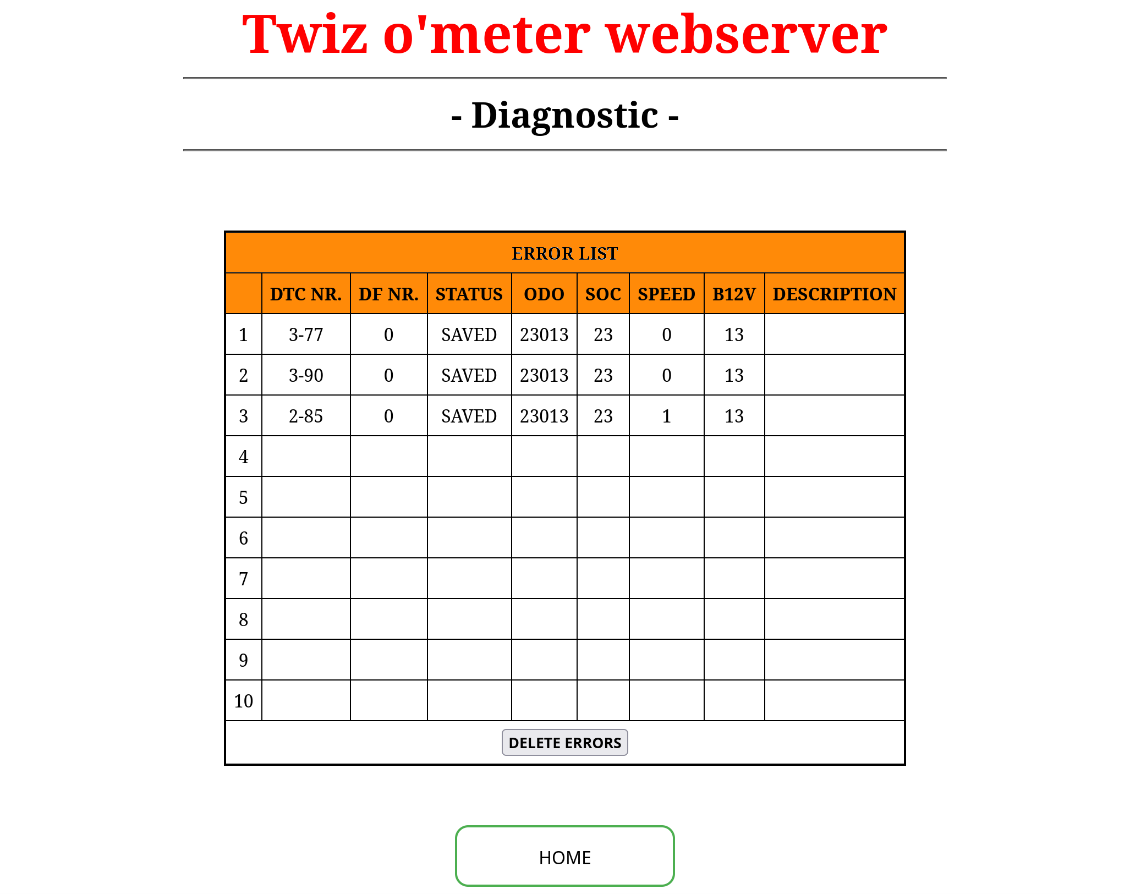
\includegraphics[width=1\textwidth]{figures/error_page.png}
    \caption{Page de diagnostic --- Tableau de la liste des erreurs.}
\end{figure}

En plus de ces valeurs, les quatre valeurs suivantes sont les références d' \textbf{« ODO »}, de \textbf{« SOC »}, de \textbf{« speed »} et de \textbf{« 12V Battery voltage »} au moment où l'erreur correspondante s'est produite.

Pour chaque enregistrement d'erreur, s'il est disponible, il existe un champ de description d'erreur \textbf{« Description »}.\\


Si vous souhaitez effacer les erreurs de la Twizy, y compris les erreurs fatales, vous pouvez appuyer sur le bouton \textbf{« DELETE ERRORS »} ci-dessous, qui les supprimera toutes en une seule fois.

Appuyez sur le bouton vert \textbf{« HOME »} situé sous le tableau pour revenir à la page d'accueil.